% Options for packages loaded elsewhere
\PassOptionsToPackage{unicode}{hyperref}
\PassOptionsToPackage{hyphens}{url}
%
\documentclass[
]{book}
\usepackage{amsmath,amssymb}
\usepackage{lmodern}
\usepackage{iftex}
\ifPDFTeX
  \usepackage[T1]{fontenc}
  \usepackage[utf8]{inputenc}
  \usepackage{textcomp} % provide euro and other symbols
\else % if luatex or xetex
  \usepackage{unicode-math}
  \defaultfontfeatures{Scale=MatchLowercase}
  \defaultfontfeatures[\rmfamily]{Ligatures=TeX,Scale=1}
\fi
% Use upquote if available, for straight quotes in verbatim environments
\IfFileExists{upquote.sty}{\usepackage{upquote}}{}
\IfFileExists{microtype.sty}{% use microtype if available
  \usepackage[]{microtype}
  \UseMicrotypeSet[protrusion]{basicmath} % disable protrusion for tt fonts
}{}
\makeatletter
\@ifundefined{KOMAClassName}{% if non-KOMA class
  \IfFileExists{parskip.sty}{%
    \usepackage{parskip}
  }{% else
    \setlength{\parindent}{0pt}
    \setlength{\parskip}{6pt plus 2pt minus 1pt}}
}{% if KOMA class
  \KOMAoptions{parskip=half}}
\makeatother
\usepackage{xcolor}
\IfFileExists{xurl.sty}{\usepackage{xurl}}{} % add URL line breaks if available
\IfFileExists{bookmark.sty}{\usepackage{bookmark}}{\usepackage{hyperref}}
\hypersetup{
  pdftitle={Statistical Modeling for the Biological Sciences},
  pdfauthor={Eric M Reyes},
  hidelinks,
  pdfcreator={LaTeX via pandoc}}
\urlstyle{same} % disable monospaced font for URLs
\usepackage{longtable,booktabs,array}
\usepackage{calc} % for calculating minipage widths
% Correct order of tables after \paragraph or \subparagraph
\usepackage{etoolbox}
\makeatletter
\patchcmd\longtable{\par}{\if@noskipsec\mbox{}\fi\par}{}{}
\makeatother
% Allow footnotes in longtable head/foot
\IfFileExists{footnotehyper.sty}{\usepackage{footnotehyper}}{\usepackage{footnote}}
\makesavenoteenv{longtable}
\usepackage{graphicx}
\makeatletter
\def\maxwidth{\ifdim\Gin@nat@width>\linewidth\linewidth\else\Gin@nat@width\fi}
\def\maxheight{\ifdim\Gin@nat@height>\textheight\textheight\else\Gin@nat@height\fi}
\makeatother
% Scale images if necessary, so that they will not overflow the page
% margins by default, and it is still possible to overwrite the defaults
% using explicit options in \includegraphics[width, height, ...]{}
\setkeys{Gin}{width=\maxwidth,height=\maxheight,keepaspectratio}
% Set default figure placement to htbp
\makeatletter
\def\fps@figure{htbp}
\makeatother
\setlength{\emergencystretch}{3em} % prevent overfull lines
\providecommand{\tightlist}{%
  \setlength{\itemsep}{0pt}\setlength{\parskip}{0pt}}
\setcounter{secnumdepth}{5}
\newlength{\cslhangindent}
\setlength{\cslhangindent}{1.5em}
\newlength{\csllabelwidth}
\setlength{\csllabelwidth}{3em}
\newlength{\cslentryspacingunit} % times entry-spacing
\setlength{\cslentryspacingunit}{\parskip}
\newenvironment{CSLReferences}[2] % #1 hanging-ident, #2 entry spacing
 {% don't indent paragraphs
  \setlength{\parindent}{0pt}
  % turn on hanging indent if param 1 is 1
  \ifodd #1
  \let\oldpar\par
  \def\par{\hangindent=\cslhangindent\oldpar}
  \fi
  % set entry spacing
  \setlength{\parskip}{#2\cslentryspacingunit}
 }%
 {}
\usepackage{calc}
\newcommand{\CSLBlock}[1]{#1\hfill\break}
\newcommand{\CSLLeftMargin}[1]{\parbox[t]{\csllabelwidth}{#1}}
\newcommand{\CSLRightInline}[1]{\parbox[t]{\linewidth - \csllabelwidth}{#1}\break}
\newcommand{\CSLIndent}[1]{\hspace{\cslhangindent}#1}
%%%%%%%%%%%%%%%%%%%%%%%%%%%%%%%%%%%%%%%%%%%%%%%%%%%%%%%%%%%%%%%%%%%%%%%%%%%%%%%%
% File: style.tex
% Description: Create look for PDF version of text.




%%%%%%%%%%%%%%%%%%%%%%%%%%%%%%%%%%%%%%%%%%%%%%%%%%%%%%%%%%%%%%%%%%%%%%%%%%%%%%%%
% Theorem Environments
\usepackage{amsthm}

\makeatletter
\newtheoremstyle{mydefn}% name of the style to be used
{\baselineskip}% measure of space to leave above the theorem. E.g.: 3pt
{\baselineskip}% measure of space to leave below the theorem. E.g.: 3pt
{\addtolength{\@totalleftmargin}{1em}%
  \addtolength{\linewidth}{-1em}%
  \parshape 1 1em \linewidth
  \slshape}% name of font to use in the body of the theorem
{}% measure of space to indent
{\bfseries}% name of head font
{:}% punctuation between head and body
{\newline}% space after theorem head; " " = normal interword space
{}% Manually specify head
\makeatother

\makeatletter
\newtheoremstyle{myexmpl}% name of the style to be used
{\baselineskip}% measure of space to leave above the theorem. E.g.: 3pt
{\baselineskip}% measure of space to leave below the theorem. E.g.: 3pt
{\addtolength{\@totalleftmargin}{1em}%
  \addtolength{\linewidth}{-1em}%
  \parshape 1 1em \linewidth}% name of font to use in the body of the theorem
{}% measure of space to indent
{\bfseries}% name of head font
{}% punctuation between head and body
{\newline}% space after theorem head; " " = normal interword space
{\thmname{#1}\thmnumber{ #2}:\thmnote{ {\mdseries``#3''}}}% Manually specify head
\makeatother


\theoremstyle{plain}
\newtheorem{theorem}{Theorem}[chapter]
\newtheorem{lemma}{Lemma}[chapter]

\theoremstyle{mydefn}
\newtheorem{definition}{Definition}[chapter]
\newtheorem{corollary}{Corollary}[chapter]
\newtheorem{proposition}{Proposition}[chapter]

\theoremstyle{myexmpl}
\newtheorem{example}{Example}[chapter]
\newtheorem{exercise}{Exercise}[chapter]

\theoremstyle{remark}
\newtheorem*{remark}{Remark}
\newtheorem*{solution}{Solution}


%%%%%%%%%%%%%%%%%%%%%%%%%%%%%%%%%%%%%%%%%%%%%%%%%%%%%%%%%%%%%%%%%%%%%%%%%%%%%%%%
% New Environments for Custom Blocks

\graphicspath{{./images/}}
\usepackage{tikz}
\usepackage{tcolorbox}
\tcbuselibrary{skins}

\definecolor{rhitred}{HTML}{800000}


\newcommand{\mytitle}[1]{
  \node[fill=rhitred,
  rounded corners,
  draw=white,
  line width=2pt,
  text width=4cm,
  inner sep=8pt,
  xshift=-2cm]
  at (frame.north){\bfseries\textcolor{white}{#1}};
}

\newtcolorbox{rmdfivefund}{
  enhanced,
  overlay={\mytitle{Fundamental Idea:}},
  borderline={2pt}{0mm}{rhitred},
  borderline={.7pt}{1mm}{rhitred},
  frame hidden,
  sidebyside,
  sidebyside align = top seam,
  lefthand width = 2em,
  arc=3mm,
  segmentation hidden,
  top=15pt,
  before upper={
\includegraphics[scale=0.05]{Icon_FundamentalIdea.png}\tcblower}
}

\newtcolorbox{rmdkeyidea}{
  enhanced,
  borderline={2pt}{0mm}{rhitred},
  borderline={.7pt}{1mm}{rhitred},
  frame hidden,
  sidebyside,
  sidebyside align = top seam,
  lefthand width = 2em,
  arc=3mm,
  segmentation hidden,
  top=15pt,
  before upper={
\includegraphics[scale=0.05]{Icon_KeyIdea.png}\tcblower}
}

\newtcolorbox{rmdwarning}{
  enhanced,
  borderline={2pt}{0mm}{rhitred},
  borderline={.7pt}{1mm}{rhitred},
  frame hidden,
  sidebyside,
  sidebyside align = top seam,
  lefthand width = 2em,
  arc=3mm,
  segmentation hidden,
  top=15pt,
  before upper={
\includegraphics[scale=0.04]{Icon_Tip.png}\tcblower}
}

\newtcolorbox{rmdtip}{
  enhanced,
  borderline={2pt}{0mm}{rhitred},
  borderline={.7pt}{1mm}{rhitred},
  frame hidden,
  sidebyside,
  sidebyside align = top seam,
  lefthand width = 2em,
  arc=3mm,
  segmentation hidden,
  top=15pt,
  before upper={
\includegraphics[scale=0.035]{Icon_Warning.png}\tcblower}
}

\let\BeginKnitrBlock\begin \let\EndKnitrBlock\end

%\newenvironment{rmdkeyidea}%
%  {\begin{center}
%    \begin{tabular}{|p{0.9\textwidth}|}
%    \hline\\
%    \textbf{Key Idea: }
%  }
%  {
%  \\\\\hline
%  \end{tabular}
%  \end{center}
%  }
%
%\newenvironment{rmdfivefund}%
%  {\begin{center}
%    \begin{tabular}{|p{0.9\textwidth}|}
%    \hline\\
%    \textbf{Fundamental Idea: }
%  }
%  {
%  \\\\\hline
%  \end{tabular}
%  \end{center}
%  }
%
%\newenvironment{rmdwarning}%
%  {\begin{center}
%    \begin{tabular}{|p{0.9\textwidth}|}
%    \hline\\
%    \textbf{Warning: }
%  }
%  {
%  \\\\\hline
%  \end{tabular}
%  \end{center}
%  }
%
%\newenvironment{rmdtip}%
%  {\begin{center}
%    \begin{tabular}{|p{0.9\textwidth}|}
%    \hline\\
%    \textbf{Tip: }
%  }
%  {
%  \\\\\hline
%  \end{tabular}
%  \end{center}
%  }

\usepackage{booktabs}
\usepackage{longtable}
\usepackage{array}
\usepackage{multirow}
\usepackage{wrapfig}
\usepackage{float}
\usepackage{colortbl}
\usepackage{pdflscape}
\usepackage{tabu}
\usepackage{threeparttable}
\usepackage{threeparttablex}
\usepackage[normalem]{ulem}
\usepackage{makecell}
\usepackage{xcolor}
\ifLuaTeX
  \usepackage{selnolig}  % disable illegal ligatures
\fi

\title{Statistical Modeling for the Biological Sciences}
\author{Eric M Reyes}
\date{Last Updated: 2022-04-07}

\begin{document}
\maketitle

{
\setcounter{tocdepth}{1}
\tableofcontents
}
\newcommand{\norm}[1]{\lVert#1\rVert}
\newcommand{\abs}[1]{\lvert#1\rvert}
\newcommand{\iid}{\stackrel{\text{IID}}{\sim}}
\newcommand{\ind}{\stackrel{\text{Ind}}{\sim}}

\newcommand{\bm}[1]{\mathbf{#1}}
\newcommand{\bs}[1]{\boldsymbol{#1}}
\newcommand{\bbeta}{\bs{\beta}}

\newcommand{\Ell}{\mathcal{L}}

\hypertarget{preface}{%
\chapter*{Preface}\label{preface}}
\addcontentsline{toc}{chapter}{Preface}

The biological sciences often yield datasets which present unique challenges to data analysis. This text introduces these challenges and the statistical methods employed to overcome them. We begin with an introduction to the use of statistical regression models and then explore how such models can be altered to account for various features in the dataset. This could include non-linear or categorical response variables, censored survival (or reliability) data, or repeated measurements on the same subject. Other topics discussed as time permits include pooling results from multiple studies, study design and power, drawing causal conclusions from observational data, missing data, and general modeling techniques.

This text is applied, focusing primarily on knowing when various modeling strategies are appropriate and how to interpret their results. One goal is to enable students to evaluate the strength of evidence presented in the literature within their field of study. As with any text in statistics, we seek to develop your statistical literacy and statistical reasoning. Behind the entire text are the following five fundamental ideas of statistical inference:

\begin{enumerate}
\def\labelenumi{\arabic{enumi}.}
\item
  Research questions can often be framed in terms of a parameter characterizing the variable of interest within the population.
\item
  If data is to be useful for making conclusions about the population, a process referred to as drawing inference, we must consider the method in which the data was collected.
\item
  The use of data for decision making requires the data be summarized and presented in ways that address the question of interest.
\item
  Variability is inherit in any process, and as a result, the data is subject to sampling variability. Statistics vary across samples in a predictable way; that is, they have a distribution which can be modeled.
\item
  With a model for the distribution of a statistic, we can quantify the strength of evidence against a particular hypothesis or construct an estimate of the parameter which accounts for the variability. This allows us to draw conclusions about the corresponding parameter.
\end{enumerate}

\hypertarget{part-review-of-the-inferential-process}{%
\part{Review of the Inferential Process}\label{part-review-of-the-inferential-process}}

\hypertarget{statistical-process}{%
\chapter{The Statistical Process}\label{statistical-process}}

Research is about telling a story, and good data presentation and statistical inference can help tell that story in a compelling way. This chapter cannot replace an introductory course on statistical analysis. Instead, it aims to give practical advice in data storage, preparation, and analysis which are fundamental to our study of statistical models in the biological sciences.

\hypertarget{overview-of-drawing-inference}{%
\section{Overview of Drawing Inference}\label{overview-of-drawing-inference}}

Every research question posed is trying to characterize a \textbf{population}.

\begin{definition}[Population]
The collection of subjects we would like to say something about.
\end{definition}

It is often impossible (or impractical) to observe the entire population. Instead, we make observations on a subset of the population; this smaller group is known as the \textbf{sample}.

\begin{definition}[Sample]
The collection of subjects for which we actually obtain measurements (data).
\end{definition}

For each subject within the sample, we obtain a collection of measurements, which form our data. This could be the result, for example, of a survey, examination of medical records, or a prospective study which follows subjects for a lengthy period of time. The goal of statistical modeling is to use the sample (the group we actually observe) to say something about the population of interest (the group we wish we had observed); this process is known as \textbf{statistical inference} and is illustrated in Figure \ref{fig:statistical-process-statistical-process}.

\begin{definition}[Statistical Inference]
The process of using a sample to characterize some aspect of the underlying population.
\end{definition}

\begin{figure}

{\centering 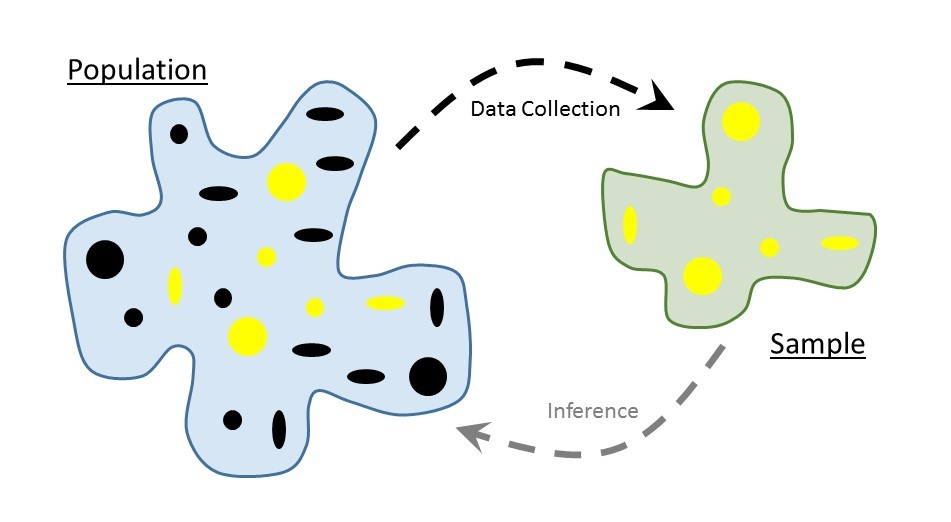
\includegraphics[width=0.8\textwidth]{images/Statistical-Process-Statistical-Process} 

}

\caption{Illustration of the statistical process.}\label{fig:statistical-process-statistical-process}
\end{figure}

\hypertarget{data-storage}{%
\section{Data Storage}\label{data-storage}}

Each measurement, or piece of information, you record for a subject is a different \textbf{variable}.

\begin{definition}[Variable]
A measurement, or category, describing some aspect of the subject.
\end{definition}

In order to conduct analysis, it is best to adhere to tidy data principles (\protect\hyperlink{ref-Wickham2014}{Wickham 2014}) when storing data. In brief:

\begin{enumerate}
\def\labelenumi{\arabic{enumi}.}
\item
  Each column contains a unique variable.
\item
  Each record (or row in the data set) corresponds to a different observation of the variables. If each subject is only measured once (a single survey for each subject, for example), each record will correspond to a different subject. If, on the other hand, each subject is measured multiple times (the same survey is given prior to an appointment and at a specified follow-up period, for example), there may be multiple records which correspond to the same subject, but each record corresponds to a unique observation.
\item
  If you have multiple data sets, there should be a variable in the table that allows the various tables to be linked (subject identifier). For larger more complex studies, for example, you may have one table that has the demographic information of subjects and a separate table which contains the lab results for the subjects.
\item
  The first row in the data set should have the names of each variable.
\end{enumerate}

The above description eliminates a common method of data storage --- placing different groups in different spreadsheets. All observations should be stored together. The first few records of a hypothetical data set are illustrated in Table \ref{tab:statistical-process-tidy-data}.

\begin{table}

\caption{\label{tab:statistical-process-tidy-data}Example of storing data according to "tidy data" principles.  Data is from a hypothetical study.}
\centering
\resizebox{\linewidth}{!}{
\begin{tabular}[t]{rlrrrl}
\toprule
Subject ID & Education & Age (yrs) & Parity & Number of Miscarriages & Treatment Group\\
\midrule
1089 & 0-5yrs & 28 & 6 & 0 & Active Treatment\\
1160 & 0-5yrs & 36 & 1 & 0 & Active Treatment\\
1025 & 0-5yrs & 34 & 6 & 0 & Active Treatment\\
1035 & 0-5yrs & 32 & 4 & 1 & Active Treatment\\
1112 & 6-11yrs & 32 & 3 & 0 & Active Treatment\\
\addlinespace
1030 & 6-11yrs & 33 & 4 & 1 & Active Treatment\\
1159 & 0-5yrs & 26 & 6 & 2 & Placebo\\
1207 & 0-5yrs & 42 & 1 & 0 & Placebo\\
1179 & 0-5yrs & 39 & 6 & 0 & Placebo\\
1014 & 0-5yrs & 34 & 4 & 0 & Placebo\\
\addlinespace
1195 & 6-11yrs & 35 & 3 & 1 & Placebo\\
1170 & 6-11yrs & 36 & 4 & 1 & Placebo\\
\bottomrule
\end{tabular}}
\end{table}

Once your data has been placed in a spreadsheet, it should be kept separate from the analysis. While it may be easy, it is poor practice to include graphics and numeric summaries in the same spreadsheet as the data. If you want your data to be \emph{portable} (easily opened by any spreadsheet or analysis software package), save your data as a comma separated file (CSV).

\hypertarget{tabular-data-presentation}{%
\section{Tabular Data Presentation}\label{tabular-data-presentation}}

If you have several variables you want to summarize, this is probably best done using a table. For example, you may want to summarize the demographics of the subjects in your study across each treatment group. How a variable is summarized depends on its type. \textbf{Qualitative} (or \textbf{categorical}) variables define a grouping or categorization of a subject (e.g., race, treatment group, etc.). When summarizing qualitative data, we generally report the number of subjects in each group and the corresponding percentage of the sample.

\begin{definition}[Categorical Variable]
Also called a ``qualitative variable,'' a measurement on a subject which denotes a grouping or categorization.
\end{definition}

\textbf{Quantitative} (or \textbf{numeric}) variables are those measurements for which arithmetic makes sense (e.g., heart rate, age). These variables are generally summarized by reporting both a measure of location and spread; this could be mean and standard deviation or median and interquartile range.

\begin{definition}[Numeric Variable]
Also called a ``quantitative variable,'' a measurement on a subject which takes on a numeric value \emph{and} for which ordinary arithmetic makes sense.
\end{definition}

If you are not comparing groups of subjects, it is reasonable to report results for the entire sample. If the goal of your research is to compare groups (such as rural vs.~urban residents), we typically summarize data within each group and present the comparisons side by side. Table \ref{tab:statistical-process-data-summary} summarizes the data from our hypothetical study, comparing the treatment and placebo groups.

\begin{table}

\caption{\label{tab:statistical-process-data-summary}Summary of subjects from our hypothetical study. Qualitative variables are summarized as N (pct) and quantitative variables are summarized as mean (standard deviation).}
\centering
\resizebox{\linewidth}{!}{
\begin{tabular}[t]{lcc}
\toprule
Characteristic & Active Treatment & Placebo\\
\midrule
\makecell[l]{Education\\   0-5 years\\   6-11 years\\   12+ years} & \makecell[l]{\\8 (4.8)\\80 (48.5)\\77 (46.7)} & \makecell[l]{\\4 (4.8)\\40 (48.2)\\39 (47)}\\
Age & 30.51 (2.67) & 31.53 (5.28)\\
Parity & 2.08 (1.24) & 2.11 (1.28)\\
Number of Miscarriages & 0.39 (0.62) & 0.95 (0.79)\\
\bottomrule
\end{tabular}}
\end{table}

When reporting numerical summaries within the body of your report, it is good to keep the same format as you adopt in the table; for example, summarizing a qualitative variables with N (\%).

Statistics is generally concerned with explaining the variation in a variable, and that is characterized by its \textbf{distribution}. When we summarize a variable, whether numerically or graphically, we are actually summarizing this distribution.

\begin{definition}[Distribution]
The pattern of variability corresponding to a set of values.
\end{definition}

\hypertarget{graphical-data-presentation}{%
\section{Graphical Data Presentation}\label{graphical-data-presentation}}

As the saying goes, a picture is worth 1000 words. Each graphic you construct, however, should add value to the story you are telling. We primarily reserve graphics for conveying a message about our primary \textbf{response}.

\begin{definition}[Response Variable]
Also called the ``outcome,'' this is the primary variable of interest in the research question; it is the variable we either want to explain or predict.
\end{definition}

As with tabular data presentation, our approach to graphical presentation depends on the type of variable being summarized. For example, while a scatter-plot is well suited for examining the relationship between two quantitative variables, side-by-side box-plots are better suited for examining the relationship between a quantitative response and a categorical predictor. Following best practices in the research community, we recommend the use of a \emph{bar chart} instead of a \emph{pie chart} when examining a categorical response. Bar charts are often less cluttered and more clearly communicate the same information.

Figure \ref{fig:statistical-process-graphics} illustrates two graphics (one for qualitiative and one for quantitative response); again, your graphics should be driven by your research question.

\begin{figure}

{\centering 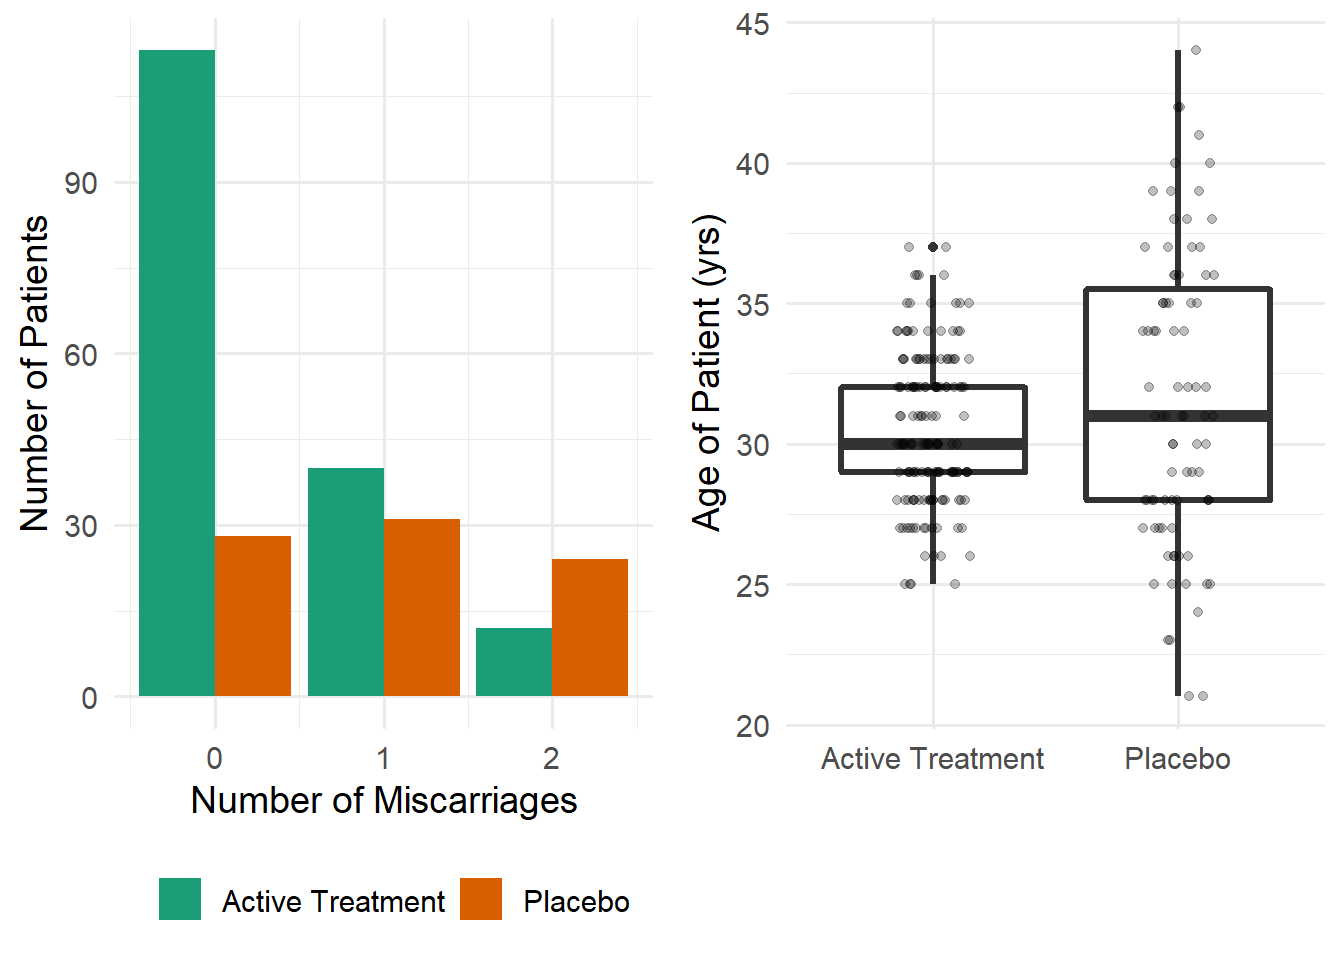
\includegraphics[width=0.8\textwidth]{./Images/statistical-process-graphics-1} 

}

\caption{Two graphical presentations of data from a hypothetical study, adhering to good graphical practices.}\label{fig:statistical-process-graphics}
\end{figure}

Notice that the left panel of the graphic makes use of bar charts to compare a qualitative variable (number of miscarriages) across a second qualitative variable (treatment group). The use of color here is important because it brings out additional features which do not appear on the x- or y-axis. The right panel of the graphic makes use of box-plots (with jitter-plots overlayed) to compare a quantitative variable (age of the patient) across the qualitative variable (treatment group). One idea worth discussing here is that a graphical summary of a quantitative variable should always portray both \emph{location} and \emph{spread}. Notice that in the right panel in Figure \ref{fig:statistical-process-graphics}, we see that the age of the patients receiving placebo is comparable to that of those receiving the active treatment; however, the variability in the ages of patients receiving placebo is much larger compared to those receiving the active treatment. Compare this to Figure \ref{fig:statistical-process-poor-graphics}, which only summarizes location with no sense of spread; while this is a popular default graphic in some software, it does not adequately allow a reader to determine the size of the effect relative to the variability in the data.

\begin{figure}

{\centering 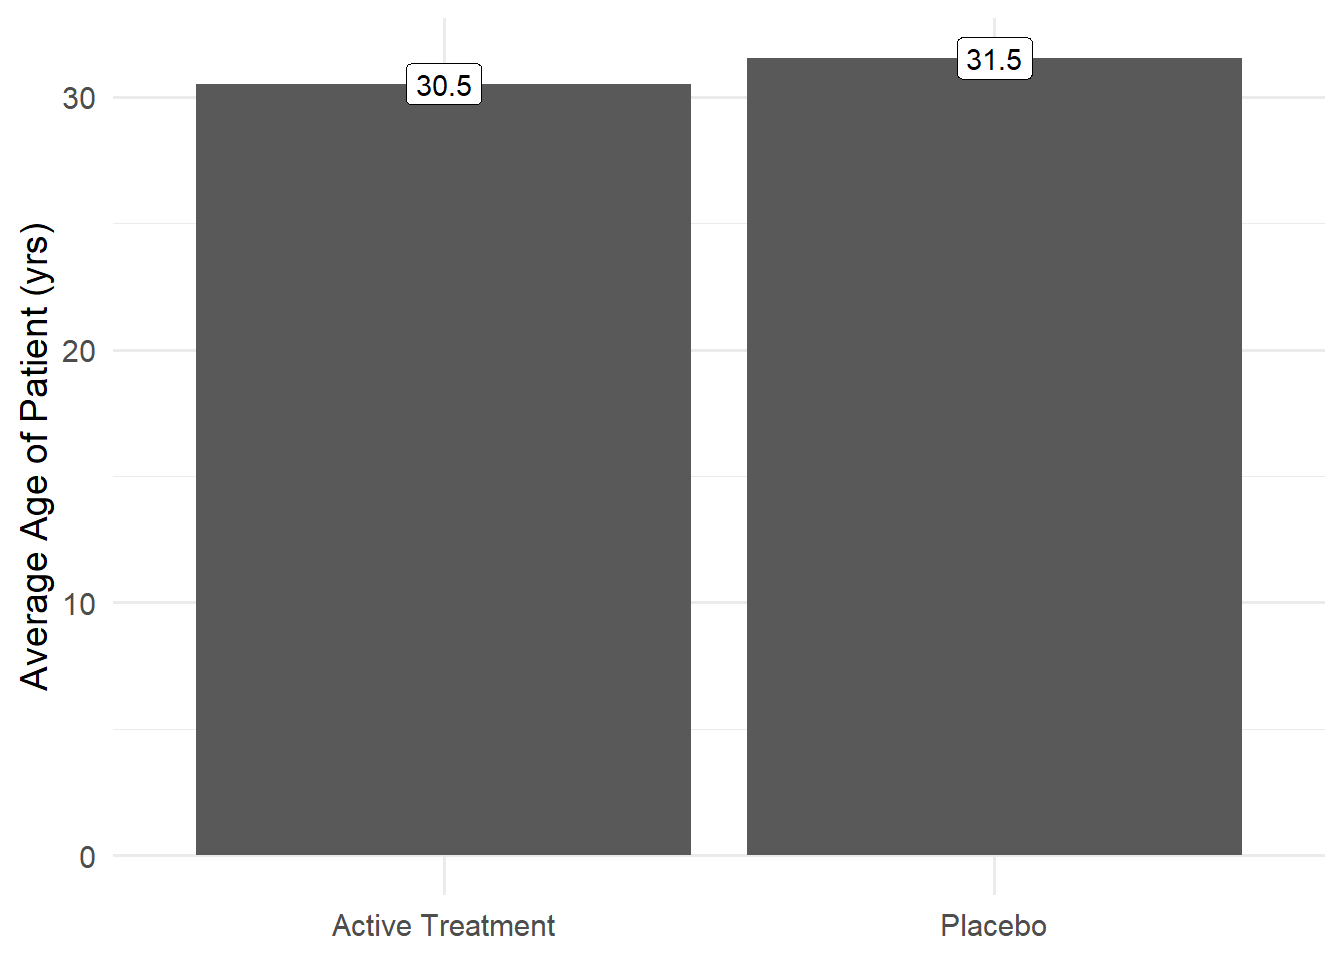
\includegraphics[width=0.8\textwidth]{./Images/statistical-process-poor-graphics-1} 

}

\caption{Inappropriate graphical presentation from a hypothetical study as it ignores a sense of variability in the data.}\label{fig:statistical-process-poor-graphics}
\end{figure}

\hypertarget{basic-terminology-for-statistical-tests}{%
\section{Basic Terminology for Statistical Tests}\label{basic-terminology-for-statistical-tests}}

In some cases, summarizing the data numerically and graphically is sufficient for telling a compelling story. Often, however, the summaries are accompanied by a statistical analysis. Regardless of the simplicity (or complexity) of the statistical procedure, there are a few fundamental ideas which are common to all methods.

A \textbf{statistic} (summary of data) is a point estimate of a \textbf{parameter} (corresponding value in the population of interest). For example, the value 0.39 in Table \ref{tab:statistical-process-data-summary} is the average number of miscarriages among those women in the study who received the active treatment; but, it \emph{estimates} the average number of miscarriages among all women if they were to receive the active treatment.

\begin{definition}[Parameter]
Numeric quantity which summarizes the distribution of a variable within the \emph{population} of interest. Generally denoted by Greek letters in statistical formulas.
\end{definition}

\begin{definition}[Statistic]
Numeric quantity which summarizes the distribution of a variable within the observed \emph{sample}.
\end{definition}

Instead of estimating a parameter with this single value, we can estimate the parameter with a \textbf{confidence interval} (a 95\% confidence interval is standard practice).

\begin{definition}[Confidence Interval]
An interval (range of values) estimate of a parameter that incorporates the variability in the statistic. The process of constructing \(k\)\% confidence intervals results in them containing the parameter of interest in \(k\)\% of repeated studies. The value of \(k\) is called the \emph{confidence level}.
\end{definition}

It is important to recognize that the entire interval is our estimate. In text, we generally report the point estimate with the 95\% confidence interval in parentheses. For example,

\begin{quote}
The probability of a miscarriage is 0.32 (95\% CI: {[}0.25, 0.39{]}) for women given the active treatment.
\end{quote}

There are several common misinterpretations of a confidence interval; generally, these do not enter the literature because we avoid interpreting the interval directly and simply state it and discuss its implications (as above). For completeness, however, it is best to think of a confidence interval as giving all the reasonable values of the parameter based on the data observed.

While confidence intervals estimate an effect, a \textbf{p-value} quantifies the amount of evidence in the data against the lack of an effect.

\begin{definition}[P-Value]
The probability, assuming the null hypothesis is true, that we would observe a statistic, from sampling variability alone, as extreme or more so as that observed in our sample. This quantifies the strength of evidence against the null hypothesis. Smaller values indicate stronger evidence.
\end{definition}

We generally report a p-value to 3 decimal places (with values less than 0.001 being written as ``\textless{} 0.001''). It is best to state p-values alongside the conclusion. For example,

\begin{quote}
There is strong evidence (p \textless{} 0.001) that the active treatment reduces the risk of a miscarriage.
\end{quote}

There are two very important things to keep in mind when examining a p-value:

\begin{enumerate}
\def\labelenumi{\arabic{enumi}.}
\tightlist
\item
  A small p-value does not imply the effect is clinically important. It simply indicates that we are able to statistically discern an effect is present.
\item
  A large p-value does not imply there is no effect. It simply indicates that we cannot statistically discern the presence of an effect.
\end{enumerate}

For these reasons, a p-value should always be accompanied by either a confidence interval (preferred when possible) or a point estimate of the effect to allow readers to determine if the impact is clinically important.

When interpreting statistical results, the design of the study plays a role. In particular, we can only conclude a causal relationship when the data is from a \textbf{randomized clinical trial}. When your data is from an \textbf{observational study}, any group comparisons are subject to \textbf{confounding}.

\begin{definition}[Randomized Clinical Trial]
Also called a ``controlled experiment,'' a study in which each subject is randomly assigned to one of the groups being compared in the study.
\end{definition}

\begin{definition}[Observational Study]
A study in which each subject ``self-selects'' into one of groups being compared in the study. The phrase ``self-selects'' is used very loosely here and can include studies in which the groups are defined by an inherent characteristic or the groups are chosen haphazardly.
\end{definition}

\begin{definition}[Confounding]
When the effect of a variable on the response is mis-represented due to the presence of a third, potentially unobserved, variable known as a confounder.
\end{definition}

As an example, it has been suggested that brushing your teeth twice a day for at least two minutes may lower the risk of cardiovascular diseases\footnote{\url{https://www.heart.org/en/news/2018/11/07/bad-tooth-brushing-habits-tied-to-higher-heart-risk}}. However, most of these results are from large surveys, which are observational studies. It is quite plausible that those who take excellent care of their teeth tend to be health-conscious individuals, and health-conscious individuals are more likely to have healthy diets and exercise regularly, both of which decrease the risk of cardiovascular diseases. In this example, being health-conscious is a confounder because it is associated with \emph{both} the factor under study (brushing behavior) \emph{and} the outcome of interest (cardiovascular disease); see Figure \ref{fig:statistical-process-confounding}. In order to establish a causal link between brushing and the risk of cardiovascular disease, we could conduct a clinical trial in which we randomize patients to a brushing routine and then track their long-term cardiovascular health; then, the link between the confounder and the treatment group is broken, allowing us to make a causal conclusion. While clinical trials allow for causal conclusions, they are not always feasible or practical; observational studies allow us to add to the body of knowledge in such situations. There are some methods for addressing confounding in observational studies through statistical analysis, but such methods often require a large sample and more advanced methodology.

\begin{figure}

{\centering 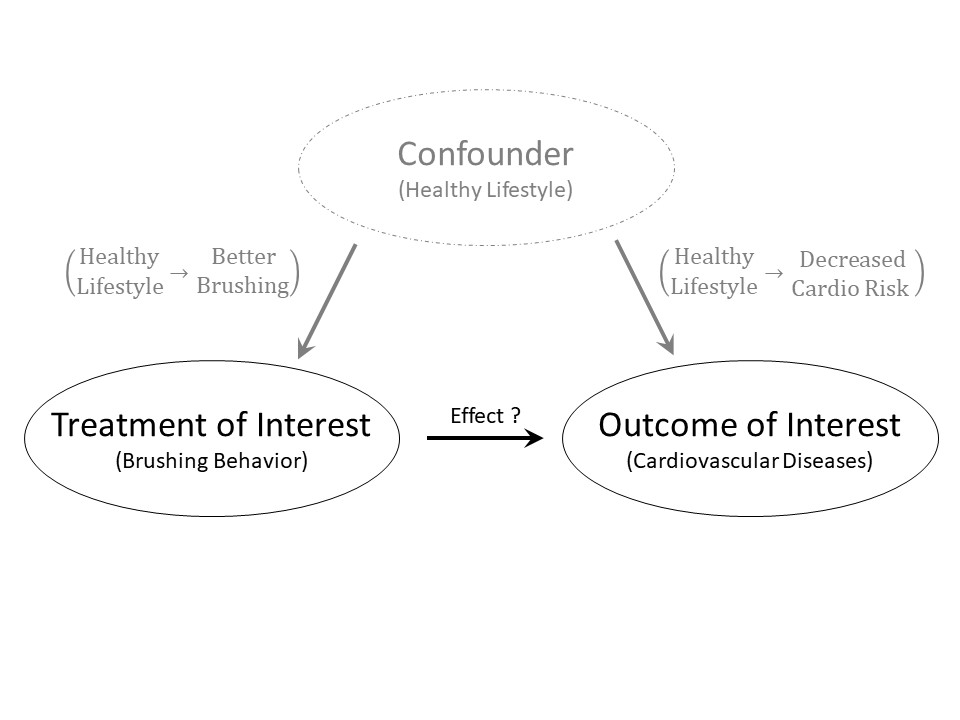
\includegraphics[width=0.8\textwidth]{images/Statistical-Process-Confounding} 

}

\caption{Illustration of confounding in observational studies.}\label{fig:statistical-process-confounding}
\end{figure}

\hypertarget{a-note-on-codebooks}{%
\section{A Note on Codebooks}\label{a-note-on-codebooks}}

A dataset on its own is meaningless if you cannot understand what the values represent. \emph{Before} you access a dataset, you should always review any available \textbf{codebooks}.

\begin{definition}[Codebook]
Also called a ``data dictionary,'' these provide complete information regarding the variables contained within a dataset.
\end{definition}

Some codebooks are excellent, with detailed descriptions of how the variables were collected and appropriate units. Other codebooks give only an indication of what each variable represents. Whenever you are working with previously collected data, reviewing a codebook is the first step; and, you should be prepared to revisit the codebook often throughout an analysis. When you are collecting your own dataset, constructing a codebook is essential for others to make use of your data.

\hypertarget{distributional-quartet}{%
\chapter{Distributional Quartet}\label{distributional-quartet}}

Any good statistical analysis moves between four key distributions --- what we refer to as the \emph{Distributional Quartet}. While not always explicitly discussed, these distributions are always present in an analysis. Understanding their role is important to implementing and interpreting the various components of an analysis.

We begin by considering the following example from Rosner (\protect\hyperlink{ref-Rosner2006}{2006}).

\begin{example}[Blood Pressure when Lying Down]
\protect\hypertarget{exm:distributional-quartet-bp}{}\label{exm:distributional-quartet-bp}Blood pressure is one measure for the health of your heart. A blood pressure reading includes two numbers --- the systolic blood pressure (the ``top number,'' measures the amount of pressure in your arteries when your heart contracts) and the diastolic blood pressure (the ``bottom number,'' measures the amount of pressure in your arteries when your heart is between beats). However, an individual does not have a single blood pressure reading; our blood pressure fluctuates as a result of activity as well as our position. In a study examining the impact of position on blood pressure, 32 participants had their blood pressure measured while lying down with their arms at their sides.
\end{example}

Stated simply, the discipline of statistics is about using data to say something about a process that characterizes a population. Our analysis, therefore, begins with the \textbf{Distribution of the Population}.

\begin{rmdfivefund}
\textbf{Distribution of Population}: The pattern of variability in values of a variable across individuals of the population. The shape of this distribution is governed by unknown parameters. While we generally do not know the shape of this distribution, we may occasionally posit a model for it.
\end{rmdfivefund}

We are interested in using the data from this study to characterize the systolic blood pressure of individuals when in this recumbent position, with their arm at their side. Of course, we are unable to assess the blood pressure of all individuals in the world. Therefore, we do not know what the distribution of systolic blood pressure measurements is for this population. However, we \emph{might} posit a model for this distribution. Such models, which must account for the variability among the population, are studied in probability theory, which we consider in the next section. For now, it suffices to imagine the distribution of the population graphically; it is characterized by the unknown parameters (Figure \ref{fig:distributional-quartet-population}).

\begin{figure}

{\centering 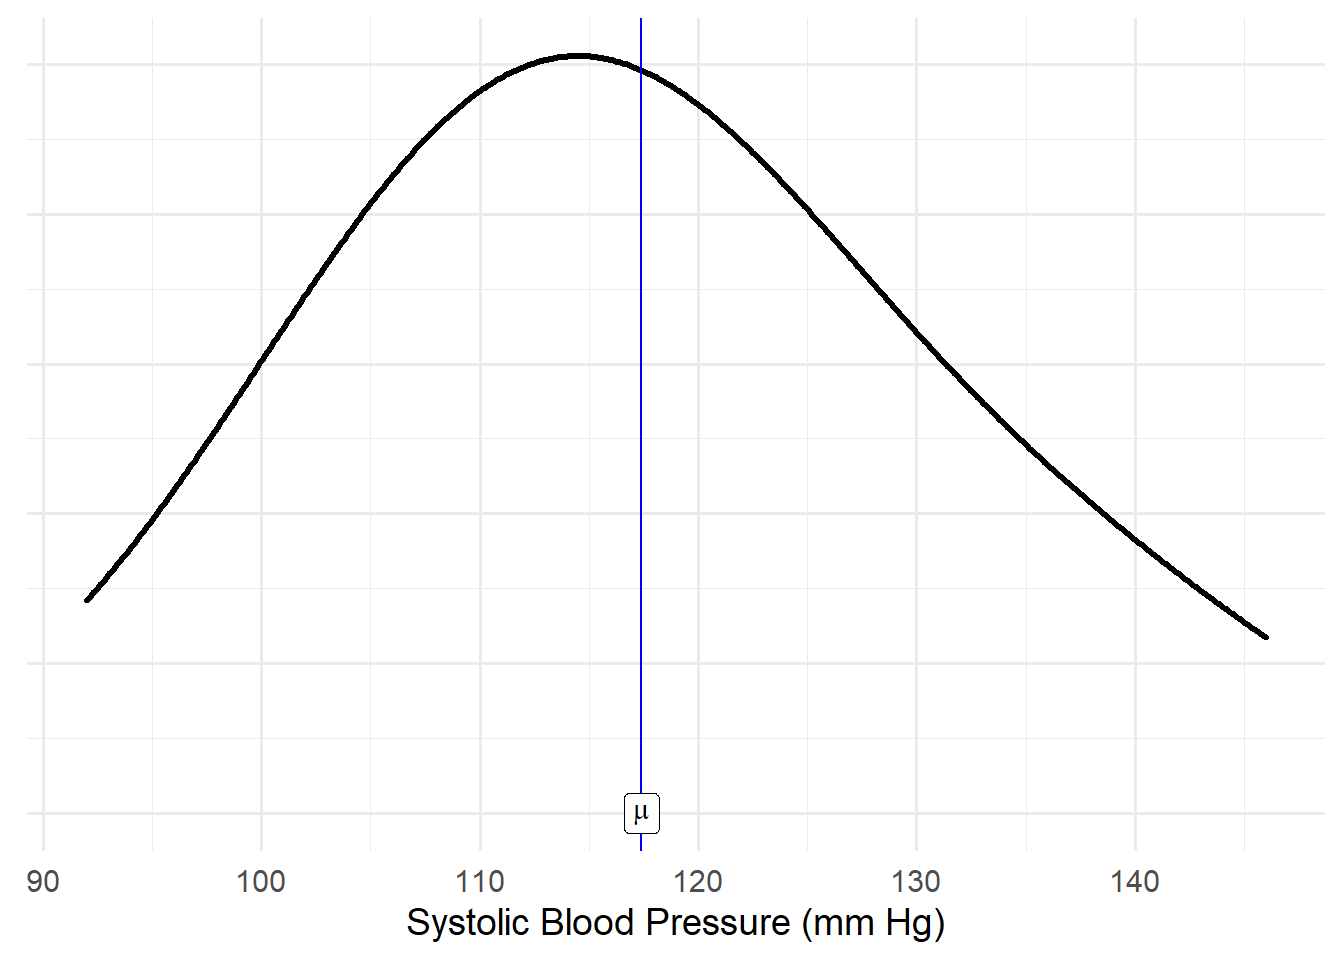
\includegraphics[width=0.8\textwidth]{./Images/distributional-quartet-population-1} 

}

\caption{Hypothetical model for the distribution of systolic blood pressure within the population. The unknown population is denoted on the graphic.}\label{fig:distributional-quartet-population}
\end{figure}

The data we actually observe comes from the sample, and we will use this smaller group to say something about the underlying population. It is the distribution of sample which we are summarizing each time we construct a graphic.

\begin{rmdfivefund}
\textbf{Distribution of Sample}: The pattern of variability in values of a variable across individuals of the sample. This is typically summarized graphically and numerically.
\end{rmdfivefund}

Figure \ref{fig:distributional-quartet-sample} summarizes the sample using a histogram. If our sample is collected well, then it should be representative of the population, meaning that the distribution of the sample should reflect the characteristics of the (unobserved) distribution of the population. The location, spread, and shape should all reflect what we might see within the population.

\begin{figure}

{\centering 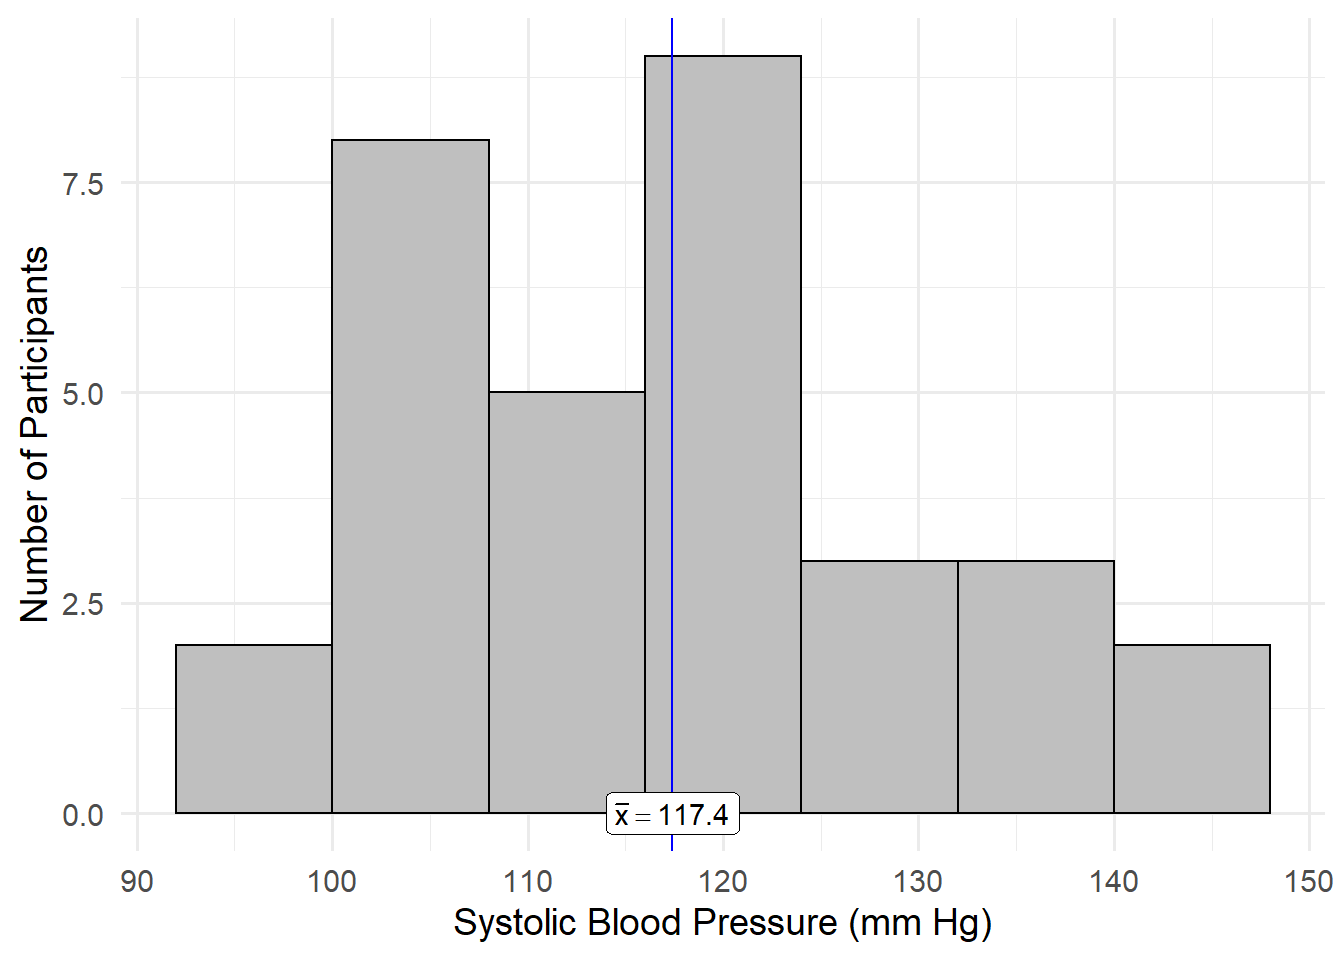
\includegraphics[width=0.8\textwidth]{./Images/distributional-quartet-sample-1} 

}

\caption{Distribution of systolic blood pressure within the sample of 32 participants.}\label{fig:distributional-quartet-sample}
\end{figure}

Examining the sample is critical to understanding the story in the data. However, the sample alone does not allow us to make inference. We must remember that the statistics we compute using our sample are dependent upon the data we observed. If we were to repeat the sampling process (collect new data to answer the same question), our statistics would change. Inference requires us to acknowledge the sampling variability and incorporate it when making statements about the population.

\begin{rmdfivefund}
\textbf{Sampling Distribution}: The pattern of variability in values of a \emph{statistic} (or standardized statistic) across repeated samples of the same size from the population. This must be modeled in practice.
\end{rmdfivefund}

As we are generally unable to perform replicate studies, we model the sampling distribution using the data available (future chapters will discuss the various methods available for modeling this distribution). The model allows us to determine values of the parameter for which the data is consistent. That is, it allows us to compute a confidence interval to estimate a parameter of interest. For example, a 95\% CI for the mean systolic blood pressure (mm Hg, when recumbent with arm at their side), based on our data available, is (113.1, 121.9); this is illustrated in Figure \ref{fig:distributional-quartet-sampling-distribution} alongside the model for the sampling distribution of the sample mean systolic blood pressure from which the CI was computed.

\textbackslash begin\{figure\}

\{\centering 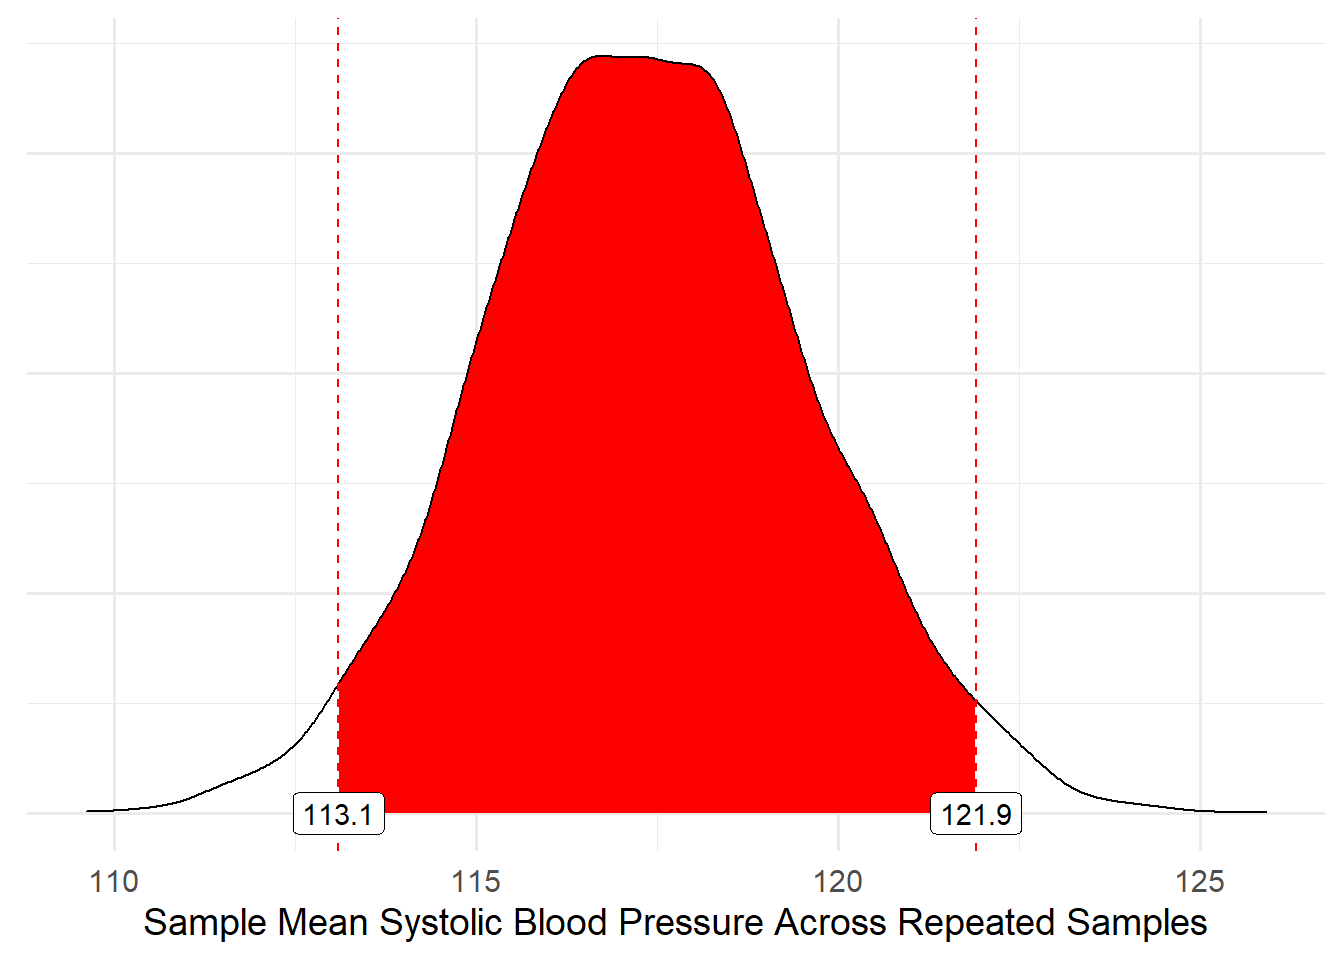
\includegraphics[width=0.8\textwidth]{./Images/distributional-quartet-sampling-distribution-1}

\}

\textbackslash caption\{Empirical model for the sampling distribution of mean systolic blood pressure within the sample of 32 participants. A 95\% confidence interval is also illustrated.\}\label{fig:distributional-quartet-sampling-distribution}
\textbackslash end\{figure\}

While statisticians generally have a preference toward estimation (and therefore reporting confidence intervals), scientists often have specific research questions they would like to address. When this is the case, the scientist may want to quantify the strength of evidence in the sample against some specified hypothesis. In order to determine how rare our data is, we must know what we should expect under the specified hypothesis.

\begin{rmdfivefund}
\textbf{Null Distribution}: The sampling distribution of a statistic (or standardized ``test'' statistic) \emph{when the null hypothesis is true}. This must be modeled in practice.
\end{rmdfivefund}

The null distribution effectively tells us what values of the statistic we would expect to see if the null hypothesis were true. If our observed statistic then seems plausible according to the null distribution, then the null hypothesis is reasonable. If, on the other hand, our observed statistic is unexpected according to the null distribution, then we have evidence that the null hypothesis is false (and therefore that the alternative is true). Note that these are our only two potential conclusions. This evidence is quantified by the p-value. For example, suppose we are interested in using our data to test the following set of hypotheses:

\[H_0: \mu = 120 \qquad \text{vs.} \qquad H_1: \mu \neq 120.\]

That is, we are interested in determining if there is evidence that, on average, the systolic blood pressure (recumbent with arm at side) differs from 120 mm Hg. According to the data, it is reasonable (p = 0.247) that the average systolic blood pressure is 120 mm Hg. The computation of the p-value is illustrated in Figure \ref{fig:distributional-quartet-null-distribution} alongside the model for the null distribution for this particular hypothesis.

\begin{figure}

{\centering 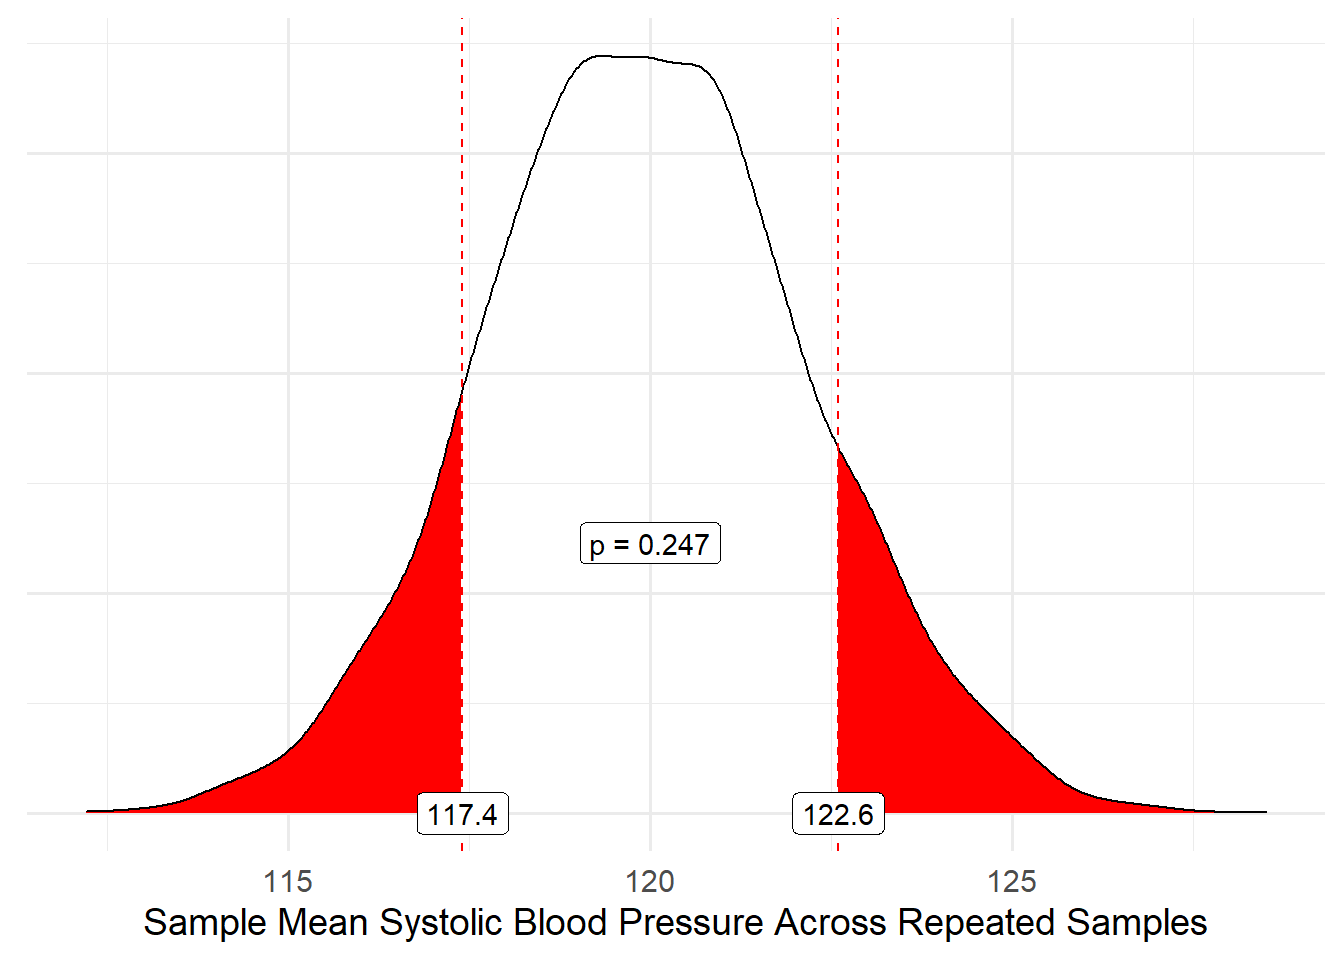
\includegraphics[width=0.8\textwidth]{./Images/distributional-quartet-null-distribution-1} 

}

\caption{Empirical model for the null distribution of mean systolic blood pressure within the sample of 32 participants when the null hypothesis is that the mean systolic blood pressure is 120 mm Hg. The p-value is also illustrated.}\label{fig:distributional-quartet-null-distribution}
\end{figure}

Our focus in this short review is not this specific analysis. The emphasis here is on the \emph{process\}} --- the use of the four distributions used in a statistical analysis. They allow us to use the sample to make inference on the underlying population. As we move forward in the course, we will study more sophisticated models. However, behind the scenes, the procedures are always bouncing between these four distributions in order to allow us to make inference.

\hypertarget{essential-probability}{%
\chapter{Essential Probability}\label{essential-probability}}

Statistics uses data to make inference on a population. In turn, statistical theory is built on probability --- the discipline of mathematics which studies and models random processes. While we do not need a thorough mastery of probability to be practitioners of statistical methodology, a foundation in probability models is helpful for seeing common threads in statistical modeling. This chapter provides a brief introduction to the most relevant aspects of probability theory necessary for engaging with the remainder of the text.

\hypertarget{density-functions-as-models}{%
\section{Density Functions as Models}\label{density-functions-as-models}}

Any process for which the outcome cannot be predicted with certainty is a random process. Typically, probability is taught from a mathematical perspective, with a goal of constructing a coherent and complete framework for characterizing such processes. Here, our goal is to introduce key probability concepts by relating them to their data-centric analogues. That is, we want to think of probability in light of how we will use it in statistical analysis.

Each time we collect data, we can think of each observation as the result of a random process. These observations are recorded as variables in our dataset. In probability, a random variable is used to represent a measurement that results from a random process. Just as we have both \emph{quantitative} and \emph{qualitative} variables, there are \emph{continuous} and \emph{discrete} random variables.

\begin{definition}[Random Variable]
Represents a measurement that will be collected and for which the value cannot be predicted with certainty. Generally represented with a capital letter. Continuous random variables represent quantitative measurements while discrete random variables represent qualitative measurements.
\end{definition}

Consider measuring a single variable on a sample of \(n\) subjects. Then, we might represent the measurements we will obtain as \(X_1, X_2, \dots, X_n\).

\begin{rmdtip}
There are many ways to interpret probability. In classical (``frequentist'') statistics, we think of probability as the likelihood of an event in repeated experimentation. Therefore, probability does not describe events that have already occured; we can only describe future events.\\
\end{rmdtip}

Each of our random variables \(X_1, X_2, \dotsc, X_n\) will be observations from some underlying population. As we described in previous chapters, the population is unknown. However, we might posit a model for its distribution. This is our primary use of probability theory in statistics --- to model distributions. The most common way to represent a probability model is through its density function.

\begin{definition}[Density Function]
A density function \(f\) relates the potential values of a random variable \(X\) with the probability those values occur. For a \emph{continuous} random variable, the probability the random variable \(X\) falls within an interval \((a, b)\) is given by

\[Pr(a \leq X \leq b) = \int_{a}^{b} f(x) dx.\]

For a \emph{discrete} random variable, the probability the random variable \(X\) is equal to the value \(u\) is given by

\[Pr(X = u) = f(u).\]
\end{definition}

\begin{rmdtip}
In a probability course, there is often a distinction made between probability density functions (continuous random variables) and probability mass functions (discrete random variables). We do not make this distinction and instead rely on the context to determine whether we are dealing with a continuous or discrete random variable.
\end{rmdtip}

With few exceptions, we will be working with continuous random variables. As a result, the density function is a smooth function over some region, and the actual value of the function is not interpretable; instead, we get at a probability by considering the area under the curve. Again, drawing connections to data analysis, we can think of a density function as a mathematical formula representing a smooth histogram. The area under the curve for any region gives the proportion of the population which has a value in that region. That is, we get the probability that a random variable will be in an interval by integrating the density function over that interval. Figure \ref{fig:essential-probability-density} illustrates this idea; we have a hypothetical dataset which has been summarized using a histogram; we overlay a density function (with the corresponding mathematical model that describes this density function). The figure shows how the sample (summarized in the histogram) is approximating the population (the density function).

\begin{figure}

{\centering 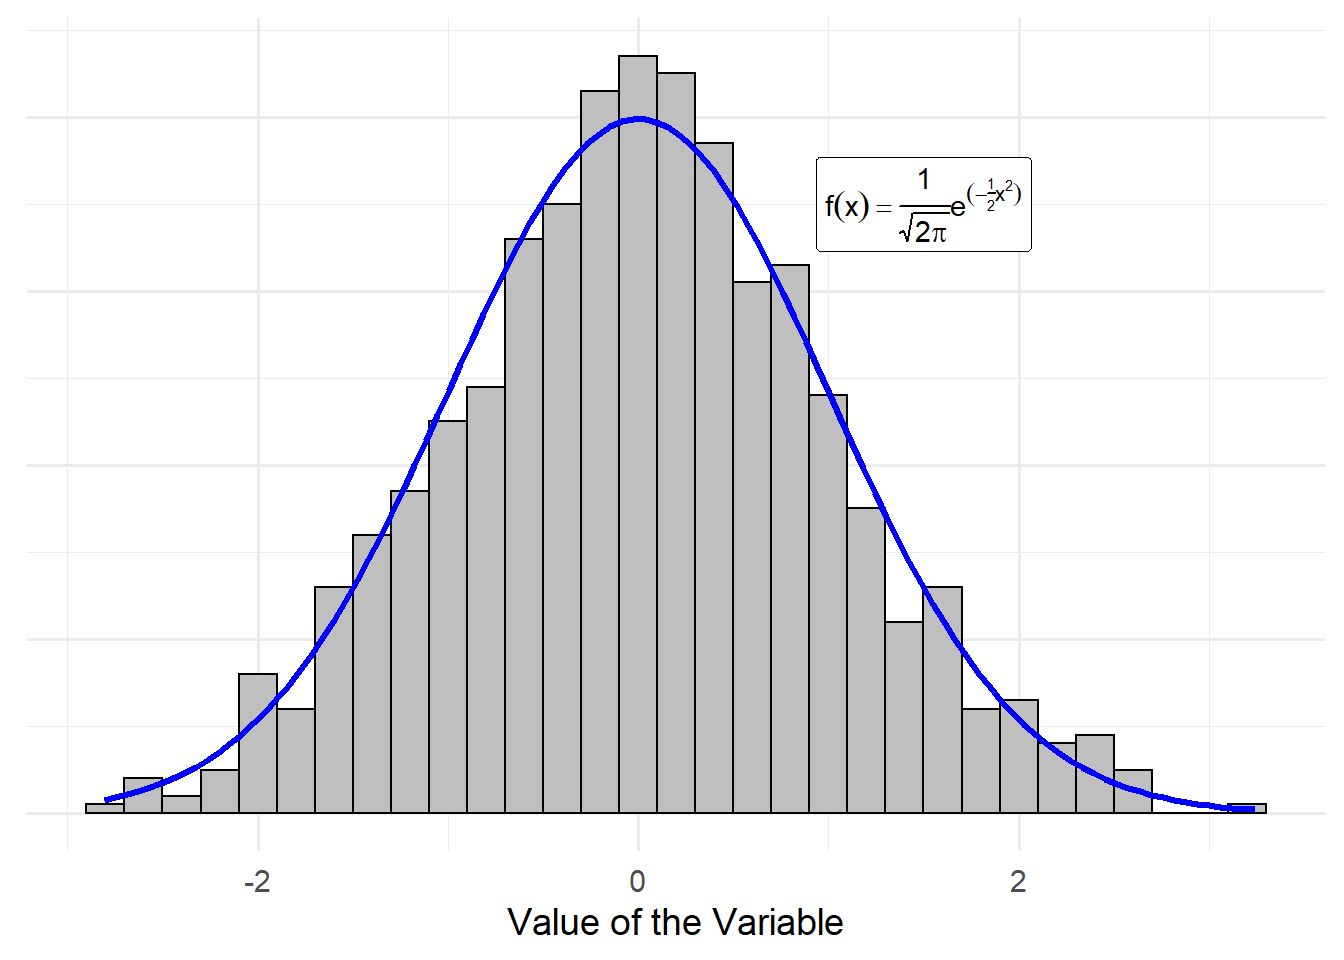
\includegraphics[width=0.8\textwidth]{./Images/essential-probability-density-1} 

}

\caption{Illustration of a density function representing the distribution of the population and a histogram from a representative sample.}\label{fig:essential-probability-density}
\end{figure}

Especially for visualization, the density function is the most common way of characterizing a probability model. However, computing the probability using the density is problematic due to the integration required. Many software address this by working with the cumulative distribution function (CDF).

\begin{definition}[Cumulative Distribution Function (CDF)]
Let \(X\) be a random variable; the cumulative distribution function (CDF) is defined as

\[F(u) = Pr(X \leq u).\]

For a continuous random variable, we have that

\[F(u) = \int_{-\infty}^{u} f(x) dx\]

implying that the density function is the derivative of the CDF. For a discrete random variable

\[F(u) = \sum_{x \leq u} f(x).\]
\end{definition}

Working with the CDF improves computation because it avoids the need to integrate each time; instead, the integral is computed once (and stored internally in the computer) and we use the result to compute probabilities directly.

\begin{rmdkeyidea}
Density functions are the mathematical models for distributions; they link values of the variable with the likelihood of occurence. However, for computational reasons, we often work with the cumulative distribution function which provides the probability of being less than or equal to a value.
\end{rmdkeyidea}

\hypertarget{summarizing-distributions-parameters}{%
\section{Summarizing Distributions (Parameters)}\label{summarizing-distributions-parameters}}

Most scientific questions are focused on the location or spread of a distribution. For example, we are interested in estimating the average yield of a crop, or the variance in the amount of sleep among college students. Introductory statistics introduces summaries of location and spread within the sample (e.g., sample mean for location and sample variance for spread). Analogous summaries exist for density functions.

In particular, the mean of a random variable (denoted by \(E(X)\)) and the variance of a random variable (denoted by \(Var(X)\)) are measures of the location and spread, respectively, of the distribution represented by its corresponding density function. When the density function is a model for the population, these represent the parameters of the population --- the same parameters we estimate and make inference on using our data analysis. For completeness, we present the computational formulas for the mean and variance of a random variable, but we do not make use of these formulas moving forward. Instead, we simply note that these formulas are similar to their sample counterparts.

\begin{definition}[Mean and Variance of a Random Variable]
Suppose \(X\) is a random variable with density function \(f\). If \(X\) is a continuous random variable, then the mean and variance are given by

\[
\begin{aligned}
  E(X) &= \int x f(x) dx \\
  Var(X) &= \int \left(x - E(X)\right)^2 f(x) dx.
\end{aligned}
\]

If \(X\) is a discrete random variable, then the mean and variance are given by

\[
\begin{aligned}
  E(X) &= \sum x f(x) \\
  Var(X) &= \sum \left(x - E(X)\right)^2 f(x).
\end{aligned}
\]
\end{definition}

As we have stated, the distribution of the population is generally unknown. If we were able to specify the density function for the population, then there would be no need for statistical analysis. Instead, the model is generally posited up to some unknown values (parameters). For example, a researcher might posit that within the population, the time until a medical device fails could be modeled using the density

\[f(x) = \frac{1}{\mu} e^{-\frac{x}{\mu}} \qquad x > 0.\]

Here, the researcher has really posited a form of the model, but not the exact model. The value \(\mu\) is the average (which could be confirmed using the formulas in the above definition). In such cases, making inference on the parameters allows us to really characterize the entire distribution of the population.

\begin{rmdkeyidea}
When a probability model is specified for a population, it is generally specified up to some unknown parameter(s). Making inference on the unknown parameter(s) therefore characterizes the entire distribution.
\end{rmdkeyidea}

\hypertarget{specific-models-for-populations}{%
\section{Specific Models for Populations}\label{specific-models-for-populations}}

While we could posit any non-negative function as a model for a density function, there are some models that are very common. The most common model for the population of a continuous random variable is the Normal distribution.

\begin{definition}[Normal (Guassian) Distribution]
Let \(X\) be a continuous random variable. \(X\) is said to have a Normal (or Guassian) distribution if the density is given by

\[f(x) = \frac{1}{\sqrt{2 \pi \sigma^2}} e^{-\frac{1}{2\sigma^2} (x - \mu)^2} \qquad -\infty < x < \infty,\]

where \(\mu\) is any real number and \(\sigma^2 > 0\).

\begin{itemize}
\tightlist
\item
  \(E(X) = \mu\)
\item
  \(Var(X) = \sigma^2\)
\end{itemize}

We write \(X \sim N\left(\mu, \sigma^2\right)\), which is read ``X has a Normal distribution with mean \(\mu\) and variance \(\sigma^2\).'' This short-hand implies the density above.
\end{definition}

This model is a bell-shaped distribution centered at the mean \(\mu\). While this is a common model, it should not be assumed by default. In future chapters, we will consider methods for assessing whether assuming a Normal distribution is reasonable.

When a response is binary (assumes one of two values), it is a Bernoulli distribution. In order to make use of this distribution, we typically define one of the two possible outcomes as a ``success'' and the other as a ``failure.'' For example,

\[X = \begin{cases} 1 & \text{if a success is observed} \\ 0 & \text{if a success is not observed} \end{cases}.\]

\begin{definition}[Bernoulli Distribution]
Let \(X\) be a discrete random variable taking the value 0 or 1. \(X\) is said to have a Bernoulli distribution with density

\[f(x) = \theta^x (1 - \theta)^(1 - x) \qquad x \in \{0, 1\},\]

where \(0 < \theta < 1\) is the probability that \(X\) takes the value 1.

\begin{itemize}
\tightlist
\item
  \(E(X) = \theta\)
\item
  \(Var(X) = \theta(1 - \theta)\)
\end{itemize}

We write \(X \sim Ber(\theta)\), which is read ``X has a Bernoulli distribution with probability \(\theta\).''
\end{definition}

\begin{rmdtip}
A generalization of the Bernoulli distribution is the Binomial distribution. So, we sometimes hear people refer to a Bernoulli distribution as ``a Binomial distribution with a single event.''
\end{rmdtip}

\hypertarget{models-for-sampling-distributions-and-null-distributions}{%
\section{Models for Sampling Distributions and Null Distributions}\label{models-for-sampling-distributions-and-null-distributions}}

A statistical analysis does not exist in a vacuum. Instead, based on the context of the study, we make assumptions about the process which generated the data. The conditions we are willing to assume govern how we model the sampling distribution or null distribution. Occasionally, we can lean on statistical theory to say how the sampling distribution or null distribution will behave. That is, under certain conditions, statistical theory tells us what the appropriate model is. In these situations, there are some common models.

The t-distribution is a bell-shaped distribution, similar to the Normal distribution but with wider tails. It has a single parameter, known as the degrees of freedom. Note that unlike many other distributions, this parameter (the degrees of freedom) are not associated with the location of the distribution. Instead, they govern the spread (but are not the variance).

\begin{definition}[t-Distribution]
Let \(X\) be a continuous random variable. \(X\) is said to have a t-distribution if the density is given by

\[f(x) = \frac{\Gamma \left(\frac{\nu+1}{2} \right)} {\sqrt{\nu\pi}\,\Gamma \left(\frac{\nu}{2} \right)} \left(1+\frac{x^2}{\nu} \right)^{-\frac{\nu+1}{2}} \qquad x > 0\]

where \(\nu > 0\) is the degrees of freedom.

We write \(X \sim t_{\nu}\), which is read ``X has a t-distribution with \(\nu\) degrees of freedom.''
\end{definition}

The Chi-Square distribution is a skewed distribution (looks like a giant slide). It has a single parameter, known as the degrees of freedom. The degrees of freedom for this distribution characterize both the location and spread simultaneously.

\begin{definition}[Chi-Square Distribution]
Let \(X\) be a continuous random variable. \(X\) is said to have a Chi-Square distribution if the density is given by

\[f(x) = \frac{1}{2^{\nu/2}\Gamma (\nu/2)}\;x^{\nu/2-1}e^{-x/2} \qquad x > 0,\]

where \(\nu > 0\) is the degrees of freedom.

We write \(X \sim \chi^2_{\nu}\), which is read ``X has a Chi-Square distribution with \(\nu\) degrees of freedom.''
\end{definition}

The F-distribution is a skewed distribution. It has two parameters, known as the numerator and denominator degrees of freedom. While neither variable is directly the mean and variance, together these two parameters characterize both the location and the spread.

\begin{definition}[F-Distribution]
Let \(X\) be a continuous random variable. \(X\) is said to have an F-distribution if the density is given by

\[f(x) = \frac{\Gamma((r + s)/2)}{(\Gamma(r/2) \Gamma(s/2))} (r/s)^{(r/2)} x^{(r/2 - 1)} (1 + (r/s) x)^{-(r + s)/2} \qquad x > 0,\]

where \(r,s > 0\) are the numerator and denominator degrees of freedom, respectively.

We write \(X \sim F_{r, s}\), which is read ``X has an F-distribution with r numerator degrees of freedom and s denominator degrees of freedom.''
\end{definition}

\begin{figure}

{\centering 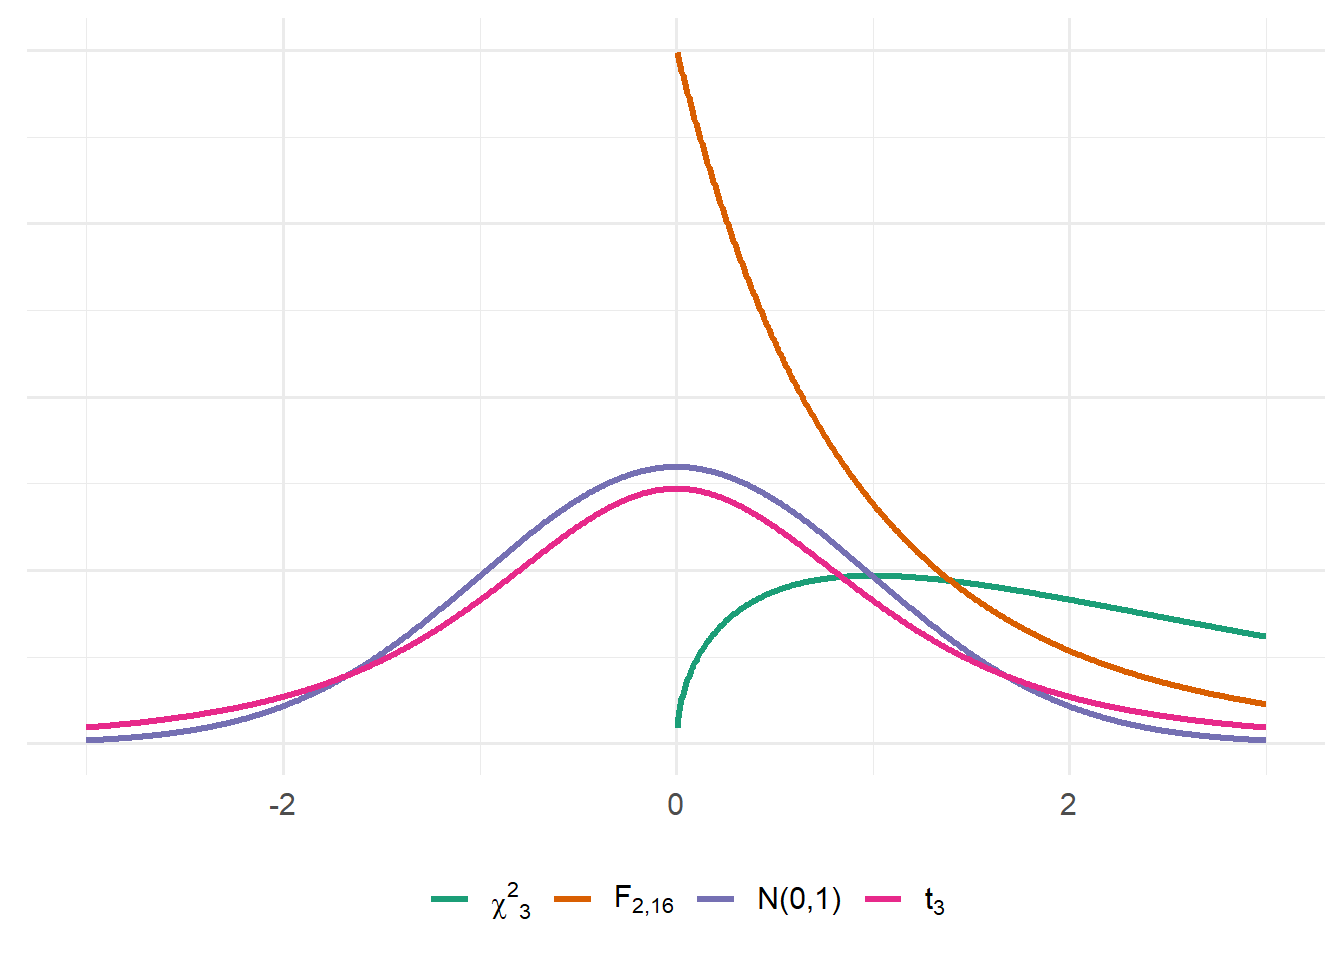
\includegraphics[width=0.8\textwidth]{./Images/essential-probability-comparisons-1} 

}

\caption{Comparison of various common distributions.}\label{fig:essential-probability-comparisons}
\end{figure}

The formulas above are ugly, but we will not be working with them directly. Instead, statistical software have these distributions embedded. The key idea here is that when we know the model for a sampling distribution, we are able to rely on that model in order to obtain confidence intervals. And, when we have a model for the null distribution, we are able to rely on that model to obtain p-values. These models are what underlies many default implementations of statistical methods in software.

\begin{rmdkeyidea}
Some probability models occur so frequently that we give them names for easy reference. Some models are common for modeling the population, in which case they are defined in terms of unknown parameters to be estimated. Some models are common for modeling sampling distributions or null distributions, in which case their form will be explicitly determined according to statistical theory.
\end{rmdkeyidea}

\hypertarget{part-general-linear-model-and-modeling-strategies}{%
\part{General Linear Model and Modeling Strategies}\label{part-general-linear-model-and-modeling-strategies}}

\hypertarget{glm-framework}{%
\chapter{General Linear Model Framework}\label{glm-framework}}

The general linear model, also known as multiple linear regression, provides a framework appropriate for modeling a continuous outcome (response) as a function of several predictors. This framework unifies the methods discussed in a typical introductory course. After introducing the framework, we use this platform to introduce several flexible modeling strategies helpful when addressing common scientific questions.

The development of a model should not be divorced from its intended use, and in general, there are three uses for multivariable models. That is, the majority of scientific questions can be categorized into one of three groups: prediction, isolating an effect, or studying the interplay between variables.

\begin{rmdkeyidea}
There are primarily three uses for a multivariable model

\begin{itemize}
\tightlist
\item
  \textbf{Prediction}: modeling a relationship for the purpose of estimating a future occurence given new data.
\item
  \textbf{Isolating an Effect}: describing the relationship between a response and predictor after accounting for the influence of other predictors measured.
\item
  \textbf{Studying the Interplay}: examining how the relationship of two variables is impacted by the value of a third variable.
\end{itemize}
\end{rmdkeyidea}

While we introduce these elements in the context of the general linear model, note that these uses carry over into other regression models we will examine.

Consider a gardener studying two common organic fertilizers. She could have the following questions in mind:

A. What do I anticipate the yield of tomatoes to be next summer when using cow manure?
B. Does bat guano tend to result in higher tomato yields compared with cow manure after accounting for any differences in yield due to the amount of water the plants receive?
C. Does the efficacy of bat guano (compared with cow manure) depend on the amount of sunlight the plants receive?

The first question is an example of predicting; given the fertilizer being considered (as well as potentially other characteristics of the garden), what does she expect the results to be in the future? The second question examines the impact (or effect) of the fertilizer \emph{above and beyond} any impact of watering; she is interested in \emph{isolating} the effect of fertilizer from the effect of watering. In the last question, she is not only interested in the effect of the fertilizer on the yield, but she wants to acknowledge that this impact could depend on a third variable - sunlight; this is an example of the interplay between the fertilizer and the sunlight.

In each of these objectives, there are multiple things at play, requiring modeling techniques that account for multiple predictors simultaneously. The general linear model views the response as a being the results of a linear combination of several variables and error. Specifically, the framework generalizes the simple linear regression model studied in introductory statistics to characterize the average response as a function of several variables simultaneously.

\begin{definition}[General Linear Model]
The general linear model views the response (outcome) as a linear combination of several predictors:

\[
\begin{aligned}
  (\text{Response})_i 
    &= \beta_0 + \beta_1 (\text{Predictor 1})_{i} + \beta_2 (\text{Predictor 2})_{i} + \dotsb + 
      \beta_p (\text{Predictor } p)_{i} + \varepsilon_i \\
    &= \beta_0 + \sum\limits_{j=1}^{p} \beta_j (\text{Predictor } j)_{i} + \varepsilon_i
\end{aligned}
\]

where \(n\) is the number of subjects in the sample, \(p < n\) is the number of predictors in the model, and \(\varepsilon_i\) is a random variable that captures the error in the response.
\end{definition}

We often use \(y_i\) to denote the response of the \(i\)-th subject in a general setting and \(x_{j,i}\) to denote the value of the \(j\)-th predictor for the \(i\)-th subject, resulting in the general linear model having the form

\[y_i = \beta_0 + \sum\limits_{j=1}^{p} \beta_j x_{j, i} + \varepsilon_i.\]

\begin{rmdtip}
Some disciplines refer to the dependent variable (response/outcome) and the independent variables (predictors) of a model. We use the terms ``predictor'' and ``covariate'' interchangeably, while some disciplines distinguish between continuous predictors (covariates) and categorical predictors (factors).
\end{rmdtip}

\begin{rmdtip}
While not a theoretical requirement, we will only consider the case where \(p < n\), which is common in many disciplines. One discipline in which this is often not valid is genetics. In such ``high dimensional'' settings, special methods are required that are beyond the scope of this text.
\end{rmdtip}

The general linear model has two distinct components --- a deterministic component (the linear combination of the predictors) and a stochastic component (the error term). We can think of the error term as the ``junk drawer'' for the model, capturing anything not explained by the deterministic portion of the model. The error could include systematic error in measuring the response, biological error contributing to the fact that two subjects with the same values of the predictors have different responses, etc.

The key feature of this model is that it relates the response to several predictors \emph{simultaneously}. However, this model (and we stress that it is a model) is currently comprised of unknown parameters (the coefficients \(\beta_1, \beta_2, \dotsc, \beta_p\)). For it to be useful in practice, we need estimates of these parameters.

\hypertarget{parameter-estimation}{%
\section{Parameter Estimation}\label{parameter-estimation}}

The coefficients in front of each predictor act as parameters in the model as they are unknown and characterize the distribution of the response in some way. Our goal is to construct estimates of these unknown quantities. The most common method of estimation is the method of least squares.

\begin{definition}[Least Squares Estimation]
The method of least squares may be used to estimate the coefficients (parameters) of a linear model. In particular, we choose the values of the coefficients that minimize

\[\sum\limits_{i=1}^{n} \left((\text{Response})_i - \beta_0 - \sum\limits_{j=1}^{p} \beta_j (\text{Predictor } j)_{i}\right)^2.\]

The resulting estimates are denoted \(\widehat{\beta}_0, \widehat{\beta}_1, \dotsc, \widehat{\beta}_p\).
\end{definition}

It is important to remember that the method of least squares results in \emph{estimates} of the parameters. We are not ``solving'' for the parameters; the parameters will always remain unknown quantities. We are using data to estimate the parameters. There is really nothing statistical about least squares. It is simply an optimization problem --- choosing coefficients to minimize some criteria. Of course, we do not determine these estimates by hand; instead, we rely on statistical software.

We cannot stress enough that the act of obtaining these estimates is simply an optimization exercise. While a computer can provide these estimates, we cannot yet even interpret these estimates without further assumptions on the model. This is where it becomes a \emph{statistical} problem --- specifying the conditions required for the purpose of making inference on the unknown parameters.

\hypertarget{conditions-on-the-model}{%
\section{Conditions on the Model}\label{conditions-on-the-model}}

The act of estimation alone is really a mathematical problem. Being able to describe the properties of those estimates, quantify the variability in those estimates, and use those estimates to make inference on the population parameters is where we enter statistics. Whenever a random variable is present in a model, inference requires us to make assumptions about its underlying distribution. As analysts, we balance making inference easy mathematically by making more assumptions (adding more structure to the model) and making the model more flexible (not making the model too restrictive).

Most software, by default, places four conditions on the distribution of the error term in the model. We refer to this collection of conditions as the ``classical regression model.''

\begin{definition}[Classical Regression Model]

In the ``classical regression model,'' we place the following four conditions on the distribution of the error \(\varepsilon_i\):

\begin{enumerate}
\def\labelenumi{\arabic{enumi}.}
\tightlist
\item
  The average error across all levels of the predictors is 0; mathematically, we write \(E\left(\varepsilon_i \mid (\text{Predictors 1 - }p)_i\right) = 0\).
\item
  The variance of the errors is constant across all levels of the predictors; mathematically, we write \(Var\left(\varepsilon_i \mid (\text{Predictors 1 - }p)_i\right) = \sigma^2\) for some unknown constant \(\sigma^2 > 0\). This is sometimes referred to as homoskedasticity.
\item
  The error terms are independent; in particular, the magnitude of the error for one observation does not influence the magnitude of the error for any other observation.
\item
  The distribution of the errors follows a Normal distribution with the above mean and variance.
\end{enumerate}

\end{definition}

It would be a mistake to consider the above conditions only from a probabilistic perspective; wrestling with what these mean in practice critical for understanding the model.

The first condition basically says that the structure of the model is correct; that is, no variables were omitted and the functional form of the response is really determined by a linear combination of the predictors. Violations of this assumption are very serious and indicate a different model structure is needed. Essentially, if we believe this condition is not met, it means we should revisit the science and rationale behind the proposed model because it is likely invalid.

The second condition considers the precision with which the response is measured. The condition asserts that this precision is consistent across all possible values for the predictors. For example, consider the academic performance of two classes; this condition prohibits cases in which the grades for one class have a wider range than the grades for the other.

The third condition eliminates data for which measurements are related beyond sharing common values of the predictors in the model. For example, suppose we are modeling the height of a tree as a function of its age. All trees of a similar age may be ``related'' in the sense that we expect them to have similar heights; the model allows this. However, it does not allow for trees being ``related'' in the sense that trees in a similar region will share a similar height due to differences in resources among regions; this is prohibited because ``region'' is not captured by the model. In the biological sciences, this condition is often called into question when we take repeatd measurements on subjects or when observations are measured close together in time. This type of data will be addressed later in the text (Chapter \ref{rm-terminology}).

The last condition is a strong one; it states that we are able to fully characterize the distribution of the error terms. While the others describe certain characteristics of the distribution, this says we know the exact form of the distribution. Historically, this condition was imposed to ensure the error terms were well behaved (and because the probability theory worked out nicely).

Statistics courses (especially the introductory course) focuses on these four conditions on the error. However, additional conditions are often imposed on the predictors of the model as well in the classical framework.

\begin{definition}[Classical Regression Conditions on Predictors]

The classical regression model places the following conditions on the predictors:

\begin{enumerate}
\def\labelenumi{\arabic{enumi}.}
\tightlist
\item
  Each predictor is measured without error.
\item
  Each predictor has an additive linear effect on the response.
\end{enumerate}

\end{definition}

This first additional condition states that there cannot be any noise present in the measurement of the \emph{predictors}. For example, imagine modeling the length (or height) of infants as a function of their age. When the doctor asks for the age of the child, we are assuming that this age can be computed without error. This seems reasonable in this case. However, consider using the temperature of the infant as a predictor in the model; if the thermometer is only accurate to within 2 tenths of a degree, than we may believe that the body temperature is measured with error. Addressing measurement error in models is beyond the scope of this text, and it is in general a difficult problem. Typically, even if a predictor is potentially measured with error, we are able to assume the error is negligible compared to the amount of error in the response. Throughout the text, we will assume all predictors are measured without error.

The second condition on the predictors is very closely related to the condition on the errors that the mean of the errors is 0. If we are empirically building a model and find evidence that the model has been mis-specified, it is generally a result of the predictors not having a linear relationship with the response.

\hypertarget{alternate-characterization-of-the-model}{%
\section{Alternate Characterization of the Model}\label{alternate-characterization-of-the-model}}

Recall that a distribution is just the pattern of variability among the values of a variable; that is, a distribution describes how values differ from one another. Chapter \ref{essential-probability} presented probability tools that can be used to model these distributions. We saw that it is possible to specify these models up to some unknown parameters; for example, we may write \(X \sim N\left(\mu, \sigma^2\right)\) in order to say that the distribution of the random variable \(X\) can be modeled using the following mathematical formula:

\[\frac{1}{\sqrt{2\pi\sigma^2}} e^{-\frac{1}{2\sigma^2}\left(x - \mu\right)^2}.\]

We often think about these parameters as being a single value, but nothing prohibits that value from being described by a function of variables. That is, we could let \(\mu = g(\text{Predictors})\) for some function \(g\). In fact, the conditions on the error term specified in the previous section lead us to an alternate characterization of the general linear model.

\begin{definition}[Alternate Characterization of the Classical Regression Model]
Under the classical regression conditions on the error term, we can characterize the classical regression model as

\[(\text{Response})_i \mid (\text{Predictors 1 through } p)_i \stackrel{\text{Ind}}{\sim}N\left(\beta_0 + \sum\limits_{j=1}^{p} \beta_j (\text{Predictor } j)_i, \sigma^2\right).\]

Here, the symbol \(\mid\) is read ``given'' and means that the distribution of the response is specified after knowing the values of the predictors. That is, the distribution of the response depends on these variables.
\end{definition}

This form of the regression model is particularly useful in statistical theory, but that is not why we mention it here. We mention this form because it sheds light on the true nature of regression models (beyond just the classical regression model) --- they characterize the distribution of the response.

\begin{rmdkeyidea}
Regression models describe the variability in the response by characterizing the distribution of the response through specifying the underlying parameters as a function of the predictors.
\end{rmdkeyidea}

In this case, we see that the deterministic portion of the general linear model is actually characterizing the \emph{mean} of the response (for specified values of the predictors). In fact, this realization is actually the direct result of the first (``mean 0'') condition we placed on the error terms. This is what allows us to begin interpreting the parameters in the model.

\hypertarget{interpretations-of-parameters}{%
\section{Interpretations of Parameters}\label{interpretations-of-parameters}}

When we assume that the error in the response, on average, is 0 for all values of the predictor, we are really saying that the deterministic portion of the model defines the mean response. We see this in the alternate characterization of the regression model above where \(\mu\) in the Normal model is replaced by

\[\beta_0 + \sum_{j=1}^{p} \beta_j (\text{Predictor } j)_i.\]

Notice what happens if we plug zero in for \emph{every} predictor:

\[\beta_0 + \sum_{j=1}^{p} \beta_j (0) = \beta_0.\]

Since this deterministic portion specifies the average response, then we see that the average response is \(\beta_0\) when all predictors have the value zero.

\begin{definition}[Intercept]
The population intercept, denoted \(\beta_0\), is the \emph{mean} response when all predictors take the value zero.
\end{definition}

We should point out that while this is the valid interpretation, it may not always make sense in context. For example, if we are modeling the heart rate of patients as a function of their body temperature and weight; the model would have the form

\[(\text{Heart Rate})_i = \beta_0 + \beta_1 (\text{Body Temperature})_i + \beta_2 (\text{Weight})_i + \varepsilon_i.\]

It does not make sense to consider individuals whose body temperature is zero degrees or whose weight is zero pounds.

We now turn to considering an interpretation for the slope. Consider two groups of individuals

\begin{itemize}
\tightlist
\item
  Group 1 has the value \(a\) for the first predictor and value \(x_j\) for Predictor \(j\) (for \(j = 2, \dotsc, p\)).
\item
  Group 2 has the value \(a + 1\) for the first predictor and value \(x_j\) for Predictor \(j\) for \(j = 2, \dotsc, p\).
\end{itemize}

That is, the only way the two groups differ is that Group 2 has increased the value of the first predictor by 1. From our model, we have that the average response for Group 1 is

\[\beta_0 + \beta_1 a + \sum_{j=2}^{p} \beta_j x_j.\]

The average response for Group 2 is

\[\beta_0 + \beta_1 (a + 1) \sum_{j=2}^{p} \beta_j x_j.\]

Consider taking the difference in these two mean responses (Group 2 minus Group 1):

\[\beta_0 + \beta_1 (a + 1) \sum_{j=2}^{p} \beta_j x_j - \left(\beta_0 + \beta_1 a + \sum_{j=2}^{p} \beta_j x_j\right) = \beta_1.\]

The slope is the difference.

\begin{definition}[Slope]
The coefficient for the \(j\)-th predictor, denoted \(\beta_j\), is the change in the mean response associated with a one unit increase in Predictor \(j\), \emph{holding all other predictors fixed}.
\end{definition}

The last part of this definition is critical to our understanding and the full utility of regression models. Again, while holding all other predictors fixed may not be practically feasible (could we really increase an individual's height without also increasing their weight?), it allows us to investigate the impact of a predictor separate from other variables.

Interpretation of the parameters is a large from simply estimating the parameters. However, we still have not developed the tools to do much beyond estimation. We now turn our attention to inference.

\hypertarget{inference-about-the-mean-parameters}{%
\section{Inference About the Mean Parameters}\label{inference-about-the-mean-parameters}}

As we have stated, the distribution of the sample and point estimates alone, do not allow us to make formal inference on the parameters of the population. We need a model for the sampling distribution (or null distribution). Under the classical regression conditions, we are able to form an exact model for the sampling distribution.

While beyond the scope of this course, it can be shown that the least squares estimates of the parameters are linear combinations of the observed responses. This, combined with the modeling assumptions, allow us to construct a model for the sampling distribution of the estimates under the classical modeling.

\begin{definition}[Sampling Distribution of Least Squares Estimates]
Under the classical regression conditions, we have that

\[\frac{\widehat{\beta}_j - \beta_j}{\sqrt{Var\left(\widehat{\beta}_j\right)}} \sim t_{n - p - 1}.\]

The denominator \(\sqrt{Var\left(\widehat{\beta}_j\right)}\) is known as the \emph{standard error} of the estimate \(\widehat{\beta}_j\). This formula holds for all \(j = 0, 1, \dotsc, p\).
\end{definition}

That is, the standardized difference between our estimate and the parameter follows a t-distribution, where the degrees of freedom depend on the sample size and the number of parameters in the model. The specific model is not as important as knowing that under the classical regression conditions, an exact model is known. Nearly every software package that implements regression does so under the classical regression conditions, and the inference is based on the above model for the sampling distribution.

The detail-oriented reader will note that we did not include a formula for the standard error of an estimate. The formula is beyond the scope of this course, but it is a function of the values of the predictor as well as the variability in the error term. You see, the moment we specified the second condition (``constant variance''), we introduced another parameter. The parameter \(\sigma^2\) does not govern the mean response; so, it tends to be of less direct interest for our purposes. It does characterizes the variability in the response (for a given set of predictors), and it plays a role in inference (as we see in the above model for the sampling distribution of the least squares estimates of the parameters in the mean model). It will therefore play a role in computing confidence intervals. Since it is unknown, it must also be estimated.

\begin{definition}[Estimate of Variance]
The unknown variance in the linear model, which captures the variability in the response for any set of predictors (also called the residual variance), is estimated by

\[\widehat{\sigma}^2 = \frac{1}{n-p-1} \sum\limits_{i=1}^{n} \left((\text{Response})_i - \widehat{\beta}_0 - \sum\limits_{j=1}^{p} \widehat{\beta}_j (\text{Predictor } j)_{i}\right)^2.\]
\end{definition}

Note that the estimate of the variance depends upon the least squares estimates. Of more interest is that the scaling factor \((n - p - 1)\) is the same as the degrees of freedom for the sampling distribution; that is not an accident.

A model for the sampling distribution is the holy grail of statistical inference. It can be updated to determine the model for the null distribution. And, once you have a model for the sampling distribution in hand, you can wield it to construct a confidence interval (and null distributions to yield p-values).

\begin{definition}[Classical Confidence Interval]
Under the classical regression conditions, a \(100c\)\% confidence interval for the parameter \(\beta_j\) is given by

\[\widehat{\beta}_j \pm t_{n-p-1, 0.5(1+c)} \sqrt{Var\left(\widehat{\beta}_j\right)}.\]

where \(t_{n-p-1, 0.5(1+c)}\) is the \(0.5(1+c)\) quantile from the \(t_{n-p-1}\) distribution, known as the critical value for the confidence interval.
\end{definition}

Like many confidence intervals, the idea is that we are grabbing the middle portion of the model for the sampling distribution. The confidence interval represents the values of the parameter for which the data is consistent. Also note that this confidence interval is specified for each parameter individually.

For large values of \(n\) relative to \(p\), this critical value for a 95\% confidence interval is approximately 1.96. Hence, a rough confidence interval is therefore 2 standard errors in either direction of the point estimate.

\begin{definition}[Classical P-Value]
Under the classical regression conditions, the p-value for testing the hypotheses

\[H_0: \beta_j = 0 \qquad \text{vs.} \qquad H_1: \beta_j \neq 0\]

is given by

\[Pr\left(\lvert T\rvert > \lvert\frac{\widehat{\beta}_j}{\sqrt{Var\left(\widehat{\beta}_j\right)}}\rvert\right)\]

where \(T \sim t_{n-p-1}\).
\end{definition}

As always, these computational details are handled in the software. Essentially, what we are able to see is that updating the sampling distribution by enforcing the null hypothesis \(\left(\beta_j = 0\right)\), we obtain a model for the null distribution. Using this null distribution, our p-value then summarizes how likely it is we would obtain a value of the standardized statistic at least as large of that observed by chance alone when the null hypothesis is true.

The interpretation of the confidence interval and p-value follows the interpretation of the confidence intervals and p-values computed in an introductory course. This section just establishes that the conditions we placed on the error term yield explicit formulas for their computation (even if these formulas are implemented in the background of the software).

This framework provides the basics for making inference using a statistical model. As we consider more flexible modeling strategies, these key concepts do not leave us. We need a model for the sampling distribution or null distribution in order to make inference. And, the model for that distribution depends on the conditions we are willing to make.

\begin{rmdkeyidea}
The model for the sampling distribution (and null distribution) is needed for making inference, and that model depends on the conditions we are willing to impose.
\end{rmdkeyidea}

\hypertarget{glm-assessing-conditions}{%
\chapter{Assessing Conditions}\label{glm-assessing-conditions}}

The majority of the conditions in the classical regression model are placed on the error term, a random variable that we never observe in practice. This means that the conditions cannot be assessed using the errors directly. Instead, modeling conditions are assessed graphically using residuals.

\begin{definition}[Residual]
A residual for the \(i\)-th observation is the difference between an observed value and the predicted response

\[
\begin{aligned}
  (\text{Residual})_i 
    &= (\text{Observed Response})_i - (\text{Predicted Response})_i \\
    &= (\text{Response})_i - \left(\widehat{\beta}_0 + \sum_{j=1}^{p} \widehat{\beta}_j (\text{Predictor } j)_i\right)
\end{aligned}
\]
\end{definition}

\begin{rmdkeyidea}
If a condition holds on the error terms, we expect the residuals to adopt a specific behavior. Therefore, while the conditions are placed on the error, they are \emph{assessed} using the residuals. The conditions are \emph{not} on the residuals.\\
\end{rmdkeyidea}

It is important to assess the conditions we place on the model as they determine the model for the sampling distribution (and null distribution). That is, if the conditions we have assumed are incorrect, our p-values and confidence intervals will be invalid.

\begin{rmdkeyidea}
The assumptions we are willing to make about a data generating process (in particular, the random component of a regression model) determine the form of the model for the sampling distributions (null distributions) of the resulting estimates (standardized statistics).
\end{rmdkeyidea}

\begin{rmdtip}
You will notice we often jump between ``conditions'' and ``assumptions'' as if they are interchangeable. They are often used synonymously in the literature. However, as a distinction, \emph{conditions} are the mathematical properties that must be met in order to justify the statistical theory; in practice, we make \emph{assumptions} about which conditions we believe are reasonable.

We can never prove a condition holds; that would be like proving a null hypothesis. Therefore, we must always make assumptions.
\end{rmdtip}

As a general rule, if our data is consistent with the conditions we have assumed, then the error term is just noise; that is, it should not have any signal left. Therefore, we would expect the residuals to lack any patterns; if we find patterns in the residuals, it suggests there is some structure our model has ignored. While there are many methods available for detecting patterns in the residuals, we prefer a graphical approach. Since we cannot verify a condition holds, we will always be making assumptions. By taking a graphical approach to assessment, we are emphasizing the subjective nature of such investigations; other approaches can give the appearance that there is more certainty in the conclusion than actually exists.

Table \ref{tab:glm-assessing-conditions-residual-plots} aligns the conditions we place on the model with the graphic used for assessment.

\begin{table}

\caption{\label{tab:glm-assessing-conditions-residual-plots}Method of graphical assessment for the conditions of the classical regression model.}
\centering
\resizebox{\linewidth}{!}{
\begin{tabular}[t]{ll}
\toprule
Condition & Graphical Assessment\\
\midrule
Error is 0, on average, for all predictors & Residual vs. Predicted Values\\
Errors are independent & Time-series Plot of Residuals\\
Homoskedasticity & Residual vs. Predicted Values\\
Errors are Normally distributed & Probability Plot of Residuals\\
 & \\
\addlinespace
No Measurement Error & None (discipline expertise)\\
Predictor enters linearly & Residual vs. Predictor\\
\bottomrule
\end{tabular}}
\end{table}

The conditions on the error are assessed in the same way they are in simple linear regression, covered in an introductory course. So, we only briefly review them here.

\textbf{Residuals vs.~Predicted Values}: This plot is used to assess both the ``mean 0'' and ``constant variance'' conditions. If we observe a trend in the \emph{location} of the residuals as we move left-to-right on the graphic, we have evidence that the ``mean 0'' condition is violated. If we observe a trend in the \emph{spread} of the residuals as we move left-to-right on the graphic, we have evidence that the ``constant variance'' condition is violated. If the errors obey the ``mean 0'' condition, we would expect no trend in this plot. What is amazing about this graphic is that we have reduced a multi-dimensional problem to two dimensions. While there is no ``fix'' for violation of the ``mean 0'' condition, we will study scenarios which cannot be addressed with a linear model in a future chapter; we will also examine ways to relax the requirement that the variance be constant.

\textbf{Time-Series Plot of the Residuals}: This plot places the residuals against the order in which the data was collected, which implies it only makes sense to create if we know the order in which the data was collected. Any trends in the residuals (in location or spread) indicates evidence that the errors may be associated in some way. We note that this graphic is not full proof, and it should always be combined with some discipline expertise along with a critical review of the data collection plan. This graphic can only detect violations of independence due to \emph{time}; if the errors are correlated due to some other factor (for example geographical location or family groups), the violation may not be detected. We will study methods of addressing certain violations in independence in a later chapter.

\textbf{Probability Plot of the Residuals}: This plot pairs the observed residuals with the value we would expect them to take if the errors followed a Normal distribution; if a Normal distribution is an appropriate model for the errors, we would expect to see the residuals form a line in this graphic. Any departures from linearity would suggest the Normal distribution is an inappropriate model for the errors. The most restrictive condition, this is also the easiest to relax, and we study methods for that in a later chapter.

Recall that in addition to conditions on the stochastic portion of the model, we have considered conditions on the predictors themselves. As we have stated, determining whether a predictor is subject to measurement error relies on discipline expertise. Methods for addressing predictors which are subject to measurement error are beyond the scope of the text.

Requiring that the predictors enter the model linearly is a refinement of the ``mean 0'' condition; that is, one way in which we often mis-specify the deterministic portion is to attempt to model curvature in the data using a line. If the relationship between the response and predictor is adequately explained by a linear relationship, then there should not be any structure in the \emph{location} of the residuals when examined against the predictor. Notice the similarity between assessing the ``mean 0'' condition and assessing the linearity of a predictor. The only difference is what we place on the x-axis of the graphic.

The data will not always be consistent with the conditions we would like to place on the model. Proceeding as if the conditions are reasonable when they are not can lead to invalid inference and incorrect conclusions. Discarding the results misses out on potential insights the data offers. Fortunately, the modeling framework is flexible enough to be relaxed to address violations of the conditions, which we examine toward the end of this unit in the text.

\hypertarget{part-general-modeling-techniques}{%
\part{General Modeling Techniques}\label{part-general-modeling-techniques}}

\hypertarget{glm-related-predictors}{%
\chapter{Side Effects of Isolating Effects}\label{glm-related-predictors}}

Thus far, we have focused more on the formulation of the linear model. But, we are primarily interested in them for their ability to address scientific questions of interest. Immediately from the interpretation of the slope coefficients (Definition \ref{def:defn-slope}), the linear model framework allows us to isolate the effect of one variable holding all other variables constant. This has implications on some of our conclusions.

\hypertarget{toward-causal-inference}{%
\section{Toward Causal Inference}\label{toward-causal-inference}}

Scientific studies can be roughly categorized as being an observational study (Definition \ref{def:defn-observational-study}) or a controlled experiment (Definition \ref{def:defn-randomized-clinical-trial}. When our scientific question centers on the relationship between a response and a predictor, and the values of the predictor have not been randomly assigned to subjects, the (observational) study is subject to confounding (Definition \ref{def:defn-confounding}. It is the potential for confounding that we so often tout ``correlation does not imply causation.'' It does not take much to see that this is extremely limiting. We can imagine randomizing subjects to different levels of a categorical predictor, but randomizing subjects to a quantitative predictor would require very large sample sizes. Further, it would rule out ever being able to causally link a response with a quantitative predictor which represents an inherit characteristic (like height, as we certainly will not go around adding or removing bone to physically alter a subject's height!).

Multi-variable models naturally address confounding because of the interpretation of the coefficients: \emph{holding all other predictors fixed} (we said this would be a crucial phrase). Because of this phrase, the coefficient attached to a predictor is quantifying the effect of the predictor on the response, isolated from all other predictors in the model. By isolating the predictor's effect, we are able to see its impact on the response beyond the impact of any other predictors. We often say that the model is ``adjusted'' for the other predictors.

\begin{rmdtip}
An ``adjusted'' model just means that we constructed a multi-variable model. The relationship between the response and the predictor of interest is ``adjusted'' by the other predictors which appear in the model.
\end{rmdtip}

Think again about the importance of random allocation in allowing for causal interpretations in controlled experiments. The random allocation of subjects to groups means that the groups are similar \emph{with respect to all other variables}; the only difference between the groups is the treatment received. The ``holding all other predictors fixed'' phrase accomplishes something similar. When we plug into a regression model, we are thinking about the group that those predictors defines, not individuals (hence the average response being what is returned). So, the ``holding all other predictors fixed'' means that ``groups'' created by increasing the predictor of interest by 1 unit are similar \emph{with respect to all other predictors}.

This seems almost too good to be true. By simply expanding our model to incorporate other predictors, we have addressed the issue of confounding, and we have gotten back a causal interpretation of the impact of the predictor on the response. But, it is important to note the differences between a controlled experiment and the interpretation provided by a multi-variable model:

\begin{itemize}
\tightlist
\item
  Controlled experiment: the groups are similar \emph{with respect to all other variables}.
\item
  Multi-variable model: the groups are similar \emph{with respect to all other predictors}.
\end{itemize}

The difference in the language is subtle but important. We can only adjust for predictors that we observe and put in the model. That is, a multi-variable model does not automatically solve all confounding issues; it ensures that the confounding cannot be the result of the other predictors in the model. This allows us to make causal conclusions if we can assume that all potential confounders are present as other predictors in the model.

\hypertarget{multicollinearity}{%
\section{Multicollinearity}\label{multicollinearity}}

Confounding is all about one predictor manipulating the effect of another. A related, but distinctly unique, topic is that of multicollinearity.

\begin{definition}[Multicollinearity]
When two predictors are highly correlated with one another, we say that there is multicollinearity in the model.
\end{definition}

To understand the impact, let's consider a very simple hypothetical. Suppose we are modeling the grade of a freshman college student in calculus using their SAT and ACT scores; our model would have the form

\[(\text{Grade in Calculus})_i = \beta_0 + \beta_1(\text{SAT})_i + \beta_2(\text{ACT})_i + \varepsilon_i.\]

Suppose that we test the following two sets of hypotheses:

\[
\begin{aligned}
  H_0:& \beta_1 = 0 \qquad \text{vs.} \qquad H_1: \beta_1 \neq 0 \\
  H_0:& \beta_2 = 0 \qquad \text{vs.} \qquad H_1: \beta_2 \neq 0.
\end{aligned}
\]

Further, suppose that we have a large p-value for each of these tests. How would we interpret the large p-value for the first test? It would tell us that there is no evidence of a relationship between the average grade of a student in calculus and their SAT score, \emph{holding their ACT value fixed}. The idea of holding all other predictors fixed plays an important part here. The large p-value for this first hypothesis tells us that there is no evidence the student's SAT score is helpful for predicting the calculus grade \emph{after accounting for the student's ACT score}. Similarly, the large p-value for the second hypothesis tells us that there is no evidence the student's ACT score is helpful for predicting the calculus grade \emph{after accounting for the student's SAT score}. However, standardized tests are fairly similar; so, a student's SAT score is highly correlated with their ACT score. That is, there is not much that the SAT score will tell us that the ACT score does not; that explains the results we are seeing here. It is not that the SAT score is not associated with the calculus grade; it is that it is not helpful \emph{above and beyond} the ACT score. This is multicollinearity.

Multicollinearity can make inference on a single predictor misleading. The p-value is not incorrect; we just need to remember that it is testing whether the term belongs after accounting for other predictors in the model. That is, the regression model is trying to isolate the effect above and beyond that of other predictors in the model. In fact, a tell-tale sign of multicollinearity between two predictors is that alone, each is significantly associated with the response; but, when both are placed in the model, neither appears significant.

This is not necessarily a problem. If our primary aim in constructing the regression model is prediction, then we are not concerned with the inference on each parameter. The estimates of the parameters are valid; as a result, we can leave both predictors in the model. However, if our goal is inference on the parameters for understanding the relationship, then the standard errors are misleading (leading to unreliable p-values and confidence intervals). The solution is to remove the predictor that is less likely to be on the ``causal pathway'' which requires discipline expertise.

\hypertarget{glm-categorical-predictors}{%
\chapter{Incorporating Categorical Predictors}\label{glm-categorical-predictors}}

This linear model framework is quite general; in particular, it allows us to consider not only quantitative predictors, but also categorical (qualitative) predictors. When considering how the response differs across various groups, our approach is to include additional predictors to capture group membership.

The \emph{Perceived Stress Scale (PSS)} is a most widely used psychological instrument for measuring the perception of
stress. Subjects answer ten short questions regarding the degree to which situations in one's life are viewed as stressful, and the responses are codified into a score between 0 and 40 (higher values indicate higher stress). Suppose we were interested in modeling the PSS score among college students as a function of their class standing (Freshman, Sophomore, Junior, Senior) and the number of hours of sleep the student reports getting on a typical night. The first few records in our data might hypothetically look like that illustrated in Table \ref{tab:glm-categorical-predictors-stress-data}.

\begin{table}

\caption{\label{tab:glm-categorical-predictors-stress-data}Hypothetical data on stress in college students.}
\centering
\resizebox{\linewidth}{!}{
\begin{tabular}[t]{rrrl}
\toprule
Subject ID & PSS & Hours Sleep & Class Standing\\
\midrule
1415 & 14 & 7.5 & Freshman\\
1463 & 25 & 8.5 & Senior\\
1179 & 26 & 7.0 & Junior\\
1526 & 27 & 8.5 & Senior\\
1195 & 5 & 8.0 & Sophomore\\
\addlinespace
1938 & 27 & 5.0 & Freshman\\
1818 & 28 & 5.5 & Junior\\
1118 & 9 & 4.0 & Freshman\\
1299 & 29 & 9.0 & Freshman\\
1229 & 35 & 7.0 & Sophomore\\
\bottomrule
\end{tabular}}
\end{table}

It does not take long to recognize that forming a model like

\[(\text{PSS Score})_i = \beta_0 + \beta_1 (\text{Hours Sleep})_i + \beta_2 (\text{Class Standing})_i + \varepsilon_i\]

does not work. Since class standing is a categorical variable, plugging in does not make sense; that is, what does it mean to multiply \(\beta_2\) by ``Freshman.'' We need a way of somehow bringing the categorical predictor into the linear model. Before stating our approach, let's first consider two common naive approaches:

\begin{itemize}
\tightlist
\item
  Replace each level of the categorical predictor with a number: convert Freshman to 1, Sophomore to 2, Junior to 3, and Senior to 4.
\item
  Construct different data sets for each level of the categorical predictor: four data sets in this case with one for Freshman, one for Sophomore, one for Junior, and one for Senior.
\end{itemize}

The first approach solves the ``number times word'' problem. We could certainly fit such a model. However, this approach is limiting. It assumes a linear trend across the levels of the categorical predictor. Are we sure that the stress either increases or decreases as the class standing increases? More problematic are categorical predictors which have no natural ordering (e.g., eye color); how do we determine the mapping from text to numbers?

The second approach sounds reasonable at first glance. It would yield four different models:

\[
\begin{aligned}
  \text{Model 1}:& (\text{PSS Score})_i = \gamma_{\text{FR}} + 
    \alpha_{\text{FR}} (\text{Hours Sleep})_i + \varepsilon_{1,i} \\
  \text{Model 2}:& (\text{PSS Score})_i = \gamma_{\text{SO}} + 
    \alpha_{\text{SO}} (\text{Hours Sleep})_i + \varepsilon_{2,i} \\
  \text{Model 3}:& (\text{PSS Score})_i = \gamma_{\text{JR}} + 
    \alpha_{\text{JR}} (\text{Hours Sleep})_i + \varepsilon_{3,i} \\
  \text{Model 4}:& (\text{PSS Score})_i = \gamma_{\text{SR}} + 
    \alpha_{\text{SR}} (\text{Hours Sleep})_i + \varepsilon_{4,i} \\.
\end{aligned}
\]

In these models, we have a different parameters for each group. The problem is that we no longer have a single estimate for the impact of the number of hours of sleep; we have a different estimate for each group. Further, we would have a different estimate of the residual variance for each model, which would not align with the condition of assuming the variance is constant for all values of the predictors. This approach diminishes the power of the study, and it does not make it easy to address some questions of interest (such as, do freshman and sophomores differ in their PSS score?).

Our solution is to create multiple new variables which capture the qualitative grouping. Consider defining new variables as follows

\[
\begin{aligned}
  (\text{Sophomore})_i &= \begin{cases}
    1 & \text{if i-th subject is a sophomore} \\
    0 & \text{otherwise}
    \end{cases} \\
  (\text{Junior})_i &= \begin{cases}
    1 & \text{if i-th subject is a junior} \\
    0 & \text{otherwise}
    \end{cases} \\
  (\text{Senior})_i &= \begin{cases}
    1 & \text{if i-th subject is a senior} \\
    0 & \text{otherwise}
    \end{cases}.
\end{aligned}
\]

Augmenting our original data set with these new predictors would result in the data set illustrated in Table \ref{tab:glm-categorical-predictors-stress-data-aug}.

\begin{table}

\caption{\label{tab:glm-categorical-predictors-stress-data-aug}Hypothetical data on stress in college students augmented to include additional variables capturing the class standing.}
\centering
\resizebox{\linewidth}{!}{
\begin{tabular}[t]{rrrlrrr}
\toprule
Subject ID & PSS & Hours Sleep & Class Standing & Sophomore & Junior & Senior\\
\midrule
1415 & 14 & 7.5 & Freshman & 0 & 0 & 0\\
1463 & 25 & 8.5 & Senior & 0 & 0 & 1\\
1179 & 26 & 7.0 & Junior & 0 & 1 & 0\\
1526 & 27 & 8.5 & Senior & 0 & 0 & 1\\
1195 & 5 & 8.0 & Sophomore & 1 & 0 & 0\\
\addlinespace
1938 & 27 & 5.0 & Freshman & 0 & 0 & 0\\
1818 & 28 & 5.5 & Junior & 0 & 1 & 0\\
1118 & 9 & 4.0 & Freshman & 0 & 0 & 0\\
1299 & 29 & 9.0 & Freshman & 0 & 0 & 0\\
1229 & 35 & 7.0 & Sophomore & 1 & 0 & 0\\
\bottomrule
\end{tabular}}
\end{table}

Using these additional variables, we consider the model

\[
\begin{aligned}
  (\text{PSS Score})_i &= \beta_0 + \beta_1 (\text{Hours Sleep})_i + \beta_2 (\text{Sophomore})_i \\
    &\qquad + \beta_3 (\text{Junior})_i + \beta_4 (\text{Senior})_i + \varepsilon_i.
\end{aligned}
\]

This model embeds the grouping structure while only having one parameter for the effect of sleep on the PSS score and one parameter for the residual variance. You might at first think ``what happened to freshman?'' To see what is really happening with this model, think about what the structure provides us. Suppose we are considering freshman students who get \(x\) hours of sleep; for this group of students, the value of the variables \texttt{Sophomore}, \texttt{Junior}, and \texttt{Senior} are all zero. Plugging into the deterministic portion of the model, we find that the average PSS score for this group is

\[\beta_0 + \beta_1 x + \beta_2 (0) + \beta_3 (0) + \beta_4 (0) = \beta_0 + \beta_1 x.\]

The fact that each of the variables \texttt{Sophomore}, \texttt{Junior}, and \texttt{Senior} take either the value 0 or 1 makes the arithmetic work out nicely. We can easily write down the average PSS score for each group for a specific number of hours of sleep:

\[
\begin{aligned}
  E\left[\text{PSS Score} \mid \text{Hours Sleep, Freshman}\right]
    &= \beta_0 + \beta_1 (\text{Hours Sleep}) \\
  E\left[\text{PSS Score} \mid \text{Hours Sleep, Sophomore}\right]
    &= \left(\beta_0 + \beta_2\right) + \beta_1 (\text{Hours Sleep})\\
  E\left[\text{PSS Score} \mid \text{Hours Sleep, Junior}\right]
    &= \left(\beta_0 + \beta_3\right) + \beta_1 (\text{Hours Sleep}) \\
  E\left[\text{PSS Score} \mid \text{Hours Sleep, Senior}\right]
    &= \left(\beta_0 + \beta_4\right) + \beta_1 (\text{Hours Sleep}). \\
\end{aligned}
\]

So, freshman did not disappear from the model; they were there all along in the intercept. This strategy relied on capturing the grouping structure through a series of binary (0 or 1) variables, known as indicator variables.

\begin{definition}[Indicator Variables]
Also called ``dummy variables,'' these are a set of binary variables that capture the grouping defined by a categorical variable for regression modeling.
\end{definition}

Indicator variables are like light switches that click on or off in order to specify that a particular subject (or population of subjects) with the corresponding characteristic is being considered. The way in which we have defined these variables ensures that no two light switches are on at the same time; each subject is a member of exactly one group (a student must have a class standing and cannot be classified as both a freshman and a sophomore simultaneously).

\begin{rmdtip}
A categorical predictor with \(k\) groups/levels requires \(k-1\) indicator variables to fully capture the grouping structure.
\end{rmdtip}

One group (known as the reference group) will always be captured by the intercept term; the choice of this group is arbitrary and is often chosen by the software package (perhaps alphabetically, for example). Note that if the only difference between two models is the choice of the reference group, the models result in equivalent inference (though the interpretation of the parameters differs).

\begin{definition}[Reference Group]
The group defined by having all indicator variables for a particular categorical variable set to zero.
\end{definition}

Recall that provided the ``mean 0'' condition on the error holds, we have an interpretation of the coefficients in the model (Definition \ref{def:defn-slope}). This yields a nice interpretation of the coefficients for indicator variables.

\begin{rmdkeyidea}
Let \(\beta\) be the parameter corresponding to an indicator variable in a linear model; then, \(\beta\) is the difference in the \emph{average} response between the group defined by that indicator taking the value 1 and the reference group \emph{holding all other predictors fixed}.
\end{rmdkeyidea}

This does create a situation we not yet encountered. Suppose we are interested in determining if the PSS score is associated with class standing after accounting for the hours of sleep the student gets on a typical night. The hypothesis is no longer of the form

\[H_0: \beta_j = 0 \qquad \text{vs.} \qquad H_1: \beta_j \neq 0\]

for some \(j\). Instead, there are several predictors in the model which capture class standing. We need to instead consider a simultaneous test.

\begin{rmdkeyidea}
The statistical significance of a categorical predictor is assessed by testing if \emph{all} corresponding indicator variables are simultaneously 0.
\end{rmdkeyidea}

In our case, we would be testing a hypothesis of the form

\[H_0: \beta_2 = \beta_3 = \beta_4 = 0 \qquad \text{vs.} \qquad H_1: \text{at least one of these } \beta_j \text{ not equal to 0}.\]

We will address hypotheses of this form in Chapter \ref{glm-linear-hypotheses}.

We end this section by stating that while our discussion centered on the inclusion of categorical predictors in the linear model, this is a general modeling technique. Regardless of the type of regression model, categorical predictors can be included through the use of indicator variables.

\hypertarget{glm-interactions}{%
\chapter{Interaction Terms (Effect Modification)}\label{glm-interactions}}

In the previous chapters, we have focused on isolating the effect of a predictor. In this chapter, we see how a regression model can be used to examine the interplay between two predictors by allowing the effect of one to be dependent upon the value of the other.

\begin{rmdwarning}
It is extremely common for people to believe ``interactions'' are about the relationship between two predictors; this is incorrect. We are allowing the relationship between the response and one predictor to depend upon another predictor. This can be true regardless of whether there is a relationship between the predictors.
\end{rmdwarning}

Consider a linear model which views the response as a function of a quantitative predictor and a categorical variable with only two groups:

\[(\text{Response})_i = \beta_0 + \beta_1 (\text{Predictor 1})_i + \beta_2 (\text{Group B})_i + \varepsilon_i\]

where \texttt{Group\ B} is an indicator variable taking the value 1 if the \(i\)-th subject belongs to Group B and 0 otherwise. This model says there is a single effect of the first predictor on the response --- it says that the effect of the first predictor is the same for subjects in Group A as it is in Group B. What if we believe the effect is of the predictor differs in the two groups? A naive approach would be to consider two separate models:

\[
\begin{aligned}
  \text{Model 1 (Group A Only)}:& \quad (\text{Response})_i = 
    \alpha_0 + \alpha_1 (\text{Predictor})_i + \varepsilon_{1,i} \\
  \text{Model 2 (Group B Only)}:& \quad (\text{Response})_i =
    \gamma_0 + \gamma_1 (\text{Predictor})_i + \varepsilon_{2,i}.
\end{aligned}
\]

This creates some of the same problems we saw with creating multiple models in order to address categorical predictors (see Chapter \ref{glm-categorical-predictors}). In particular:

\begin{enumerate}
\def\labelenumi{\arabic{enumi}.}
\tightlist
\item
  We obtain two estimates of residual variance, but neither estimate is using the full data.
\item
  Any additional predictors in the model would have different estimates. If we believe the effect of a third predictor is the same across the two groups, allowing it to be estimated separately in each group is inefficient.
\item
  It makes it difficult to clearly conduct a hypothesis test to determine if there is evidence the effects are actually different; that is, it is harder to quantify the evidence that \(\alpha_1 \neq \gamma_1\).
\end{enumerate}

We seek a modeling structure that allows the effect of the first predictor to change for each value of the second predictor (the group structure in this case). That is, we would like to capture the possibility illustrated in Figure \ref{fig:glm-interactions-interactions}.

\begin{figure}

{\centering 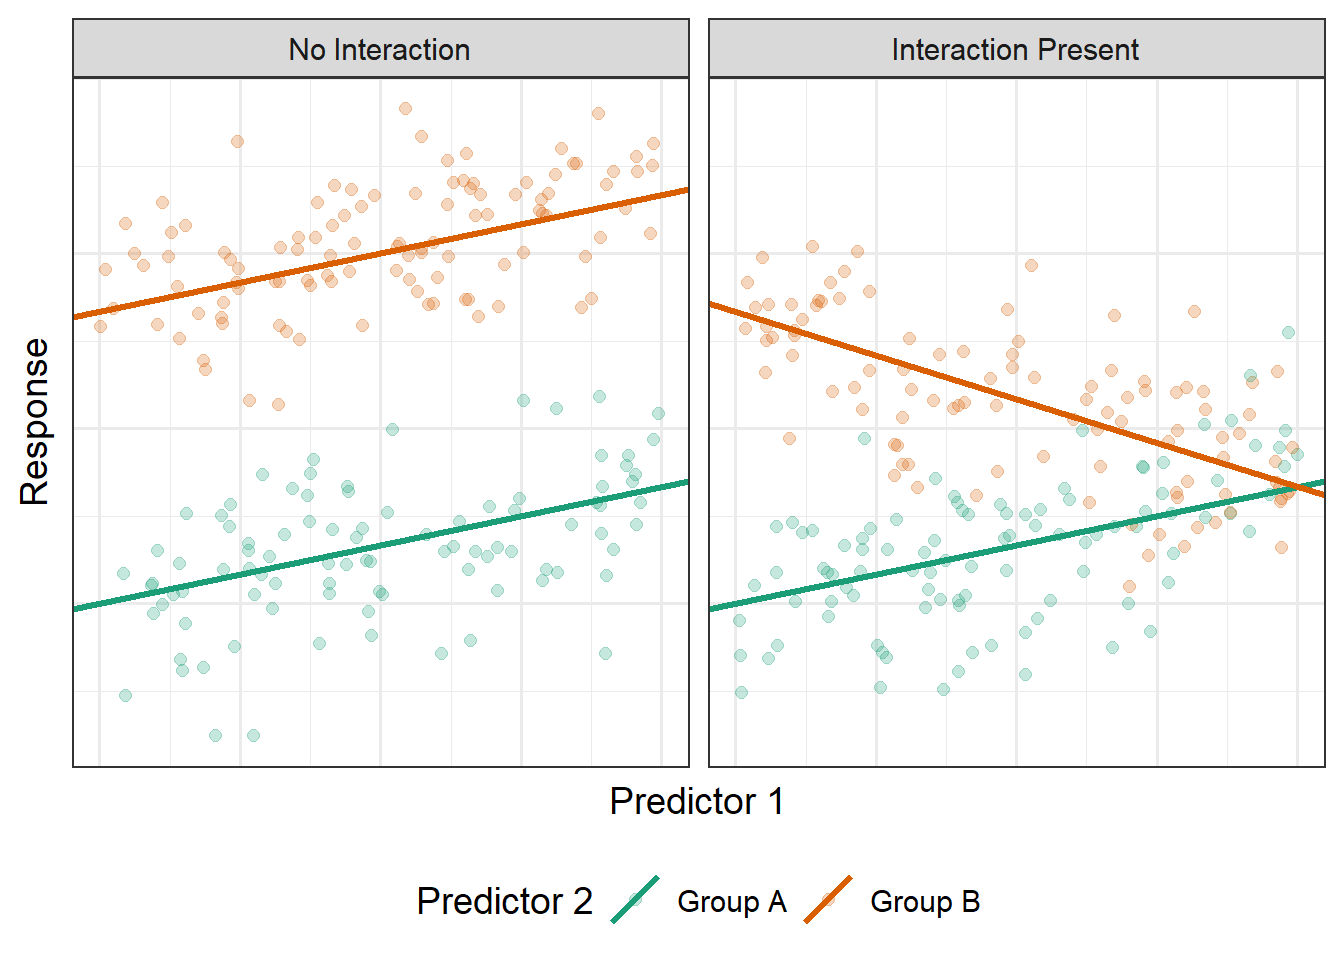
\includegraphics[width=0.8\textwidth]{./Images/glm-interactions-interactions-1} 

}

\caption{Illustration of the interaction of a quantitative and qualitative predictor on a response.}\label{fig:glm-interactions-interactions}
\end{figure}

Consider the following model:

\[(\text{Response})_i = \beta_0 + \beta_1 (\text{Predictor 1})_i + \beta_2 (\text{Group B})_i + \beta_3 (\text{Predictor 1})_i (\text{Group B})_i + \varepsilon_i.\]

We have added a third variable to the model that is the product of the first predictor and the group indicator. Let's examine the structure that is provided here. Suppose we are interested in examining the mean response for subjects in Group A; the value of \texttt{Group\ B} is 0 for these subjects, leading to

\[E\left[\text{Response} \mid \text{Predictor 1, Group A}\right] = \beta_0 + \beta_1 (\text{Predictor 1}).\]

For subjects in Group B, the value of \texttt{Group\ B} is 1, leading to the mean response

\[E\left[\text{Response} \mid \text{Predictor 2, Group B}\right] = \left(\beta_0 + \beta_2\right) + \left(\beta_1 + \beta_3\right) (\text{Predictor 1}).\]

This allows both the intercept and the slope to differ between the two groups. That is, it allows not only a ``bump'' for being in Group B to the mean response, but it also allows the effect of the first predictor to differ for the two groups.

\begin{rmdkeyidea}
In order to capture complex modeling structures, we embed those structures in a large model as opposed to fitting several smaller models in different subgroups of the population.
\end{rmdkeyidea}

\begin{definition}[Subgroup Analysis]

Refers to repeating a specified analysis (e.g., regression model) within various levels of a categorical predictor.

\begin{itemize}
\tightlist
\item
  This will appropriately estimate the effect modification.
\item
  It results in a loss of information because \emph{all parameters} are forced to vary across the subgroups.
\end{itemize}

\end{definition}

The predictor we added to our model (the product of two other predictors) is known as an interaction term.

\begin{definition}[Interaction]

An interaction term allows the effect of a predictor on the response to depend on the value of a second predictor (capturing an effect modification).

\begin{itemize}
\tightlist
\item
  This is created by adding the product of the two predictors under consideration to the model.
\end{itemize}

\end{definition}

While we have illustrated the use of interaction terms using a quantitative and categorical predictor, but interactions can be used with any type of predictors. Similarly, while we have illustrated the use of interaction terms in a linear model, this is a general modeling technique that can be extended to other forms of regression models.

\hypertarget{glm-linear-hypotheses}{%
\chapter{General Linear Hypothesis Test}\label{glm-linear-hypotheses}}

We previously discussed a model for the sampling distribution of the parameter estimates that allows for making inference on individual parameters; however, we do not yet have a way of testing more complex hypotheses. For example, testing whether the response is associated a categorical predictor involves determining if there is evidence that any of the coefficients associated with the indicator variables differs from zero. Such simultaneous tests fall under the General Linear Hypothesis framework.

While we write hypotheses as statements about parameters, we could also view them as comparisons of alternative models for the response.

\begin{rmdkeyidea}
Hypothesis testing is a way of determining if a simpler model (null hypothesis) is sufficient for explaining the variability in the response or if a more complex model (alternative hypothesis) is necessary. The simpler model is the result of placing \emph{constraints} on the complex model. Statistical significance is evidence that a more complex model is needed to capture the observed variability.
\end{rmdkeyidea}

The vast majority of scientific questions can be framed as a hypothesis which places a constraint on a more complex model for the data generating process. These constraints can in turn often be written as a linear combination of the parameters.

\begin{rmdtip}
For those less familiar with matrix algebra, a linear combination is simply the product of two vectors, and a series of linear combinations is the product of a matrix and a vector. Let \(\mathbf{K}\) be a 2-by-3 matrix defined as

\[\mathbf{K} = \begin{pmatrix} 
   K_{1,1} & K_{1,2} & K_{1,3} \\
   K_{2,1} & K_{2,2} & K_{2,3} \end{pmatrix}.\]

Let \(\boldsymbol{\beta}\) be a column vector of length 3 defined as

\[\boldsymbol{\beta} = \begin{pmatrix}
   \beta_1 \\
   \beta_2 \\
   \beta_3 \end{pmatrix}.\]

The product \(\mathbf{K} \boldsymbol{\beta}\) is defined as

\[\mathbf{K}\boldsymbol{\beta} = \begin{pmatrix}
   K_{1,1} \beta_1 + K_{1,2} \beta_2 + K_{1,3} \beta_3 \\
   K_{2,1} \beta_1 + K_{2,2} \beta_2 + K_{2,3} \beta_3 \end{pmatrix}\]

which is a vector of length 2. Each element in \(\mathbf{K}\boldsymbol{\beta}\) is a linear combination of the elements of \(\boldsymbol{\beta}\).
\end{rmdtip}

\begin{definition}[General Linear Hypothesis]

The general linear hypothesis refers to testing

\[H_0: \mathbf{K}\boldsymbol{\beta} = \mathbf{m} \qquad \text{vs.} \qquad H_1: \mathbf{K}\boldsymbol{\beta} \neq \mathbf{m}\]

where

\begin{itemize}
\tightlist
\item
  \(\boldsymbol{\beta}\) is the \((p+1)\)-length vector of the parameters (includes the intercept),
\item
  \(\mathbf{K}\) is an \(r\)-by-\((p+1)\) matrix that specifies the linear combinations defining the hypothesis of interest, and
\item
  \(\mathbf{m}\) is a vector of length \(r\) specifying the null values, the value of each linear combination under the null hypothesis (often a vector of 0's).
\end{itemize}

\end{definition}

Before discussing inference for this hypothesis, we discuss the most common use of this framework. Consider the following linear model:

\[(\text{Response})_i = \beta_0 + \beta_1 (\text{Predictor 1})_i + \beta_2 (\text{Predictor 2})_i + \varepsilon_i.\]

Suppose we are interested in testing the following hypotheses:

\[H_0: \beta_1 = \beta_2 = 0 \qquad \text{vs.} \qquad H_1: \text{At least one } \beta_j \text{ not equal to 0}.\]

To express this in the general linear hypothesis framework, we must identify the matrix \(\mathbf{K}\) and the vector \(\mathbf{m}\). Note that for this example

\[\boldsymbol{\beta} = \begin{pmatrix} 
\beta_0 \\
\beta_1 \\
\beta_2 \end{pmatrix}.\]

There are actually several choices for \(\mathbf{K}\), but we select the most straight-forward:

\[\mathbf{K} = \begin{pmatrix}
0 & 1 & 0 \\
0 & 0 & 1 \end{pmatrix} \qquad \text{with} \qquad \mathbf{m} = \begin{pmatrix}
0 \\ 0 \end{pmatrix}.\]

That is, the null hypothesis above can be stated as

\[\begin{pmatrix} 0 & 1 & 0 \\ 0 & 0 & 1 \end{pmatrix} \boldsymbol{\beta} = \begin{pmatrix} 0 \\ 0 \end{pmatrix}.\]

\begin{rmdtip}
When developing the matrix \(\mathbf{K}\), the number of rows corresponds to the number of equal signs in the null hypothesis.
\end{rmdtip}

The general linear hypothesis allows us to say something about multiple parameters (or combinations of parameters) \emph{simultaneously}. Each linear combination is not a separate hypothesis; together, they form a ``joint'' hypothesis. That is, we should think of each linear combination defined by the rows of \(\mathbf{K}\) as ``and'' statements; we want every statement to be true at the same time. The framework is extremely flexible and can be used across several types of statistical models. It allows us to write the hypotheses compactly, mostly for communicating them to a computer. However, the framework alone does not produce p-values for such tests. In order to obtain a p-value, we need a model for the null distribution. As the hypothesis involve many parameters, we cannot (and should not) test each statement separately.

To fully understand the previous statement requires a background in statistical theory. We hand-wave this by saying that our parameter estimates are related. This is somewhat intuitive. Imagine trying to develop a line that runs through a cloud of points (see Figure \ref{fig:glm-linear-hypotheses-line}); if we constrain the line to go through the ``middle'' of the data (the point represented by the average of the predictor and the average of the response), then changing the slope of the line will necessarily change the intercept of the line. We extend this intuition by claiming that the estimate of one coefficient is related to the estimate of the parameters in a model.

\begin{figure}

{\centering 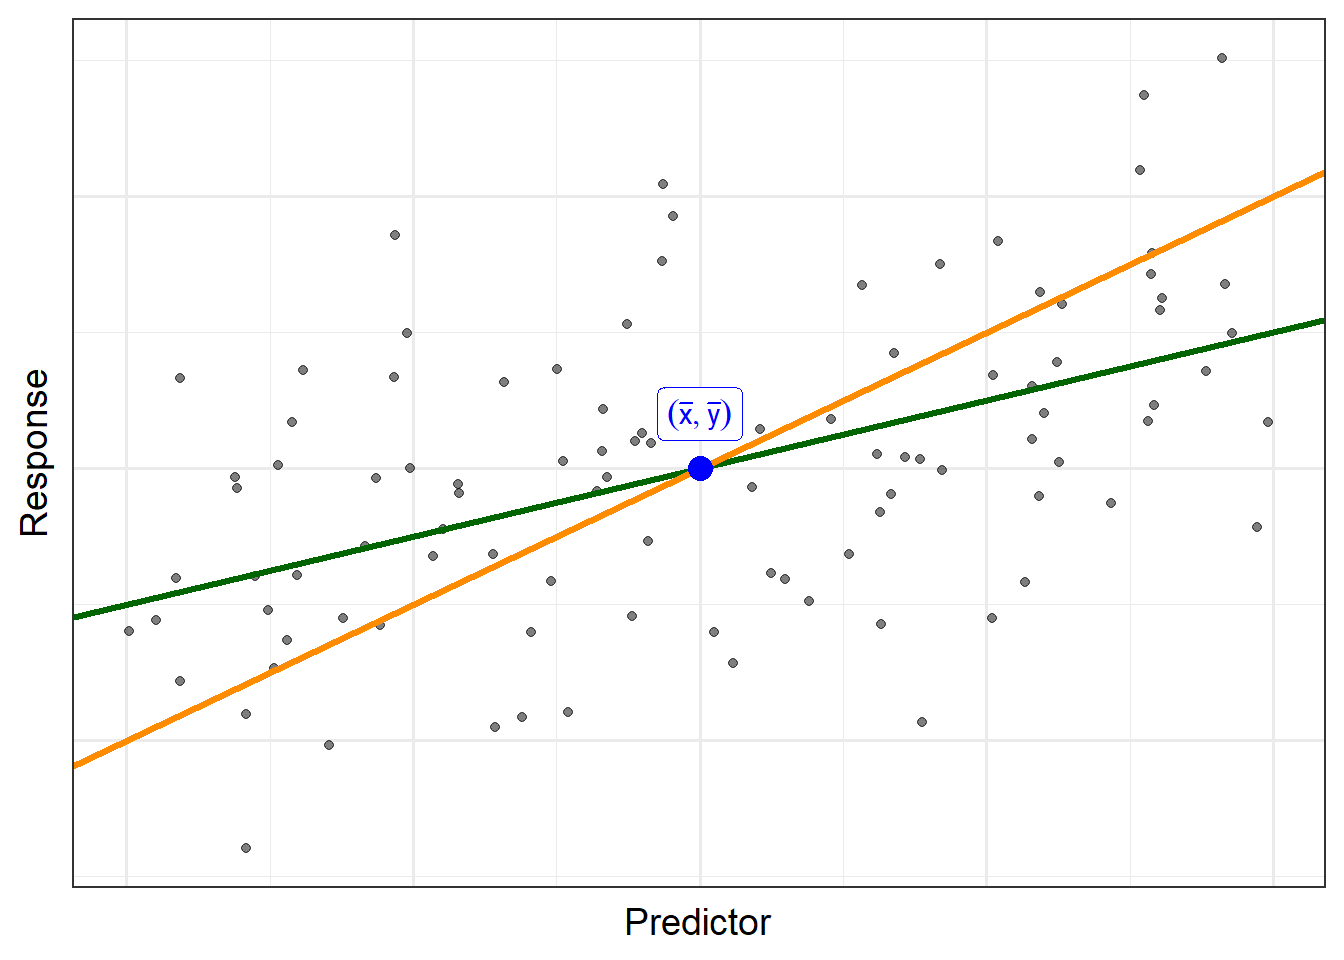
\includegraphics[width=0.8\textwidth]{./Images/glm-linear-hypotheses-line-1} 

}

\caption{Illustration of the relationship between parameter estimates.}\label{fig:glm-linear-hypotheses-line}
\end{figure}

We know that the standard error is a measure of the variability in an estimate; we could just as easily use their variance (the square of the standard error). A convenient measure of the relationship between the estimates is known as their covariance. We store this information in the variance-covariance matrix.

\begin{definition}[Variance-Covariance Matrix]

Let \(\boldsymbol{\beta}\) represent the \((p+1)\)-length vector of the parameters and \(\widehat{\boldsymbol{\beta}}\) represent the \((p+1)\) vector of the parameter \emph{estimates}. The variance-covariance matrix of the parameter estimates is the \((p+1)\)-by-\((p+1)\) matrix \(\boldsymbol{\Sigma}\) where

\begin{itemize}
\tightlist
\item
  the \(j\)-th diagonal element contains \(Var\left(\widehat{\beta}_j\right)\), and
\item
  the \((i,j)\)-th element contains the covariance between \(\widehat{\beta}_i\) and \(\widehat{\beta}_j\).
\end{itemize}

\end{definition}

The variance-covariance matrix is an extremely important concept in statistical theory; here, we simply note that it is contains information on the structure of how the estimates are related to one another. We further note that this is computed automatically in most software. We are now in a place to discuss inference for the general linear hypothesis.

\begin{definition}[Model for the Null Distribution with the General Linear Hypothesis]
Let \(\widehat{\boldsymbol{\beta}}\) be the \((p+1)\) vector of estimates for the parameter vector \(\boldsymbol{\beta}\), and let the estimates have variance-covariance matrix \(\boldsymbol{\Sigma}\). Assuming the null hypothesis

\[H_0: \mathbf{K} \boldsymbol{\beta} = \mathbf{m}\]

is true, under the conditions of the classical regression model

\[(1/r) \left(\mathbf{K}\widehat{\boldsymbol{\beta}} - \mathbf{m}\right)^\top \left(\mathbf{K}\widehat{\boldsymbol{\Sigma}}\mathbf{K}^\top\right)^{-1} \left(\mathbf{K}\widehat{\boldsymbol{\beta}} - \mathbf{m}\right) \sim F_{r, n-p-1}\]
\end{definition}

Again, the specifics of the above result are not as important as understanding there exists a standardized statistic for which the null distribution can be modeled explicitly, as an F-distribution with \(r\) numerator degrees of freedom and \(n-p-1\) denominator degrees of freedom. While the denominator degrees of freedom are associated with the scaling term for the residual variance estimate, the numerator degrees of freedom are associated with the complexity of the hypothesis (the number of rows of \(\mathbf{K}\)).

While the theory that provides the above results holds only for the linear model under the classical regression model, the approach we have outlined here will allow us to provide general results which are applicable under many types of regression models.

\hypertarget{glm-large-sample-theory}{%
\chapter{Large Sample Theory}\label{glm-large-sample-theory}}

The classical regression model (Definition \ref{def:defn-classical-regression}) imposes several conditions on the distribution of the error term. These conditions define the model for the sampling distributions needed to make inference on the parameters. However, these conditions are not always reasonable. Fortunately, many of the conditions can be relaxed. In this chapter, we consider relaxing Normality condition.

\hypertarget{two-types-of-models}{%
\section{Two Types of Models}\label{two-types-of-models}}

In general, there are two general types of models for a data generating process: parametric and semiparametric models.

\begin{definition}[Parametric Model]
A parametric model assumes we can \emph{fully} characterize the distribution of the response given the predictors.
\end{definition}

\begin{definition}[Semiparametric Model]
A semiparametric model specifies some components of the underlying distribution (e.g., mean and variance) of the response, but does not fully characterize it.
\end{definition}

\begin{rmdtip}
Technically, semiparametric models are a subset nonparametric models --- those which do not fully characterize the distribution of the response. However, semiparametric models are often considered a distinct type of model because they have elements of both parametric models (there are some parameters to be estimated) and nonparametric models (completely data-driven).
\end{rmdtip}

Parametric models make strong assumptions, but often make the analysis straight-forward as we are able to make use of a large class of results from statistical theory. This is very useful when we have a small sample size in particular. Nonparametric models extremely flexible, but they require substantially large sample sizes. Semiparametric models, in turn, often find a the ``sweet spot.'' They require larger samples than a parametric model, but not as large as a nonparametric model. Further, the scientific question of interest is still represented through statements about parameters in the model, linking the interpretations more directly with practical application.

The alternate characterization of the classical regression model (Definition \ref{def:defn-alternate-characterization}) reveals that the classical regression model is a parametric model. It completely characterizes the distribution of the response:

\[(\text{Response})_i \mid (\text{Predictors 1 through } p)_i \stackrel{\text{Ind}}{\sim}N\left(\beta_0 + \sum\limits_{j=1}^{p} \beta_j (\text{Predictor } j)_i, \sigma^2\right).\]

This is a very strong assumption. Further, often the questions posed by the researchers do not concern the form of the distribution of the response but only some aspect of the distribution. For example, the hypotheses we have considered thus far in the text surround the parameters of the mean model; that is, we have concerned ourselves only with questions regarding the \emph{mean} response. Since most scientific questions focus on the mean response, we are led to positing a semiparametric linear model.

\begin{definition}[Semiparametric Linear Model]
Suppose we no longer require that the error terms follow a Normal distribution; however, we do continue to impose the remaining conditions of the classical regression model. Then, our model could be written as

\[
\begin{aligned}
  E\left[(\text{Response})_i \mid (\text{Predictors 1 through } p)_i\right]
    &= \beta_0 + \sum\limits_{j=1}^{p} \beta_j (\text{Predictor } j)_i \\
  Var\left[(\text{Response})_i \mid (\text{Predictors 1 through } p)_i\right]
    &= \sigma^2
\end{aligned}
\]

where the responses are independent of one another given the predictors.
\end{definition}

Notice that this version of the model only specifies aspects of the response distribution; it specifies that the mean is a linear combination of the predictors, and it specifies that the variance is constant. However, it does not specify the functional form of the distribution.

\hypertarget{large-sample-results}{%
\section{Large Sample Results}\label{large-sample-results}}

The primary benefit of a parametric model is that often the distributional assumption trickles through the analysis and allows us to exactly specify the model for the sampling distribution. When we move to a semi-parametric model, we need additional tools to allow us to model the sampling distribution. One such tool is large-sample theory.

\begin{definition}[Large Sample Theory]
When a model for the sampling distribution (or null distribution) of an estimate (or standardized statistic) is known as the sample size becomes infinitely large. That is, as the sample size approaches infinity, the sampling distribution (or null distribution) can be easily modeled using a known probability distribution.
\end{definition}

Perhaps the most well-known example of large-sample theory is the Central Limit Theorem encountered in introductory statistics.

\begin{definition}[Central Limit Theorem]
Let \(Y_1, Y_2, \dotsc, Y_n\) be independent and identically distributed random variables with mean \(\mu\) and variance \(\sigma^2\). Then, as \(n\) approaches infinity

\[\frac{\sqrt{n}\left(\bar{Y} - \mu\right)}{\sigma} \sim N(0, 1).\]
\end{definition}

Putting this in the language of this text, this states that as the sample size gets large, the standardized distance between the average response observed and the true average response can be modeled using a Normal distribution with mean 0 and variance 1. Notice that the theorem does not specify the distribution of the response \(Y\); it only specifies the mean and variance. That is, we began with a semiparametric model and obtained a model for the sampling distribution. We exchanged the condition that the response follow a Normal distribution for the condition that ``the sample size be sufficiently large'' that the model is reasonable.

It turns out that similar results can be derived for the semiparametric linear model. That is, in large samples, we can approximate the sampling distribution of our estimates and the null distribution of our standardized statistics.

\begin{definition}[Large Sample Model for the Sampling Distribution of Least Squares Estimates]
Suppose the classical regression conditions hold, with the exception of the errors following a Normal distribution. As the sample size gets large, we have that

\[\frac{\widehat{\beta}_j - \beta_j}{\sqrt{Var\left(\widehat{\beta}_j\right)}} \sim N(0, 1)\]

for all \(j = 0, 1, \dotsc, p\). Further, under the null hypothesis

\[H_0: \mathbf{K}\boldsymbol{\beta} = \mathbf{m}\]

we have

\[\left(\mathbf{K}\widehat{\boldsymbol{\beta}} - \mathbf{m}\right)^\top \left(\mathbf{K}\widehat{\boldsymbol{\Sigma}}\mathbf{K}^\top\right)^{-1} \left(\mathbf{K}\widehat{\boldsymbol{\beta}} - \mathbf{m}\right) \sim \chi^2_r.\]
\end{definition}

Notice that our statistics and standardized statistic have a similar form as before; the difference is the probability model being used. In place of a t-distribution, we have a Normal distribution. In place of the F-distribution, we have a Chi-Square distribution. This result allows us to perform inference even if we are unwilling to assume the errors follow a Normal distribution.

It is natural to ask how large of a sample size is required for these models to be reasonable; there is no simple answer. Empirical studies suggest that in practice, if we have at least 30 degrees of freedom for estimating the error term, these results are often reasonable.

\begin{rmdtip}
Not all software implements methods for relying on these large-sample results. However, as the sample size gets large, it turns out that classical inference and the large-sample results coincide. That is, the confidence intervals and p-values we would compute using the large-sample models and those obtained assuming the classical regression model are nearly identical. Therefore, in practice, when the sample size is large, we can rely on the default output even if we are unwilling to assume the errors follow a Normal distribution.
\end{rmdtip}

\hypertarget{residual-bootstrap}{%
\section{Residual Bootstrap}\label{residual-bootstrap}}

An alternative to large-sample theory is building an empirical model for the sampling distribution (or null distribution) when working with a semiparametric model known as bootstrapping.

\begin{definition}[Bootstrapping]
A process of resampling the data and estimating the parameters of interest in each resample to construct an empirical model of the sampling distribution.
\end{definition}

There are several bootstrapping algorithms; the most foundational for regression modeling is the residual bootstrap.

\begin{definition}[Residual Bootstrap]
Suppose we observe a sample of size \(n\) and use it to fit the linear model

\[(\text{Response})_i = \beta_0 + \sum_{j=1}^{p} \beta_j (\text{Predictor } j)_i + \varepsilon_i\]

and obtain the least squares estimates \(\widehat{\boldsymbol{\beta}}\). The residual bootstrap proceeds along the following algorithm:

\begin{enumerate}
\def\labelenumi{\arabic{enumi}.}
\tightlist
\item
  Compute the residuals
  \[(\text{Residuals})_i = (\text{Response})_i - (\text{Predicted Response})_i\]
\item
  Take a random sample of size \(n\) (with replacement) of the residuals; call the values \(e_1^*, \dotsc, e_n^*\).
\item
  Form ``new'' responses \(y_1^*, \dotsc, y_n^*\) according to
  \[y_i^* = \widehat{\beta}_0 + \sum_{j=1}^{p} \widehat{\beta}_j (\text{Predictor } j)_i + e_i^*.\]
\item
  Obtain the least squares estimates \(\widehat{\boldsymbol{\alpha}}\) by finding the values of \(\boldsymbol{\alpha}\) which minimize
  \[\sum_{i=1}^{n} \left(y_i^* - \alpha_0 - \sum_{j=1}^{p} \alpha_j (\text{Predictor } j)_i\right)^2.\]
\item
  Repeat steps 2-4 \(m\) times.
\end{enumerate}

We often take \(m\) to be large (at least 1000). After each pass through the algorithm, we retain the least squares estimates from the resample. The distribution of the estimates across these resamples is a good empirical model for the sampling distribution of the original least squares estimates.
\end{definition}

While the residual bootstrap is the foundation of many similar algorithms, it is perhaps not as easy to understand as the case-resampling bootstrap.

\begin{definition}[Case Resampling Bootstrap]
Suppose we observe a sample of size \(n\) and use it to fit the linear model

\[(\text{Response})_i = \beta_0 + \sum_{j=1}^{p} \beta_j (\text{Predictor } j)_i + \varepsilon_i\]

and obtain the least squares estimates \(\widehat{\boldsymbol{\beta}}\). The residual bootstrap proceeds along the following algorithm:

\begin{enumerate}
\def\labelenumi{\arabic{enumi}.}
\tightlist
\item
  Take a random sample of size \(n\) (with replacement) of the raw data (keeping all variables from the same observation together).
\item
  Obtain the least squares estimates \(\widehat{\boldsymbol{\alpha}}\) by finding the values of \(\boldsymbol{\alpha}\) which minimize
  \[\sum_{i=1}^{n} \left((\text{Response})_i^* - \alpha_0 - \sum_{j=1}^{p} \alpha_j (\text{Predictor } j)_i^*\right)^2.\]
\item
  Repeat steps 1-2 \(m\) times.
\end{enumerate}

We often take \(m\) to be large (at least 1000). After each pass through the algorithm, we retain the least squares estimates from the resample. The distribution of the estimates across these resamples is a good empirical model for the sampling distribution of the original least squares estimates.
\end{definition}

The case-resampling bootstrap procedure is easier to visualize as we are resampling the data observed. The residual bootstrap resamples the residuals; this mimics generating new observations by ``jittering'' points away from the estimated regression line. In both algorithms, the same model is refit on the resample producing new estimates. The collection of these estimates across the \(m\) resamples is our model for the sampling distribution (which could be visualized using a histogram, for example).

The theoretical underpinnings of bootstrapping (and how it is implemented efficiently in software) is beyond the scope of this text. What we emphasize is that through this process, we construct a model for the sampling distribution of the estimates, which allows us to compute confidence intervals. Further, the residual bootstrap requires the same conditions as the classical regression model, with the exception of requiring the errors to follow a Normal distribution. That is, it has the same conditions as we stated for our semiparametric regression model above.

\begin{rmdtip}
Technically, the case-resampling bootstrap and the residual bootstrap require different conditions, with the case-resampling bootstrap being less restrictive. However, at this point, we do not make a distinction between which bootstrap algorithm is utilized.
\end{rmdtip}

Bootstrapping is more computationally burdensome than large-sample theory, but it allows us to build valid confidence intervals even in smaller sample sizes.

\begin{rmdtip}
While theoretically, bootstrapping can be used with any sample size, it has been shown to yield more reliable results in large samples.
\end{rmdtip}

\hypertarget{big-picture}{%
\section{Big Picture}\label{big-picture}}

We have discussed two alternatives to using inference results from the classical regression model when we are unwilling to assume the errors follow a Normal distribution. Again, these results were discussed in the context of the linear model, but they illustrate a concept that holds across many types of regression models --- there are essentially three ways to build a model for the sampling distribution. In order to perform inference on a set of parameters, we need a model for the sampling distribution (or null distribution).

\begin{rmdkeyidea}
There are three options for modeling the sampling distribution:

\begin{enumerate}
\def\labelenumi{\arabic{enumi}.}
\tightlist
\item
  Exact Probability Theory: often the result of assuming a parametric model, the sampling distribution of the resulting parameter estimates is known.
\item
  Large-Sample Theory: often employed in semiparametric models, the sampling distribution of the resulting parameter estimates can be approximated as the sample size gets large.
\item
  Empirical: often employed in semiparametric models, the sampling distribution of the resulting parameter estimates is modeled through resampling.
\end{enumerate}
\end{rmdkeyidea}

We will see as we move throughout the text that we often move between these various approaches. However, which approach we take is governed by the conditions we are willing to impose on the data generating process.

We end with a common question: if we are able to model the sampling distribution without fewer conditions, why would we not always take that approach? The closer the conditions are to the true data generating process, the more powerful our analysis; that is, if the errors are truly Normally distributed, then imposing that condition will make it more likely for us to find a signal that really exists. So, we battle the tension of a more powerful analysis with one which is more flexible. We adhere to the belief that we should choose the approach which is most consistent with the available data.

\hypertarget{glm-splines}{%
\chapter{Modeling Curvature}\label{glm-splines}}

In addition to conditions on the error term, the classical regression model (Definition \ref{def:defn-classical-regression}) requires that the predictors enter the model linearly. It is often the case, however, that the relationship between the response and a predictor is not linear, even after accounting for other predictors. Ignoring this curvature, essentially leaving the deterministic portion of the model incorrectly specified, can result in incorrect conclusions. Fortunately, the linear model framework is flexible enough to model curvature. This may seem to be a contradiction, but it relies on the definition of what it means for a model to be linear.

\begin{definition}[Linear Model]
A model is said to be linear if it is linear in the \emph{parameters}. That is, the linearity does not refer to the form of the predictors but that the deterministic portion of the model is specified as a linear combination of the parameters for each observation.
\end{definition}

The beauty of this understanding of linearity is that it allows us to capture curvature, provided that we can represent that curvature through the addition of predictors. As a simple example, suppose we have a response that is parabolically related to a predictor (Figure \ref{fig:glm-splines-parabola}).

\begin{figure}

{\centering 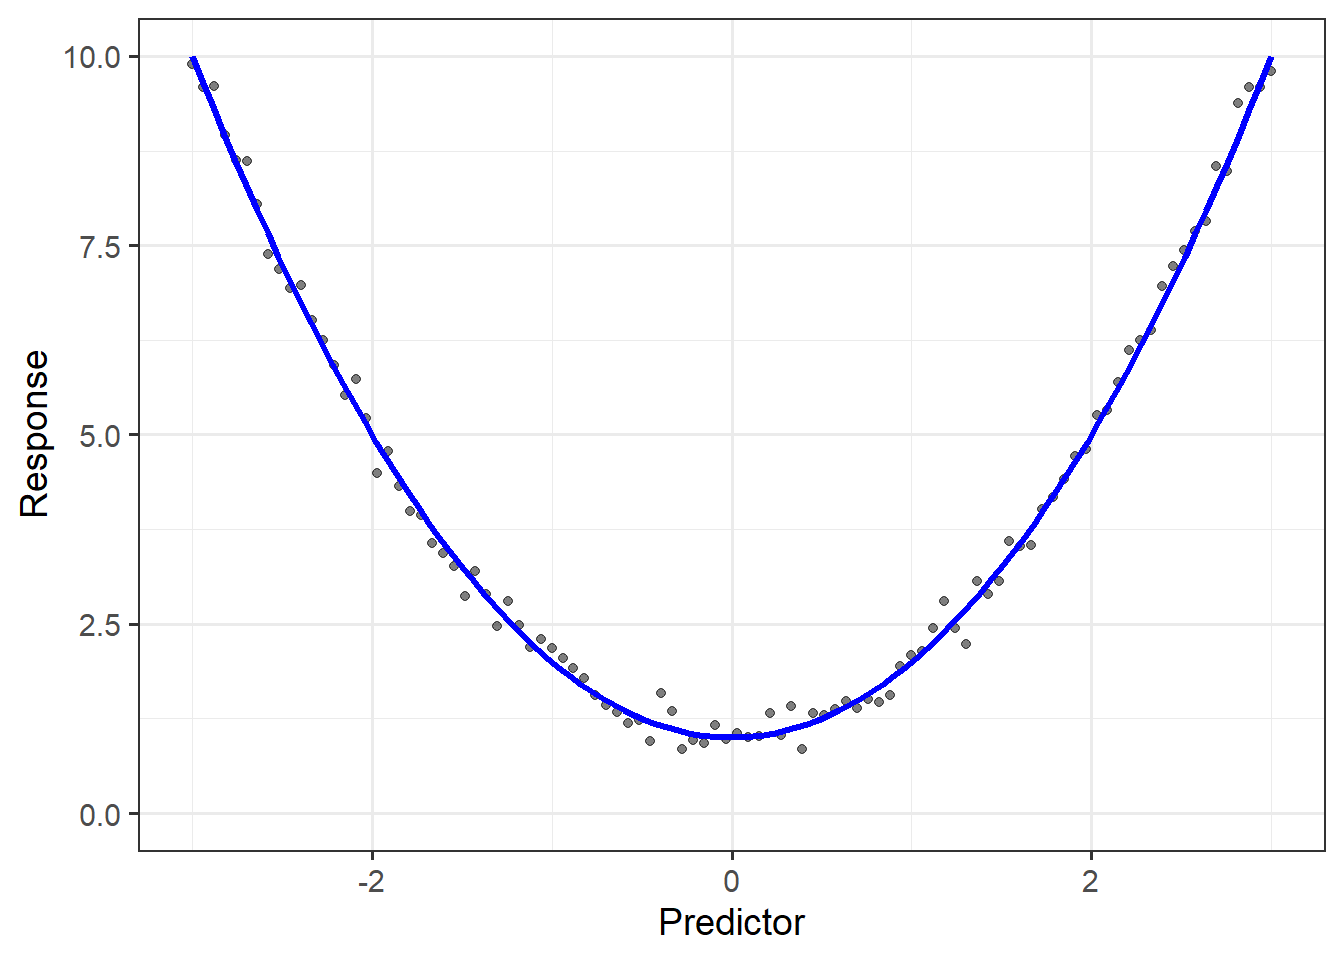
\includegraphics[width=0.8\textwidth]{./Images/glm-splines-parabola-1} 

}

\caption{Illustration of a parabolic relationship between a response and a predictor.}\label{fig:glm-splines-parabola}
\end{figure}

This linear model could be represented as

\[(\text{Response})_i = \beta_0 + \beta_1 (\text{Predictor})_i^2 + \varepsilon_i.\]

The mean response will clearly generate curvature, but the deterministic portion is linear in the parameters; let \(\mathbf{x}_i\) represent the vector of all predictors for the \(i\)-th observation, including the intercept. In this case we have

\[\mathbf{x}_i = \begin{pmatrix} 1 \\ (\text{Predictor})_i \end{pmatrix}.\]

Then, we can write the above model as

\[(\text{Response})_i = \mathbf{x}_i^\top \boldsymbol{\beta}+ \varepsilon_i\]

where we have that the deterministic portion is the product of two vectors; being able to express the model in this form is the definition of a linear model.

\begin{rmdtip}
For those not as comfortable with matrix algebra, essentially, the model will be linear as long as we can express it in the form

\[(\text{Response})_i = \beta_0 + \sum_{j=1}^{p} \beta_j (\text{Something not involving parameters})_i + \varepsilon_i\]

even if some of the components involve nonlinear transformations of variables in our data set.
\end{rmdtip}

Due to this flexibility, we are interested in investigating transformations of the predictors to add to the model that would capture curvature. In the above example, we knew the form of the curvature we wanted to model (a parabola shifted up from the origin). In practice, we often will not know the form of the curvature, just that it exists (from the plots of the residuals against the predictor). And, that curvature may not be modeled well with a high-degree polynomial (or would require a polynomial of such a high degree it would not be practical). In such cases, we use the idea of a spline.

\begin{definition}[Spline]
A spline is a piecewise polynomial used in fitting curves. A \emph{linear} spline is comprised only of linear pieces. The points that define the piecewise components are called \emph{knot points}; these are where the functional form is allowed to change.
\end{definition}

A linear spline is perfect for capturing relationships which appear to be linear over regions, but for which the relationship is different in each of those regions. For example, a ``V'' relationship would suggest that as the predictor increases, the response tends to decrease in the first region; however, in the second region, as the predictor increases, the response tends to increase as well. A linear spline can be placed into the linear model framework.

\begin{definition}[Formula for Linear Spline]
A response can be related to a predictor using a linear spline with \(k\) knot points, call them \(t_1, t_2, \dotsc, t_k\) using the following formula:

\[(\text{Response})_i = \beta_0 + \beta_1 (\text{Predictor})_i + \sum_{j=1}^{k} \beta_{j+1} \left((\text{Predictor})_i - t_j\right)_{+} + \varepsilon_i\]

where \(u_{+}\) takes the value \(u\) when \(u > 0\) and takes the value 0 otherwise. Capturing curvature using a linear spline with \(k\) knot points requires \(k\) additional terms.
\end{definition}

Figure \ref{fig:glm-splines-linear-spline} illustrates a linear spline with two knot points.

\begin{figure}

{\centering 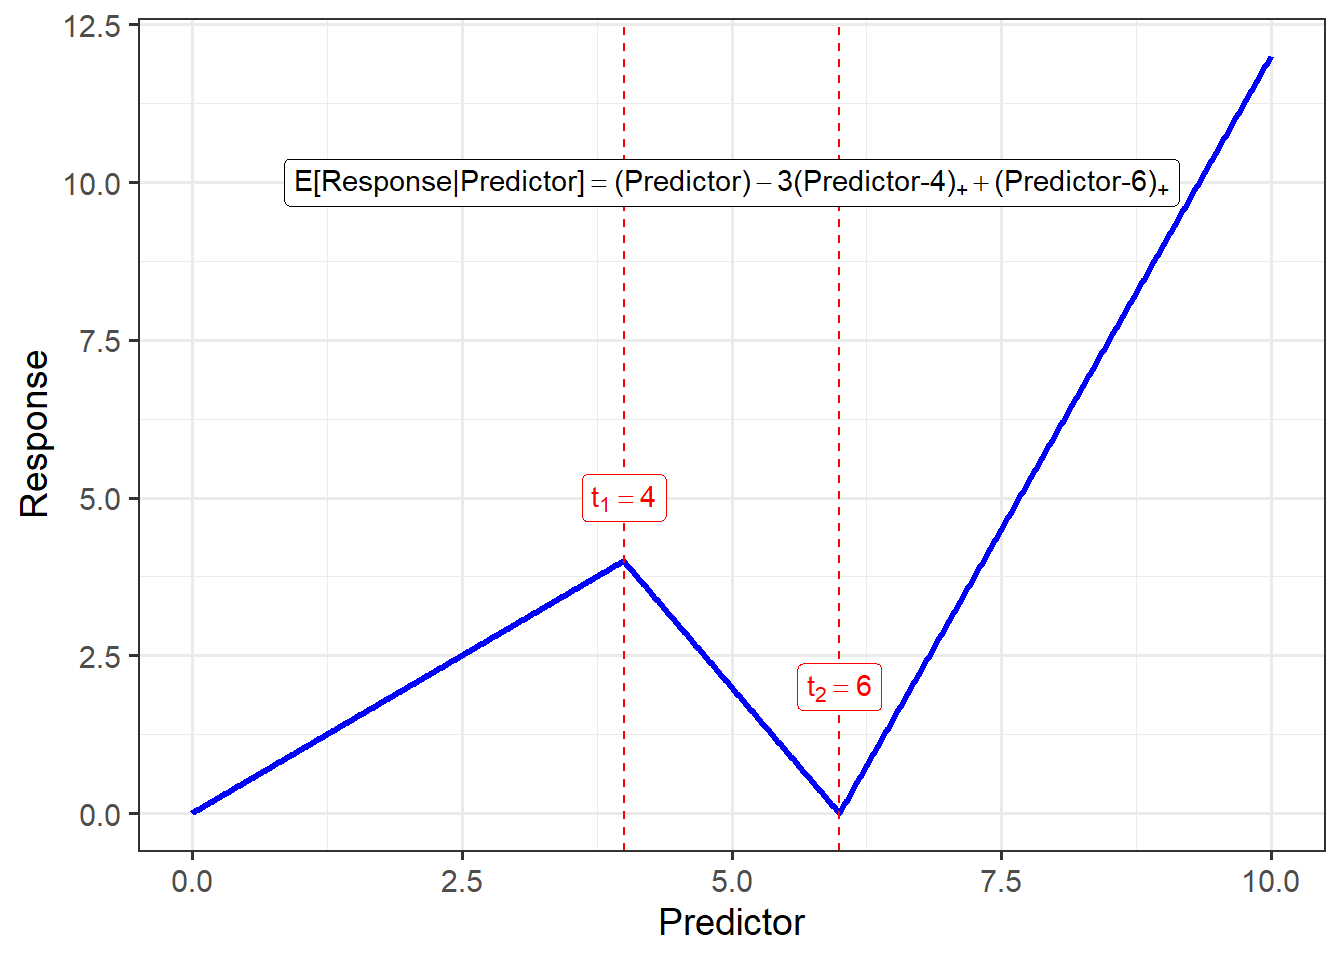
\includegraphics[width=0.8\textwidth]{./Images/glm-splines-linear-spline-1} 

}

\caption{Illustration of a linear spline with two knot points.}\label{fig:glm-splines-linear-spline}
\end{figure}

\begin{rmdtip}
In practice, the knot points for the linear spline are generally determined by the discipline expert based on some scientific reason why the relationship might change at that particular value.
\end{rmdtip}

While the above definition of the linear spline considers only a single predictor, we can add a spline to a model which has additional predictors. Further, once we have these additional elements in the model, we can actually perform a hypothesis test to determine if the additional complexity is needed. Considering the above definition of a linear spline, the hypothesis

\[H_0: \beta_2 = \beta_3 = \dotsc = \beta_{k+1} = 0\]

suggests that a linear relationship is sufficient for modeling the relationship between the response and the predictor.

There are plenty of forms of curvature which would not be captured by a linear spline. When we have a more complex relationship that needs to be modeled, we can use a restricted cubic spline.

\begin{definition}[Restricted Cubic Spline]
A restricted cubic spline is comprised of piecewise cubic polynomials for which the tails of the spline have been restricted to be linear.
\end{definition}

Restricted cubic splines (related to natural splines in the computational science community) are smooth at the knot points (meaning they have nice mathematical properties). Further, it has been shown empirically that restricted cubic splines are often flexible enough to approximate nearly any nonlinear relationship. Again, these are able to be embedded in the linear framework.

\begin{definition}[Formula for Restricted Cubic Spline]
A response can be related to a predictor using a restricted cubic spline with \(k\) knot points, call them \(t_1, t_2, \dotsc, t_k\) using the following formula:

\[(\text{Response})_i = \beta_0 + \beta_1 (\text{Predictor})_i + \sum_{j=1}^{k-2} \beta_{j+1} x_{j,i} + \varepsilon_i\]

where

\[
\begin{aligned}
  x_{j,i} &= \left((\text{Predictor})_i - t_j\right)^3_{+} - \frac{\left((\text{Predictor})_i - t_{k-1}\right)^3_{+} \left(t_k - t_j\right)}{t_k - t_{k-1}} \\
    &\qquad +\frac{\left((\text{Predictor})_i - t_k\right)^3_{+} \left(t_{k-1} - t_j\right)}{t_k - t_{k-1}}
\end{aligned}
\]

where \(u_{+}\) takes the value \(u\) when \(u > 0\) and takes the value 0 otherwise. Capturing curvature using a restricted cubic spline with \(k\) knot points requires \(k-2\) additional terms.

Empirical studies have shown that generally only \(k = 5\) knot points are needed, and these are set at the 5-th, 27.5-th, 50-th, 72.5-th, and 95-th percentiles. This ensures there is enough data in each region to appropriately capture the curvature.
\end{definition}

Similar to linear splines, we can add a restricted cubic spline for a variable to a model which has additional predictors. Further, once we have these additional elements in the model, we can actually perform a hypothesis test to determine if the additional complexity is needed. Considering the above definition of a restricted cubic spline, the hypothesis

\[H_0: \beta_2 = \beta_3 = \dotsc = \beta_{k-1} = 0\]

suggests that a linear relationship is sufficient for modeling the relationship between the response and the predictor. Figure \ref{fig:glm-splines-restricted-cubic-spline} illustrates a restricted cubic spline with five knot points. We point out that there is quite a bit of curvature here, and yet this is captured by a linear model!

\begin{figure}

{\centering 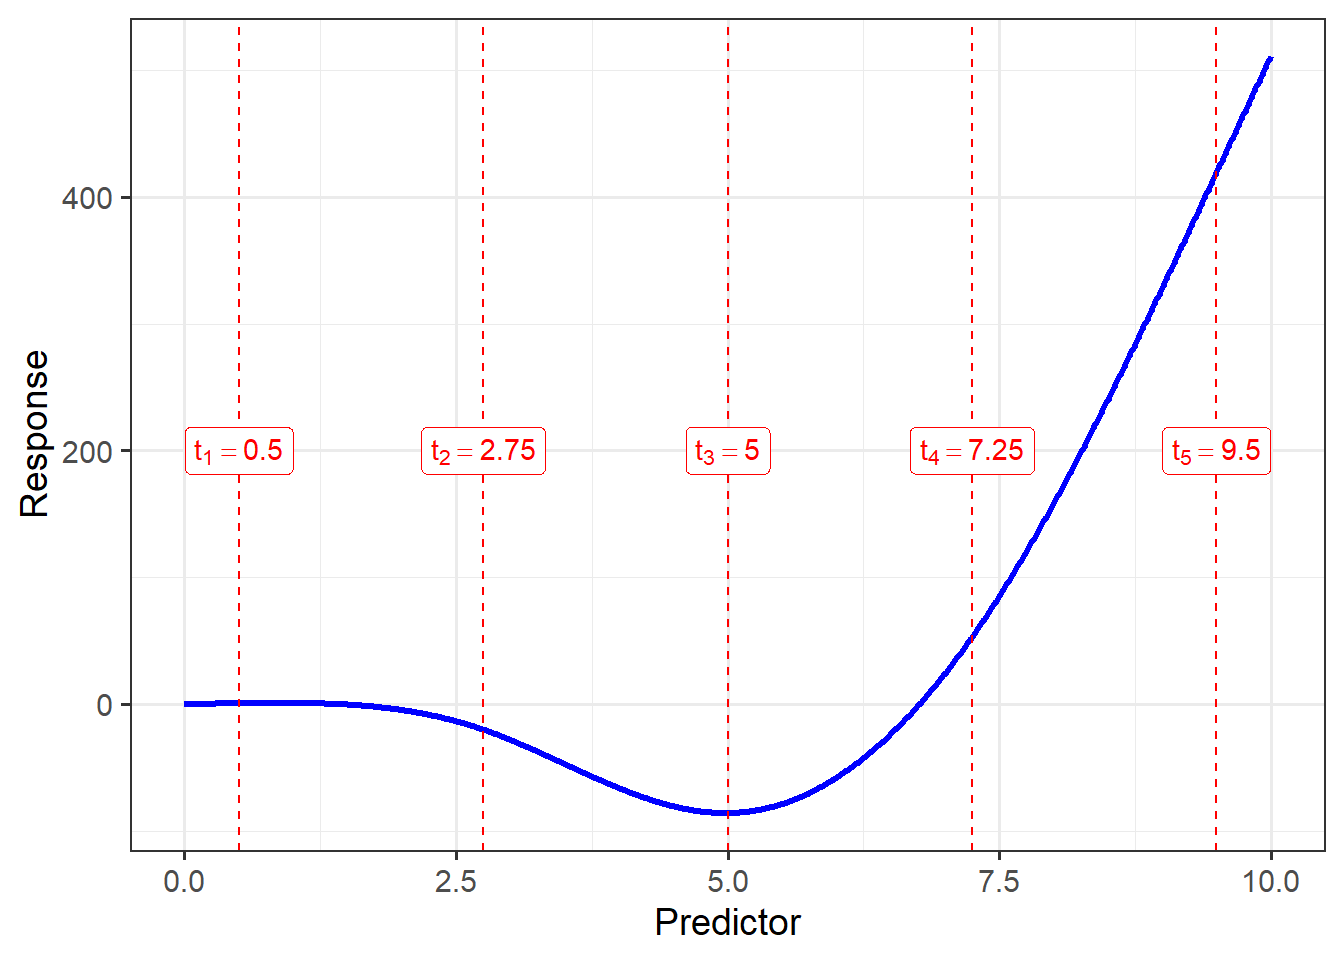
\includegraphics[width=0.8\textwidth]{./Images/glm-splines-restricted-cubic-spline-1} 

}

\caption{Illustration of a restricted cubic spline with five knot points.}\label{fig:glm-splines-restricted-cubic-spline}
\end{figure}

Both types of splines can be fit using standard software if we are willing to program the above formulas; however, statistical software often has a direct implementation. This is a benefit over nonparametric approaches which require more advanced computation implemented only in statistical software. Further, by placing this in a semiparametric framework, we are able to model complex curvature with smaller sample sizes.

Linear splines allow for very easy interpretation since the relationships are linear in each region. Restricted cubic splines, in contrast, have intractable interpretations but provide a lot of flexibility. In general, if the predictor which requires a spline is the primary variable of interest, we recommend trying a linear spline. If however, the predictor is just being adjusted for in the model, and the curvature is not of primary importance, using a restricted cubic spline with five knot points is sufficient.

\begin{rmdtip}
When a categorical predictor is modeled using a series of indicator variables, linearity cannot be violated for these components. Since there are only two levels for each indicator variable, a line \emph{must} be an appropriate relationship; therefore, violations of linearity and their subsequent adjustments are only considered for quantitative predictors.
\end{rmdtip}

As in the previous chapters of this unit, we introduced splines in the context of the linear model. However, they can be incorporated into a vast number of regression models.

\hypertarget{part-models-for-repeated-measures}{%
\part{Models for Repeated Measures}\label{part-models-for-repeated-measures}}

\hypertarget{rm-terminology}{%
\chapter{Terminology}\label{rm-terminology}}

When the same response is collected multiple times on a single subject, the assumption of independence is almost certainly violated. In order to obtain valid inference, the correlation introduced in the data should be appropriately modeled. Understanding these models can lead to more powerfully designed studies.

\hypertarget{importance-of-study-design}{%
\section{Importance of Study Design}\label{importance-of-study-design}}

Study design is too often separated from the statistical analysis that follows. However, in addition to informing the conclusions we draw regarding the data, the study design helps in choosing an appropriate analysis to address the question of interest. As an example, consider the following study reported in Vittinghoff et al. (\protect\hyperlink{ref-Vittinghoff2012}{2012}).

\begin{example}[Digestive Enzymes]
The ability of the bowels to properly absorb nutrients can be impacted by a lack of digestive enzymes. This presents as excess fat in the feces. Pancreatic enzyme supplements can be given to ameliorate the problem. A study was conducted comparing three forms of a particular enzyme supplement; these were compared to no supplement (placebo) as a control. Subjects were given the supplement to take for a specified length of time; then, the amount of fecal fat (g/day) present was recorded. The data is presented in Table \ref{tab:rm-enzyme-data-table}.

Interest is in determining if the amount of fecal fat produced, on average, differed for any of the treatments.
\end{example}

\begin{table}

\caption{\label{tab:rm-enzyme-data-table}Data from study comparing different forms of an enzyme supplement.}
\centering
\begin{tabular}[t]{lrrrrrr}
\toprule
Placebo & 44.5 & 33.0 & 19.1 & 9.4 & 71.3 & 51.2\\
Tablet & 7.3 & 21.0 & 5.0 & 4.6 & 23.3 & 38.0\\
Coated Capsule & 12.4 & 25.6 & 22.0 & 5.8 & 68.2 & 52.6\\
Uncoated Capsule & 3.4 & 23.1 & 11.8 & 4.6 & 25.6 & 36.0\\
\bottomrule
\end{tabular}
\end{table}

Using the methods developed in the previous unit, we could readily develop a model for this process:

\[(\text{Fat})_i = \beta_0 + \beta_1 (\text{Tablet})_i + \beta_2 (\text{Coated})_i + \beta_3 (\text{Uncoated})_i + \varepsilon_i.\]

where \texttt{Tablet}, \texttt{Coated}, and \texttt{Uncoated} are indicator variables capturing the impact of the categorical treatment group. Our hypothesis of interest is

\[H_0: \beta_1 = \beta_2 = \beta_3 = 0 \qquad \text{vs.} \qquad H_1: \text{At least one } \beta_j \text{ differs}.\]

This analysis demonstrates no evidence (p = 0.1682) the average amount of fecal fat differs for any of the supplement forms (see Figure \ref{fig:rm-terminology-enzyme-plot}).

\begin{figure}

{\centering 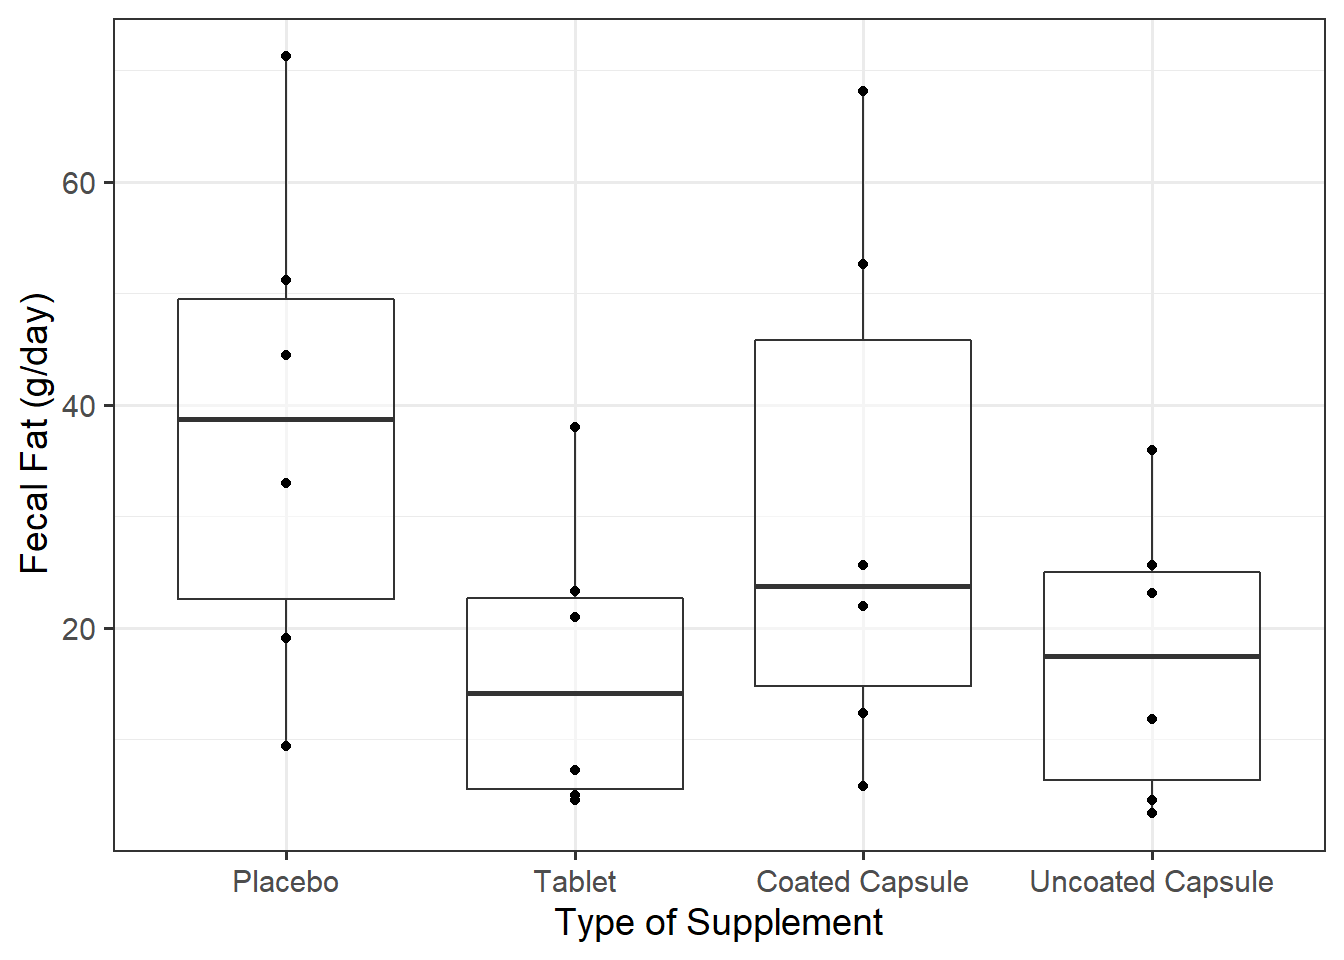
\includegraphics[width=0.8\textwidth]{./Images/rm-terminology-enzyme-plot-1} 

}

\caption{Data from a digestive enzyme study assuming 24 subjects.}\label{fig:rm-terminology-enzyme-plot}
\end{figure}

Of course, the above analysis is predicated on the data being consistent with the conditions for the classical regression model. For example, it seems reasonable to assume that the fecal fat present in one subject is independent of the fecal fat present in any other subject once we have accounted for the type of supplement. Therefore, it seems reasonable that any two fecal fat measurements above are independent once we have accounted for the type of supplement received. This, however, follows from how we assumed the data was collected --- that each measurement is from a different subject.

Let's reconsider the above example but add a little more context to the study design.

\begin{example}[Digestive Enzymes Expanded]
The \emph{Digestive Enzymes} study was designed as a cross-over study enrolling six subjects. Each subject was placed on a form of the enzyme (determined randomly) and followed for a specified period of time at which point the amount of fecal fat present was obtained. Following a substantial wash-out period the subject was assigned a different form of the supplement. This continued until each subject had been assigned to all four supplement forms. The data, with the subject identifier information is presented in Table \ref{tab:rm-enzyme-data-table-expanded}.

Interest is in determining if the amount of fecal fat produced, on average, differed for any of the treatments. However, it is known that the amount of fecal fat present can vary substantially from one individual to another due to dietary preferences; researchers would like to account for the variation in the fecal fat across subjects when performing the analysis.
\end{example}

\begin{table}

\caption{\label{tab:rm-enzyme-data-table-expanded}Data from study comparing different forms of an enzyme supplement with subject identifier information included.}
\centering
\begin{tabular}[t]{lrrrrrr}
\toprule
  & Subject 1 & Subject 2 & Subject 3 & Subject 4 & Subject 5 & Subject 6\\
\midrule
Placebo & 44.5 & 33.0 & 19.1 & 9.4 & 71.3 & 51.2\\
Tablet & 7.3 & 21.0 & 5.0 & 4.6 & 23.3 & 38.0\\
Coated Capsule & 12.4 & 25.6 & 22.0 & 5.8 & 68.2 & 52.6\\
Uncoated Capsule & 3.4 & 23.1 & 11.8 & 4.6 & 25.6 & 36.0\\
\bottomrule
\end{tabular}
\end{table}

The additional information about the study design (the cross-over study results in several measurements being taken on each subject) indicates that the observed measurements are not independent. Instead, there is a relationship between certain responses.

\begin{rmdtip}
For those familiar, you may recognize the \emph{Digestive Enzymes} example as a ``block design.'' Others may be familiar with the ``paired design,'' of which this is a generalization. While the idea is similar, the methods discussed in this text are a more inclusive approach.
\end{rmdtip}

Why would recording multiple observations on the same subject impact the condition of independence? Looking at the data reveals that the values of fecal fat vary greatly from subject to subject, ranging from 9 to 71 g/day in some cases. This could be the result of different diets; however, such dramatic differences are never noted among measurements from the same subject. That is, the variability \emph{between} subjects is substantially larger than the \emph{variability} within a subject. This makes it difficult to find the signal between the supplement forms. Ignoring this information in our previous analysis results in reduced power.

To better understand why researchers would design such a study, we review attributes of good study design. Generally speaking, there are three components to any well-designed study: replication, randomization, and comparative groups.

\begin{definition}[Replication]
Taking measurements on different subjects for which you expect the results to be similar (differences due only to natural variability).
\end{definition}

Replication allows us to estimate subject-to-subject variability. Our intuition is that more data is better; in fact, increasing the sample size (the number of \emph{unique} subjects on which we collect data) will result in less variability in our estimates. That is, the sampling distribution for these estimates will be narrower. Increased replication also leads to increased power --- the ability to detect a signal when it really exists.

\begin{definition}[Randomization]
Random sampling refers to the selection of subjects from the population at random while random allocation refers to the assignment of subjects to treatment groups at random.
\end{definition}

There are many forms of random sampling. Some sampling schemes ensure each collection of subjects is equally likely, while others ensure representation. Some sampling schemes are weighted to oversample from some subpopulation. Each scheme shares the goal of eliminating bias, making the data more representative of the target population. While random sampling is the ideal, it is not always feasible. In clinical trials, for example, patients must elect to participate, thereby making the sample not random. When a random sample is not possible, summarizing the data to ensure it is representative of the target population is critical.

There are many forms of random allocation. Some randomization schemes ensure each treatment group is equally likely, while others assign to an active treatment with a higher likelihood than the placebo. Other randomization schemes, like that mentioned in the \emph{Digestive Enzymes} example randomizes the \emph{order} of treatments. Each scheme shares the goal of eliminating confounding, allowing for causal interpretations. Whenever possible, random allocation is utilized, but it is not always feasible. Perhaps most famously, it was deemed unethical to conduct a randomized controlled trial to investigate the link between smoking and cancer. Therefore, observational studies were utilized.

\begin{definition}[Comparative Groups]
The treatment groups (factors) should be as similar as possible to reduce the inclusion of additional variation in the process.
\end{definition}

Intuitively, the less variation in the response, the easier it is to detect a signal. This leads naturally to saying that we could eliminate extraneous variability if the groups were \emph{identical}; that results in using the same subjects in multiple groups, resulting in taking repeated measurements on the subjects.

\hypertarget{studies-with-repeated-measures}{%
\section{Studies with Repeated Measures}\label{studies-with-repeated-measures}}

Studies which have repeated measurements taken on subjects typically violate the condition of independence. While the above design concepts apply broadly, the following terminology is specific to such studies.

\begin{definition}[Repeated Measures]
Data for which the observed responses can be grouped based on some nuisance variable (typically the subject itself) which captures some inherent characteristic about the subject such that observations within a group tend to be more alike than observations across groups.
\end{definition}

\begin{rmdtip}
The ``paired data'' setting (typically studied alongside the ``paired t-test'') is a special case in which there are only two observations per group.
\end{rmdtip}

As discussed in the context of the \emph{Digestive Enzymes} example above, the large variability between subjects relative to the variability within subjects can swamp out the treatment effect if not accounted for appropriately. From a more theoretical perspective, this difference in the variability induces a correlation structure among the error in the responses.

\begin{definition}[Correlation Structure]
Quantifies the strength and direction of the relationship between the errors in the observed responses.
\end{definition}

\begin{rmdkeyidea}
Ignoring the correlation structure does not tend to affect the parameter estimates, but it often affects the resulting standard errors, thereby impacting confidence intervals and p-values.
\end{rmdkeyidea}

Unfortunately, there is no way to predict if the confidence intervals will widen or narrow; similarly, we cannot predict whether the p-values are too high or too small. As a result, ignoring the correlation structure in the data can result in inappropriate inference. In order to obtain appropriate inference, we will need methods which account for this structure.

\begin{rmdkeyidea}
When the data is correlated, it must be taken into account in all aspects of the analysis, from the graphics to inference.
\end{rmdkeyidea}

In order to illustrate the impact of the correlation structure on an analysis, consider representing the data from the \emph{Digestive Enzymes} example in which we connect observations from the same subject (Figure \ref{fig:rm-terminology-enzyme-plot-extended}). While there are some exceptions, notice how the lines do not ``mix'' often; that is, some subjects tend to have less fecal fat than others, regardless of the form of the supplement given. Even visually, we see that we should not focus on the overall average for each treatment group; instead, we see that for nearly every subject, the fecal fat is reduced with the supplement (compared to placebo). It may not be immediately obvious if there is a difference among the form of the supplement, but it seems clear that having the supplement is better than not having it.

\begin{figure}

{\centering 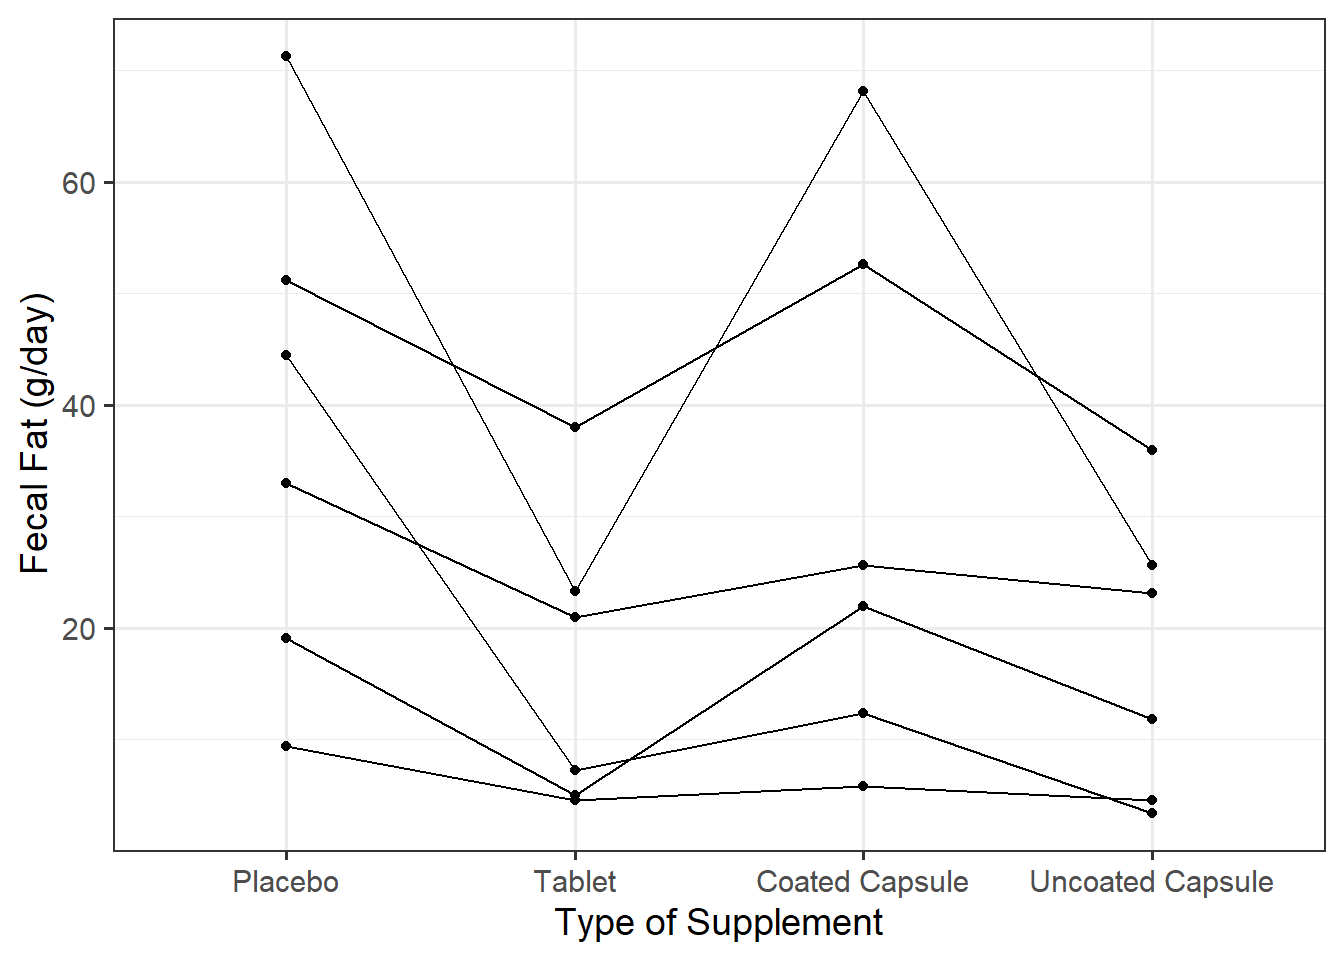
\includegraphics[width=0.8\textwidth]{./Images/rm-terminology-enzyme-plot-extended-1} 

}

\caption{Data from a digestive enzyme study involving repeated measures on six subjects.  Data from the same subject are connected to illustrate the correlation structure.}\label{fig:rm-terminology-enzyme-plot-extended}
\end{figure}

The repeated measures in the \emph{Digestive Enzymes} example is the result of blocking in order to obtain comparative groups.

\begin{definition}[Blocking]
One way of controlling for an inherent characteristic that contributes additional variation. All observations that are linked through the characteristic are grouped together and random allocation (if applicable) occurs within the block.
\end{definition}

Blocking is useful when we can identify the nuisance characteristic in advance of data collection. Blocking is a way of ensuring the treatment groups are similar because the same subjects (with respect to this particular characteristic) end up in each treatment group. We know that random allocation eliminates confounding because it ensures that, on average, treatment groups are similar. Blocking alone does not eliminate confounding; it must be combined with randomization. However, if we account for the blocking in the analysis, we are able to sharpen our estimates because not only has balance occurred, we are able to explain a portion of the variability within each treatment group.

The introduction of blocks suggests that not all ``grouping'' variables are treated the same. We think about variables differently depending on their role in the model for the data generating process. Loosely, we can categorize factors as either fixed or random effects.

\begin{definition}[Fixed Effect]
Terms in the model for which we are interested in both the specific values observed and characterizing the relationship it has with the response.
\end{definition}

In addition to the treatment/factor of interest, this can include anything we want to account for in the model in such a way that if we were to repeat the study, the same levels would be visible again. In terms of the parameters in the model, we think of the parameters as constants (though unknown) which hold true for all individuals. In the \emph{Digestive Enzymes} example, the form of the supplement is the fixed effect. If we were to repeat the study, we would still expect to use these same four levels (placebo, tablet, coated and uncoated capsule). And, we might readily believe that the difference between a placebo and a tablet is the same for all subjects.

\begin{definition}[Random Effect]
Terms in the model that capture the correlation induced due to an inherent characteristic that varies across the population and for which we are \emph{not} interested in the specific values observed or characterizing the relationship it has on the response directly.
\end{definition}

This is generally \emph{not} the treatment/factor of interest; in fact, we are rarely interested in saying how such terms directly impact the response. We believe that the variability in the response among the groups is large relative to the variability in the response within such groups. The induced correlation can therefore be partitioned out using these variables. In the \emph{Digestive Enzymes} example, the subject is a random effect. Groups of observations on the same subject are more alike than observations across subject. If we were to repeat the study, it is unlikely we would use these same six subjects. Instead, we see these subjects as representative of a random sample from some population; therefore, the difference between subjects 1 and 2 is not of real interest and would change from one study to the next.

\begin{rmdtip}
In order to distinguish fixed and random effects in a model, think about repeating the study; would you care if the levels of the factor were to change? Are you interested in comparing the first level to the second? If you answer ``yes'' to these questions, the factor is most likely a fixed effect.
\end{rmdtip}

A key idea in regression modeling is partitioning variability. The more things you can explain, the better your comparison of interest. We are removing elements from the ``junk drawer'' (the elements contributing to the error between observations). With a random effect, we are partitioning out something that we believe fluctuates and the specific values are of no interest.

In the \emph{Digestive Enzymes} example, each observation is from a unique combination of the subject on which it was observed and the treatment assigned at that time. This is not the only form of a study that can result in repeated measurements. In the biological sciences, it is common to record the response several times on the same subject.

\begin{definition}[Subsampling]
A process in which each subject has several measurements of the response taken, possibly at unique locations.
\end{definition}

In a study with subsampling, the unit of observation is the subject itself. For example, the subject is randomized to a particular treatment; however, the response of interest is measured multiple times. As an example, a person may be assigned to a particular treatment to improve eyesight. The subject's eyesight is then measured in each eye; the person is the unit of measurement but we obtain two measurements of the response (eyesight), one corresponding to each eye. This is sometimes referred to as ``pseudo-replication,'' and many researchers can mistakenly believe they have a larger sample size than exists in reality; the observations recorded on the same subject are related and should not be treated as independent observations.

Before examining methods for addressing studies with repeated measures, we need to make a clear distinction. When we use the phrase ``repeated measures,'' we mean repeatedely measuring the same response. All regression models make use of multiple variables measured on the same subject. The models discussed in this unit refer to measuring the same response repeatedly.

\hypertarget{rm-mixed-models}{%
\chapter{Mixed Effects Models}\label{rm-mixed-models}}

As we stated in the previous chapter, repeated measures induces a correlation structure on the observed data. Many scientific questions could be answered by modeling the \emph{average} response while accounting for the correlation structure when making inference. However, other questions may seek to characterize how the parameters vary across subjects in the population. In either case, considering a flexible modeling framework that builds up the data generating in stages can be helpful.

\hypertarget{partitioning-variability}{%
\section{Partitioning Variability}\label{partitioning-variability}}

In order to motivate the modeling approach developed in this chapter, we first discuss the various reasons the value of the response is not the same for all observations. By constructing this conceptual framework, we see the various sources of variability and the various ways in which the repeated observations are related with one another. This then allows us to construct a model in stages.

\begin{rmdkeyidea}
Statistical models partition variability in the response.
\end{rmdkeyidea}

We can view regression models as trying to explain why the response values differ across observations. The more reasons we can put in place, the more variability we are able to explain. This allows us to better characterize the differences we observe and more accurately make predictions. There are several sources of variability.

While these ideas generalize to many types of studies, it helps to imagine measuring the response of interest at several points across time for each subject. The observed responses may be expected to differ across time; they may also be expected to differ if they were exposed to different treatment groups or the subjects have different values of a key covariate. For example, the weight of children is expected to change as they age; further, the weight of a child may be expected to differ depending on their height. This is the overall trajectory in the population is typically what we are interested in parameterizing and making inference upon.

Of course, the trajectory of any particular subject (across their repeated observations) will differ from the overall trajectory. At any point in time, a subject may have a trajectory that is above average; others will have a trajectory that is below average. This vertical shift or ``bump'' in the position of the trajectory captures the biological variation between subjects. Of course, we could constrain whether this shift is allowed to change over time or not. All observations measured on the same subject will share a similar ``bump,'' creating a relationship between observations.

For any subject, the actual response is likely to not lie directly on their individual trajectory. For example, a child's growth may not follow a smooth growth-curve even if we model it in that way. This is the result of natural biological fluctuations from the trajectory. A child's weight on any one day bounces around their trajectory depending on their recent food intake and activity level. As such, observations measured close together in time can tend to be more alike than those measured further apart in time. As an example, if a child's weight is slightly above their individual trajectory at this moment, it is likely to be above their trajectory an hour from now. However, if a child's weight is slightly above their individual trajectory at this moment, it does not really tell us anything about whether their weight will be slightly above or below their individual trajectory a year from now. Therefore, magnitudes of this source of variability are thought to be related when close in time and independent otherwise.

Finally, it is unlikely that the observed response is equal to the \emph{actual} response as a result of measurement error. The weight of a child will be subject to the accuracy and precision of the scale, whether the subject was measured with or without clothing and shoes, etc. The magnitude of such errors are thought to be independent of one another.

This discussion highlights that the ``error'' we typically consider in a linear model is actually the result of several sources of variability. The above discussion highlights some common beliefs.

\begin{rmdkeyidea}
Observations from the same block (could be subject or other inherent grouping) tend to be high or low (relative to the average) together, incuding a ``between-subject'' correlation. It is common to think that observations from different blocks are independent.

Observations from within a block recorded close together in time are likely to be related, inducing a ``within-subject'' correlation. It is common to think that observations far apart in time are independent.
\end{rmdkeyidea}

Taking into account all sources of variability can result in a very complex model (and this continues to be an area of active research). In practice, we can make simplifying assumptions about the data generating process that allows us to rely on a simpler construct. For example, we may assume the data are collected far enough apart in time so that the within-subject correlation is negligible.

\hypertarget{model-formulation}{%
\section{Model Formulation}\label{model-formulation}}

Our discussion above illustrates how the various sources of error/variability build on one another to create the observed data. We worked backward; we started with the overall trend and decomposed it to arrive at the data observed. When we model, we work the other direction, building the model in stages. This is known as a hierarchical model.

\begin{definition}[Hierarchcial Model]
A model in which is broken into stages defining a hierarchy of units capturing the sources of variability.
\end{definition}

For our purposes, we can consider a hierarchical model that is composed of two stages: the individual and the population. In particular, we first model the trajectory within the individual (the observations within a block); then, we describe how that trajectory changes across individuals in the population (between observations in different blocks).

\begin{definition}[Individual-Level Model]
Characterizes the responses for the \(i\)-th subject (or block) only.
\end{definition}

We can often think of the individual-level model as the one we would construct if we only had data for a single subject/block. Therefore, this model can only make use of within-individual predictors --- those which vary within a subject/block. In biological settings, this is most common when measurements are taken across time; for example, following a child over several years, the height of the child will change. However, it is unlikely that the highest level of education achieved by the child's parents is likely to change. In that case, the height and time itself would be within-individual predictors, but the education level of the parents would not be.

Consider the \emph{Digestive Enzyme} Example (\ref{exm:rm-enzyme-expanded}) of the previous chapter. The individual-level model would model the fecal fat observed within a subject; we would expect the responses to differ in part because of the form of the supplement as well as measurement error. This leads to a model of the form

\[(\text{Fecal Fat})_i = \alpha_{0,i} + \alpha_{1,i} (\text{Tablet})_{i,j} + \alpha_{2,i} (\text{Coated})_{i,j} + \alpha_{3,i} (\text{Uncoated})_{i,j} + \varepsilon_{i,j}\]

where here \(i\) is indexing the subject and \(j\) the observation within each subject. It is common to take

\[\varepsilon_{i,j} \stackrel{\text{IID}}{\sim}N\left(0, \sigma^2\right).\]

This model makes use of the supplement form because it changes across the observations within a subject; it is an individual-level predictor. What is unique about this model formulation is at this point, the \emph{parameters} themselves are allowed to vary across subjects. How those vary is determined by the population-level model.

\begin{definition}[Population-Level Model]
Characterizes how the \emph{parameters} of the individual-level model vary across subjects/blocks in the population.
\end{definition}

While we do not actually proceed in this way, we can conceptualize this as the model we construct using the estimates from the \(i\) individual-level models as responses in a new model. That is, we imagine using the data from each of the \(i\) individuals to estimate the individual-level parameters; we will have \(i\) different estimates. We then feed these into a model as responses and use the characteristics of the groups to explain why these vary. This second-stage model makes use of among-individual predictors --- those which vary across subjects/blocks but are constant for all observations on the same subject/block. Often, these are the treatment groups of interest, with the exception of block designs.

For the \emph{Digestive Enzyme} example, we want to explain how (if at all) the parameters from the individual-level model vary across the subjects. There is not a single answer, but instead, the model constructed should communicate our beliefs about the data-generating process. Suppose we are willing to believe the following:

\begin{itemize}
\tightlist
\item
  The delivery of the medication affects each subject in a similar way. That is, if the tablet is best for one subject, we believe it is best for all subjects. And, the only reason it may not appear this way in the observed data is due to random noise (which we captured by \(\varepsilon_{i,j}\) in the individual-level model).
\item
  The baseline level of fat in each person is fundamentally different. That is, due to diet and genetics etc., each person has a unique level of fat. Some people have more than others, and that varies randomly in the population, but it is centered on some value.
\end{itemize}

Again, we might disagree on whether these two assumptions are appropriate, but once we agree on a set of reasonable assumptions, it guides the model. The first assumption above says that the treatment effects in the individual-level model \(\left(\alpha_{1,i}, \alpha_{2,i}, \alpha_{3,i}\right)\) are the same for every individual. The second assumption says that the intercept, the baseline level of fat under the placebo arm, differs across subjects randomly. Putting these together, the population-level model takes the form

\[
\begin{aligned}
  \alpha_{1,i} &= \beta_1 \\
  \alpha_{2,i} &= \beta_2 \\
  \alpha_{3,i} &= \beta_3 \\
  \alpha_{0,i} &= \beta_0 + b_{0, i} \\
  b_{0,i} &\sim N\left(0, \sigma^2_0\right)
\end{aligned}
\]

for some unknown \(\sigma^2 > 0\). We are modeling the intercept in the individual-level model as a random component as a result of the subjects; hence the name ``random effect.''

While we have describe the individual-level and population-level models, the combination of these is needed to fully explain the data. The idea that some of our effects (coefficients) in a model are fixed (not allowed to vary across individuals) and some are random (allowed to vary across individuals) leads to our description of this model as a mixed-effects model.

\begin{definition}[Mixed Effects Model]
A model which contains both fixed and random effects. Useful for modeling repeated measures from a hierarchical perspective.
\end{definition}

It can be useful to represent the mixed-effects model in a combined model instead of its individual components. For the \emph{Digestive Enzyme} example, we simply substitute the population-level model into the individual-level model. This results in

\[
\begin{aligned}
  (\text{Fecal Fat})_{i,j} 
    &= \left(\beta_0 + b_{0,i}\right) + \beta_1 (\text{Tablet})_{i,j} + \beta_2 (\text{Coated})_{i,j} + \beta_3 (\text{Uncoated})_{i,j} + \varepsilon_{i,j} \\
  \varepsilon_{i,j} &\stackrel{\text{IID}}{\sim}N\left(0, \sigma^2\right) \\
  b_{0,i} &\stackrel{\text{IID}}{\sim}N\left(0, \sigma^2_0\right).
\end{aligned}
\]

\begin{rmdtip}
Specifying the mixed-effects model as a single model can help with specifying the model in statistical software.
\end{rmdtip}

\begin{rmdwarning}
Proper inference in mixed-effects models is debated among statisticians. The two leading statistical software packages (SAS and R) disagree in implementation. SAS provides default p-values for each fixed-effect parameter; R does not.
\end{rmdwarning}

Despite the fully parametric nature of a mixed-effect model, inference on the fixed effects is generally carried out using large-sample theory. Generally, we do not test the random effects. Instead, we leave them in the model to capture the correlation we believe is present in the data. As a way of illustrating that incorporating the correlation structure can impact the results, the p-value for comparing the supplement forms went from 0.1682 when we did not account for the correlation to \ensuremath{3\times 10^{-4}} when we fit the mixed-effects model.

\hypertarget{considerations-when-building-a-mixed-effects-model}{%
\section{Considerations when Building a Mixed-Effects Model}\label{considerations-when-building-a-mixed-effects-model}}

Constructing a mixed-effects model can feel overwhelming at times. We urge you to keep the following ideas in mind:

\begin{itemize}
\tightlist
\item
  Construct a model that preserves the behavior at the individual-level. This is generally the stage in which we have more scientific intuition.
\item
  All the behavior to vary across subjects, which corresponds to allowing the parameters to vary. Choose which parameters to vary based on discipline expertise.
\item
  The variation in the parameters naturally induces a correlation structure in the data.
\end{itemize}

In the above discussion, we considered the error term at the individual-level model to be independent and identically distributed. In theory, we could allow a correlation to exist here as well; for example, we may want observations closer together in time to be correlated. This can dramatically increase the complexity of the model fit and often requires custom software.

When representing data from a repeated-measures study, it is useful to convey the correlation structure in the graphic. This is not always straight-forward. When the number of subjects in the study is not overwhelming, a spaghetti plot can be useful. While we made use of such a plot in the \emph{Digestive Enzyme} example in the previous chapter, these are particularly useful for studies which follow subjects over time and illustrate the trend.

\begin{definition}[Spaghetti Plot]
A scatterplot that displays the trends within a subject, highlighting the correlation structure by connecting points from the same subject.
\end{definition}

Before closing this chapter, we address the conditions of a mixed-effects model. We have the same conditions on the individual-level model as we do in classical regression models. Further, they can be assessed and relaxed in the same way. However, the conditions on the random effects are not easily assessed. In particular, the distributional assumption of Normality for the random effects is rarely questioned. Bootstrap algorithms for such processes need to be custom-written to take advantage of the hierarchy, and there is ongoing research on the efficacy of this approach.

In this text, our emphasis is on understanding and interpreting such models. Other texts consider the theoretical underpinnings of such model in more detail.

\hypertarget{rm-gee}{%
\chapter{Generalized Estimating Equations}\label{rm-gee}}

In the previous chapter, we addressed the correlation structure present in repeated measures data by developing a hierarchical model in stages. However, the correlation structure was a by-product. That is, we did not model it directly; instead, by first describing the individual-level model, and then allowing the parameters of that model to vary across individuals in the population, the correlation structure was handled naturally. In this chapter, we consider an alternate approach in which we model the correlation structure directly. This is common in longitudinal studies.

\begin{definition}[Longitudinal Study]
A study which involves repeatedly measuring the response on each subject at various points in time.
\end{definition}

All clinical trials follow subjects over time; a longitudinal study measures the response of interest multiple times over the course of the trial, resulting in repeated measures. In a longitudinal study, interest is often in modeling the overall trajectory across subjects instead of the trajectory for subjects individually. There are many similarities between longitudinal studies and time-series data as each follows data over time. We do see some differences. Time-series data is often focused on business applications while longitudinal studies are more common in the biological sciences. Time-series data often models a single ``stream'' that is quite long. Longitudinal studies have several ``streams'' (one for each subject), but these tend to be a bit shorter as we do not have constant follow-up. In time-series data, it is often believed that the previous response is useful in predicting the next response; in longitudinal data, we do believe there is correlation among the errors in the model, but we do not generally use the value of the previous observation itself in making the next prediction but instead model with time as the predictor.

\hypertarget{correlation-structrues}{%
\section{Correlation Structrues}\label{correlation-structrues}}

In Chapter \ref{rm-terminology} we defined the correlation structure as a summary of the relationship among the errors in the responses. In a mixed effects model, we considered the various sources of variability as contributing to the correlation structure; in this chapter, we are interested in modeling the structure directly. As a result, we are interested in the overall impact of the sources of variability on this structure. By specifying this structure, at least approximately, we are able to adjust the inference in our mean model to obtain appropriate inference.

We can think of the correlation on the error terms of our model to be a combination of between-subject and within-subject sources of variability. While we may not be discussing the specific sources of variability, they are just as important as before as they help us to determine an appropriate form of the correlation structure. We are generally willing to assume that observations from different subjects/blocks are independent; therefore, when we describe the correlation structure of the errors, we need only focus on the correlation of the observations from the same subject/block. Further, we assume that the correlation strucutre is the same for every subject. Therefore, there is only one correlation structure to be specified, and it will be shared across all subjects/blocks.

Recall from your introductory course that a correlation coefficient must be between -1 and 1. It captures the strength and direction of the linear relationship between two values. If each subject/block has five observations (for example), then we need to describe the relationship between any pair of these five observations. That is \(\binom{5}{2} = 10\) correlation coefficients. This is typically stored in a matrix

\[\Gamma = \begin{pmatrix} 
1 & \rho_{1,2} & \rho_{1,3} & \rho_{1,4} & \rho_{1,5} \\
\cdot & 1 & \rho_{2,3} & \rho_{2,4} & \rho_{2,5} \\
\cdot & \cdot & 1 & \rho_{3,4} & \rho_{3,5} \\
\cdot & \cdot & \cdot & 1 & \rho_{4,5} \\
\cdot & \cdot & \cdot & \cdot & 1 \end{pmatrix}.\]

\begin{rmdkeyidea}
All correlation matrices share some basic properties:

\begin{enumerate}
\def\labelenumi{\arabic{enumi}.}
\tightlist
\item
  It will be a square matrix, and the dimension is determined by the number of obsrevations within a subject/block.
\item
  A correlation matrix is symmetric (the transpose is the same as the original matrix). As a result, we do not specify the bottom half of the matrix because it can be determined by the upper half of the matrix.
\item
  The diagonal entries are always 1; any value is perfectly correlated with itself.
\item
  All off-diagonal elements must be between -1 and 1.
\end{enumerate}
\end{rmdkeyidea}

A correlation matrix is very similar to a variance-covariance matix; in fact, we can think of a correlation matrix as a standardized variance-covariance matrix. In the above example, each off-diagonal element is free to take on any value. This is called an unstructured form.

\begin{definition}[Unstructured Correlation Structure]
An unstructured correlation structure suggests that the correlation between any two errors within a subject/block can take on any value. We only require that it be a valid correlation matrix.
\end{definition}

If we think of each correlation as an additional parameter to estimate, then we have just specified an additional \(\binom{m}{2}\) parameters to our model, where \(m\) is the number of repeated observations on a subject/block. We are essentially choosing not to place any structure on the correlation matrix and allow the data to completely determine the structure. This can be useful if we have no intuition about the sources of variability; however, it requires a lot of data as we have added a large number of parameters to the model.

As in any model, there is tension between specifying a model which is flexible and one which is more tractable. We often impose some simplifying structure on the correlation matrix. While there are several possible structures, we discuss the most common. On the other extreme from the unstructured correlation matrix discussed above is to assume the observations within a subject/block are independent of one another.

\begin{definition}[Independence Correlation Structure]
No correlation among any of the error terms within a subject/block. If there are five observations within a block, this has the form

\[\Gamma = \begin{pmatrix} 
1 & 0 & 0 & 0 & 0 \\
\cdot & 1 & 0 & 0 & 0 \\
\cdot & \cdot & 1 & 0 & 0 \\
\cdot & \cdot & \cdot & 1 & 0 \\
\cdot & \cdot & \cdot & \cdot & 1 \end{pmatrix}.\]
\end{definition}

While we already assume that observations between subjects/blocks are independent, this goes further and essentially says all observations are independent. At first glance, this would seem to revert back to the classical regression model, which we have already established is inappropriate for repeated measures. However, we will argue later that using such a structure does have some differences.

When we feel that observations from the same subject/block are associated primarily because they are from the same subject/block, and that the order of the observations within the subject/block is irrelevant, a compound symmetric correlation structure is appropriate.

\begin{definition}[Compound Symmetric Correlation Structure]
Also called \emph{exchangeable}, this suggests the correlation between any two errors within a subject/block is equal. If there are five observations within a block, this has the form

\[\Gamma = \begin{pmatrix} 
1 & \rho & \rho & \rho & \rho \\
\cdot & 1 & \rho & \rho & \rho \\
\cdot & \cdot & 1 & \rho & \rho \\
\cdot & \cdot & \cdot & 1 & \rho \\
\cdot & \cdot & \cdot & \cdot & 1 \end{pmatrix}.\]
\end{definition}

The compound symmetric structure adds only one additional parameter to our model and actually models well a great many scenarios. When we do believe that the order of the observations within a subject/block is important, and that observations occurring closer together (generally in time) are more highly correlated than subjects further apart in time, an autoregressive structure is appropriate.

\begin{definition}[Autoregressive Correlation Structure]
The autoregressive structure suggestst that the correlation between two observations diminishes as the observations get further apart in time. We generally only consider the autoregressive structure of degree 1 here; if there are five observations within a block, this has the form

\[\Gamma = \begin{pmatrix} 
1 & \rho & \rho^2 & \rho^3 & \rho^4 \\
\cdot & 1 & \rho & \rho^2 & \rho^3 \\
\cdot & \cdot & 1 & \rho & \rho^2 \\
\cdot & \cdot & \cdot & 1 & \rho \\
\cdot & \cdot & \cdot & \cdot & 1 \end{pmatrix}.\]
\end{definition}

This structure is borrowed from the time-series literature. It is primarily useful when we are taking observations somewhat close together in time. Like the compound symmetric structure, it only adds a single parameter to the model.

Regardless of which of the structures we believe is beneath the data, we also assume stationarity.

\begin{definition}[Stationarity]
This assumption states that the correlation structure does not depend on time, only the distance between the observations.
\end{definition}

Essentially, at no point did we say that the structure evolves as the study continues or did we include a parameter such as \(\rho^{(\text{time})}\).

Choosing an appropriate structure is often guided by discipline expertise regarding how the sources of variability combine and impact the relationship between the responses. However, it turns out that the choice of the structure need not have a large impact on the analysis --- simply indicating in the analysis that there is a potential for correlation can be sufficient. This is the idea behind the approach we describe.

\hypertarget{the-key-to-success-of-generalized-estimating-equations}{%
\section{The Key to Success of Generalized Estimating Equations}\label{the-key-to-success-of-generalized-estimating-equations}}

In the previous section, we considered models for the correlation structure that results from the combination of the various sources of variability in the data-generating process. This structure will be used within the generalized estimating equation (GEE) approach.

\begin{definition}[Generalized Estimating Equations (GEE)]
An approach to repeated measures which focuses on modeling the parameters in the mean model while specifying a model for the correlation structure. This structure is updated during the estimation process and used to adjust the standard errors of the parameter estimates for the mean model.
\end{definition}

Recall that our inference on the parameters requires us to compute the variance-covariance matrix of the corresponding parameter estimates. For the GEE approach, the model we specify for the correlation structure is known as the ``working'' correlation matrix; this is then updated using the observed data when computing the variance-covariance matrix. As a result, the variance-covariance matrix we use is not based solely on the specified model but is a blend of the model specified and the observed data; this is known as the robust sandwich estimator.

\begin{definition}[Robust Sandwich Estimator]
An estimate of the variance-covariance matrix of the parameter estimates from the mean model. This balances the relationship between the parameter estimates specified by the model (and the ``working'' correlation matrix) with the relationship suggested by the observed data. Specifically, it has the form

\[\widehat{\boldsymbol{\Sigma}} = \widehat{\mathbf{U}} \widehat{\mathbf{U}}^{-1/2} \mathbf{R} \widehat{\mathbf{U}}^{-1/2} \widehat{\mathbf{U}}\]

where \(\mathbf{U}\) represents the model-based variance-covariance matrix if the structure specified by the working correlation matrix were completely correct, and \(\mathbf{R}\) represents the correction factor estimated from teh residuals which is an empirical estimate.
\end{definition}

\begin{rmdkeyidea}
The use of the robust sandwich variance-covariance estimator is what makes the GEE approach unique and so powerful.
\end{rmdkeyidea}

While the structure of \(\mathbf{U}\) is beyond the scope of the course, we can think of it as what the computer does by default when we specify a model under the classical conditions. Essentially, the use of the robust sandwich estimator in the GEE framework means our posited correlation structure need not be correct; it is okay if \(\mathbf{U}\) is wrong. With enough data, the inference will be the same regardless of the structure we choose. What we are really specifying is that there is a potential for correlation among these observations. Of course, the better the specified model for the correlation structure, the less adjustment that is needed and the more powerful the results.

\begin{rmdtip}
It is the use of the robust-sandwich estimator that makes specifying the ``independent'' correlation structure different than assuming the classical regression model. In classical regression, inference is based on assuming independence. In a GEE framework, the correlation structure will be updated after we assume independence.
\end{rmdtip}

\begin{rmdtip}
While we are discussing the use of the robust-sandwich estimator as a way of adjusting for the correlation present, we note that this will also adjust for violations in constant variance as a result.
\end{rmdtip}

\hypertarget{comparison-of-gee-and-mixed-effects-approaches}{%
\section{Comparison of GEE and Mixed Effects Approaches}\label{comparison-of-gee-and-mixed-effects-approaches}}

While both mixed effects models and estimation via generalized estimating equations account for the correlation structure, the two approaches differ in many ways. The mixed effects modeling approach is fully parametric, while estimating via GEE is semi-parametric; instead, inference is based on large-sample theory.

More broadly, these represent two different approaches to repeated measures data: subject-specific and population-averaged.

\begin{definition}[Subject Specific Models]
Also known as conditional modeling, this approach models at the subject-level and addresses the correlation indirectly through the inclusion of random effects.
\end{definition}

\begin{definition}[Population Averaged Models]
Also known as marginal modeling, this approach considers a model for the mean response directly and addresses the correlation through directly modeling the structure.
\end{definition}

\hypertarget{part-nonlinear-models}{%
\part{Nonlinear Models}\label{part-nonlinear-models}}

\hypertarget{nlm-framework}{%
\chapter{Nonlinear Model Framework}\label{nlm-framework}}

In Chapter \ref{glm-splines} we saw that linear models are those which are linear in their \emph{parameters}. Further, the linear model is flexible enough to capture various forms of curvature. However, models which are nonlinear in the parameters often develop from scientifically modeling processes in chemical engineering, ecology, and cellular biology. Further, when the response is a categorical variable instead of quantitative, the most appropriate models are often nonlinear in the parameters. While the general linear modeling framework is flexible enough to be used to capture the observed relationships, nonlinear models allow us to embed the scientific parameters into a statistical framework.

We motivate this unit by considering the pharmacokinetics (how a drug is processed by the body) of an anti-asthmatic agent known as Theophylline.

\begin{example}[Pharmacokinetics of Theophylline]
An early-phase clinical study was conducted to assess how Theophylline (an anti-asthmatic agent) is absorbed and eliminated from the human body. A single subject was given an oral dose of 4 mg of the drug, and 11 blood samples were taken over the course of a 24 hour period to determine the concentration of the drug in the body. A graphical summary of the resulting data is presented in Figure \ref{fig:nlm-theoph-plot}.
\end{example}

\begin{figure}

{\centering 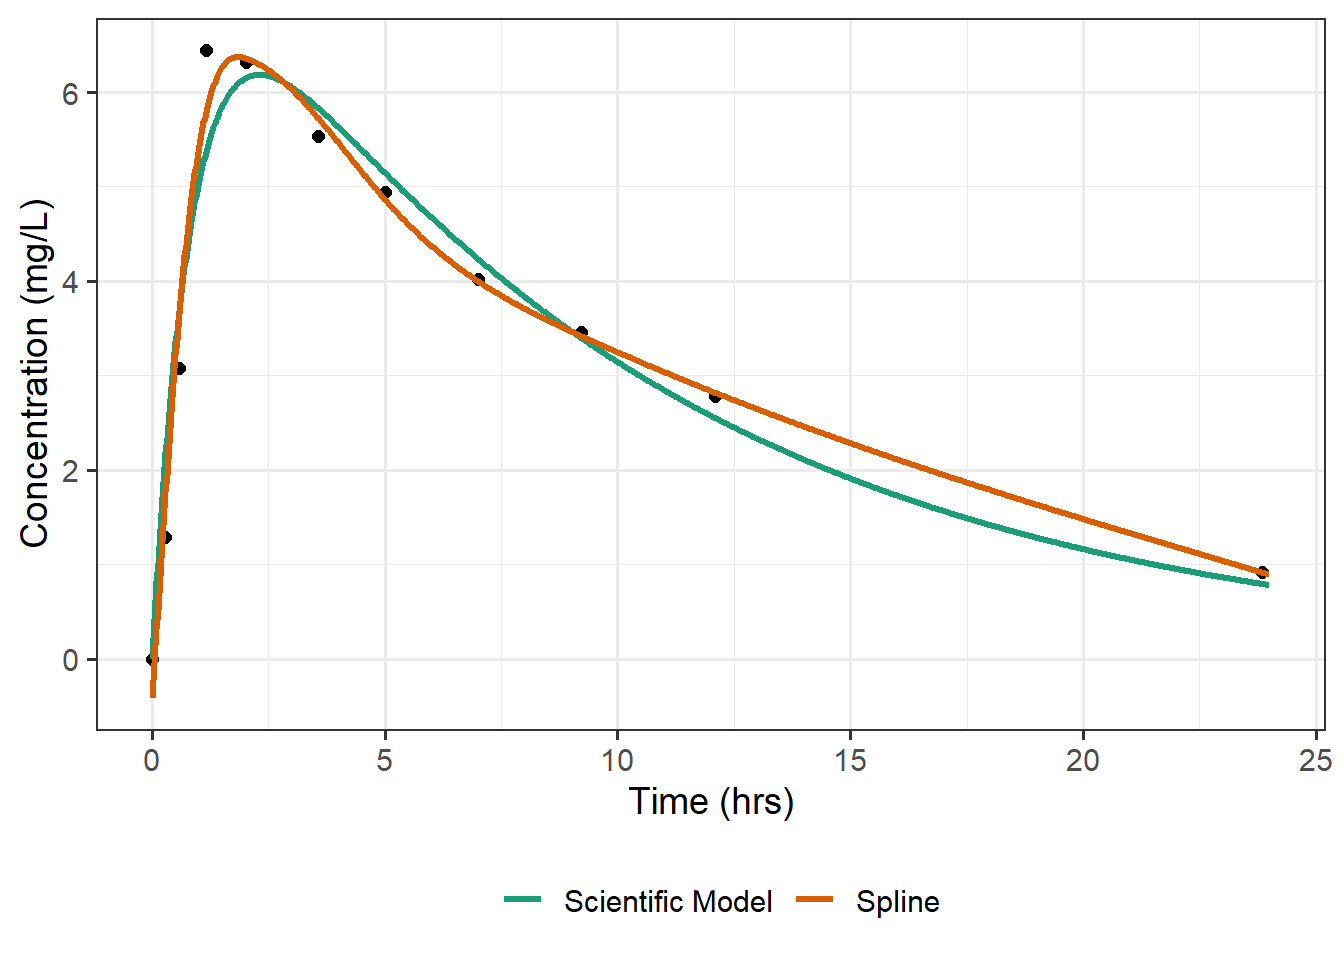
\includegraphics[width=0.8\textwidth]{./Images/nlm-theoph-plot-1} 

}

\caption{Concentration of Theophylline in the blood stream over a 24-hour period.}\label{fig:nlm-theoph-plot}
\end{figure}

We might first consider using a flexible spline in order to model the relationship. From the graphic, we note that such a fit performs rather well. However, though we were able to predict well, it does not really address the question of interest: how quickly is this drug absorbed and eliminated from the system? That is, this initial modeling approach does not lend itself to expressing the question of interest as a statement about the parameters in the model. It also separates the data analysis from the scientific modeling.

\begin{rmdkeyidea}
Nonlinear models are often the result of embedding a scientific model in a statistical framework.
\end{rmdkeyidea}

\hypertarget{scientific-model-for-theophylline}{%
\section{Scientific Model for Theophylline}\label{scientific-model-for-theophylline}}

We illustrate how the scientific model for the pharmicokinetics of Theophylline suggest a nonlinear model. Readers who are not familiar with differential equations can skip this section without loss of continuity.

Researchers believe that the absorption and elimination of Theophylline can be modeled using a one-compartment open model with first order absorption, represented by Figure \ref{fig:nlm-Theophylline-Model}. The box represents the ``blood compartment.'' The drug is absorbed into the blood stream through the gut; it is then metabolized by the liver and excreted by the kidneys.

\begin{figure}

{\centering 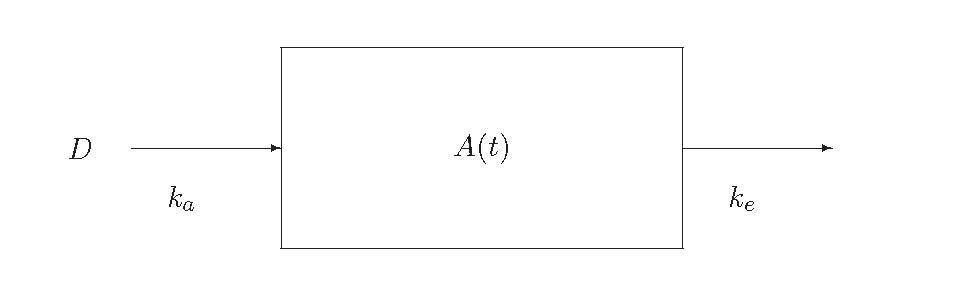
\includegraphics[width=0.8\textwidth]{images/Theophylline-Model} 

}

\caption{Scientific model for pharmicokinetics of Theophylline.}\label{fig:nlm-Theophylline-Model}
\end{figure}

Mathematical modeling allows us to characterize the concentration of Theophylline in the blood over time as a function of the elimination rate, the absorption rate, and the clearance rate (measures volume of blood cleared of the drug per unit time). Let \(D\) represent the oral dose given at time \(t = 0\); as the subject has not been given the treatment prior, it is reasonable to assume that the amount of drug in the blood \(A(t)\) initially is 0 mg; that is, \(A(0) = 0\). Further, researchers believe the body can absorb the entire dose \(D\); therefore, the amount of drug at the absorption site \(A_a(t)\) is initially \(D = 4\) mg; that is, \(A_a(0) = D = 4\). Letting \(k_a\) and \(k_e\) represent the absorption and elimination rates, respectively, we have the following mathematical model corresponding to the above scientific model:

\[
\begin{aligned}
  \frac{d}{dt} A(t) &= k_a A_a(t) - k_e A(t) \\
  \frac{d}{dt} A_a(t) &= -k_a A_a(t).
\end{aligned}
\]

Scientists believe that the amount of drug in the blood stream at any time is proportional to the concentration of the drug at that time \(C(t)\). That is, \(A(t) = V C(t)\), where \(V\) represents the volume of the blood compartment. The above system of differential equations can be solved using Laplace transforms. Letting \(V = \beta/k_e\) where \(\beta\) is the clearance rate, we are led to the following solution:

\[C(t) = \frac{k_a D}{\left(\beta/k_e\right)\left(k_a - k_e\right)} \left(e^{-k_e t} - e^{-k_a t}\right).\]

What we want to emphasize is that the form of the model for the concentration of the drug in the body was not developed empirically using statistical modeling techniques; instead, it was derived through mathematical modeling of the drug itself from scientific principles. The parameters of the model \(k_a\), \(k_e\), and \(\beta\) are unknown bug govern the process. More, these parameters are directly related to the scientific question of interest. We can now embed this scientific model into a statistical framework (accounting for sources of variability) in order to make inference on the parameters.

\hypertarget{nonlinear-regression-model}{%
\section{Nonlinear Regression Model}\label{nonlinear-regression-model}}

We take a semiparametric modeling perspective for developing our framework. Under this approach, we employ the strategy of least squares to obtain our estimates and apply large sample theory to characterize the sampling distributions of our our estimates. This framework is quite flexible.

\begin{definition}[Nonlinear Model]
A regression model that is \emph{not} linear in the parameters.
\end{definition}

Consider the scientific model for Theophylline:

\[C(t) = \frac{k_a D}{\left(\beta/k_e\right)\left(k_a - k_e\right)} \left(e^{-k_e t} - e^{-k_a t}\right);\]

there is no way of rewriting this model as a linear combination of the parameters \(k_a\), \(k_e\), and \(\beta\).

\begin{rmdtip}
When your model has more parameters than predictors, you likely have a model which is nonlinear in the parameters.
\end{rmdtip}

Our semiparametric approach, also known as a \emph{moment model}, focuses on specifying the mean and variance of the response given the predictors.

\begin{definition}[Nonlinear Regression Model]
We specify the nonlinear model in terms of the \emph{mean} and \emph{variance} of the response given the predictors; specifically,

\[
\begin{aligned}
  E\left[(\text{Response})_i \mid (\text{Predictors})_i\right] 
    &= f\left((\text{Predictors})_i, \boldsymbol{\beta}\right) \\
  Var\left[(\text{Response})_i \mid (\text{Predictors})_i\right]
    &= \sigma^2
\end{aligned}
\]

where \(f(\cdot)\) is referred to as the mean response function.
\end{definition}

Notice that under this specification there is no ``error'' term. We only concern ourselves with positing the mean and variance; not only do we not specify the distribution of the ``errors,'' we do not even make use of them in our conceptualization of the model. We note that some authors choose to specify the model as

\[(\text{Response})_i = f\left((\text{Predictors})_i, \boldsymbol{\beta}\right) + \varepsilon_i\]

and sometimes go on to assume \(\varepsilon_i \stackrel{\text{IID}}{\sim}N\left(0, \sigma^2\right)\). However, this approach is not as flexible. First, it requires the response to be quantitative. By only specifying the mean and variance of the response, our approach generalizes to accommodating categorical responses (though we focus on quantitative responses for the majority of this unit). Second, there is little to be gained by a fully parametric approach as this does not avoid the requirements for large sample theory as it does in the linear model case.

Finally, we note that in our specification above, we have assumed the variability of the response is constant for all values of the predictor. We will relax this condition in a later chapter.

It should be noted that in some cases, the mean response function \(f(\cdot)\) lends itself to a transformation that results in a linear model. For example, if \(f(x, \boldsymbol{\beta}) = \beta_0 e^{\beta_1 x}\), then taking the natural logarithm of both sides results in a linear model: \(\ln\left(\beta_0\right) + \beta_1 x\). As a result, in some disciplines, it is standard practice to consider such transformation prior to modeling. There is not widespread agreement in the statistical community on such transformations.

\begin{rmdwarning}
There is a difference between taking nonlinear transformations of a predictor to fit curvature in a linear model and taking nonlinear transformations of a model (the response often) in order to convert a nonlinear model into a model which is linear with respect to some function of the parameters.
\end{rmdwarning}

Applying some function so that the model is linear in the parameters (or at least, some function of the parameters) allows standard software to be used. As scientists are familiar with approaches for fitting linear models, this often makes it easy to put in a context that is understood. However, such transformations may destroy other modeling conditions, such as that of constant variance (or any distributional assumptions, if applicable). Transformations can also result in the model no longer being parameterized by the scientific quantities of interest. As scientific principles often directed the development of the nonlinear model, this is the scale on which scientists have intuition (it may be more difficult to think on the logarithmic-scale, for example), meaning scientists have less intuition on the transformed scale. Finally, there are some models for which such a transformation is not possible. As a result, we argue for using the nonlinear regression framework and studying methods for fitting such models.

\hypertarget{estimation}{%
\section{Estimation}\label{estimation}}

Estimation is performed analogous to what occurs in the general linear model framework. That is, we consider the optimization problem of choosing the parameters to ensure the predicted mean function is as close to the observed responses as possible.

While we do not have an error term in the model, we can still consider the residuals when motivating a method for estimating the parameters. The least squares estimates minimize

\[\sum\limits_{i=1}^{n} \left[(\text{Response})_i - f\left((\text{Predictors})_i, \boldsymbol{\beta}\right)\right]^2.\]

In the nonlinear model literature, this is often referred to as the \emph{ordinary} least squares estimator. Note that if we take \(f(\cdot)\) to be a linear function in the parameters, then the linear model framework is a special case of the nonlinear regression model. This estimation procedure is performed numerically; further details are provided at the end of this unit.

Given parameter estimates, we can then estimate the residual variance:

\[\widehat{\sigma}^2 = \frac{1}{n-p} \sum\limits_{i=1}^{n} \left[(\text{Response})_i - f\left((\text{Predictors})_i, \widehat{\boldsymbol{\beta}}\right)\right]^2\]

where \(p\) represents the number of \emph{parameters} in the model, which need not correspond to the number of predictors in a nonlinear model.

As with previous models discussed in the text, the process of estimating the parameters is a mathematical problem. It is the process of making inference in which we move into the realm of statistics.

\hypertarget{inference-on-the-parameters}{%
\section{Inference on the Parameters}\label{inference-on-the-parameters}}

In order to make inference about the parameters, we need a model for the sampling distribution of the parameter estimates. Unlike previously, we cannot rely on probability theory to obtain exact models for the sampling distributions. Therefore, we rely on large-sample theory and empirical models.

\begin{definition}[Large Sample Sampling Distribution of Parameter Estimates in Nonlinear Models]
Assuming the form of the model is correctly specified with parameter vector \(\boldsymbol{\beta}\), as the sample size gets large, we have that

\[\frac{\widehat{\beta}_j - \beta_j}{\sqrt{Var\left(\widehat{\beta}_j\right)}} \sim N(0, 1)\]

for all \(j = 1, \dotsc, p\). Further, under the null hypothesis

\[H_0: \mathbf{K}\boldsymbol{\beta} = \mathbf{m}\]

we have

\[\left(\mathbf{K}\widehat{\boldsymbol{\beta}} - \mathbf{m}\right)^\top \left(\mathbf{K}\widehat{\boldsymbol{\Sigma}}\mathbf{K}^\top\right)^{-1} \left(\mathbf{K}\widehat{\boldsymbol{\beta}} - \mathbf{m}\right) \sim \chi^2_r\]

where \(r\) is the rank (number of rows) of \(\mathbf{K}\).
\end{definition}

\begin{rmdtip}
Large sample theory is often relied on regardless of the sample size. It is often the case that there is so little error in the responses that the sampling distributions of the estimates comes close to these asymptotic approximations with little data.

Making additional distributional assumptions does not avoid the need for large sample theory.
\end{rmdtip}

The above results allow us to not only construct confidence intervals, but we can also make use of the general linear hypothesis testing framework for testing specific hypotheses. That is, our inference is not all that different than under the linear model framework once we have estimates for the parameters and estimates for their standard errors.

\hypertarget{allowing-relationships-to-vary-across-groups}{%
\section{Allowing Relationships to Vary Across Groups}\label{allowing-relationships-to-vary-across-groups}}

Modeling involves positing a relationship between the response and the predictors. Suppose we believe the form of the model is similar for all subjects in a population, but the specific parameters may differ across sub-populations. By including interaction terms, we can allow the relationship to vary across sub-populations.

\begin{rmdkeyidea}
Interaction terms allow a parameter to vary depending on the value of another variable.
\end{rmdkeyidea}

The idea of allowing a relationship to depend upon a predictor is something we have studied in each of the previous units. The same ideas apply in nonlinear models; the difference is that computationally, it requires more to specify the model appropriately in the computer.

\begin{rmdtip}
In order to allow parameters to vary across various sub-populations, consider the following:

\begin{itemize}
\tightlist
\item
  Refine your question in terms of which parameters will be allowed to vary, and which parameters will remain fixed for all groups.
\item
  Use an indicator variable to capture the grouping structure.
\item
  If necessary, obtain starting values by fitting separate models to subsets of the data.
\item
  Embed your research question into the general linear hypothesis framework.
\end{itemize}

These considerations are quite general and can be widely applied.
\end{rmdtip}

As an example, suppose that we believe that, in general, a particular bacteria grows exponentially. That is, we believe the response has the following \emph{form}:

\[E\left[(\text{Response})_i \mid (\text{Time})_i\right] = \beta_0 + e^{\beta_1 (\text{Time})_i}.\]

Suppose we grow this bacteria in two different media. While wells containing the bacteria are seeded at the same amount regardless of the media (same amount of bacteria to begin with), we believe the media might result in different growth rates. As a result, we expect the value of \(\beta_0\) to be the same for both media, but the value of \(\beta_1\) could differ for the two groups. We model this using an interaction term. Define an indicator variable

\[(\text{Media B})_i = \begin{cases} 1 & \text{if i-th observation grown with media B} \\ 0 & \text{if i-th observation grown with media A} \end{cases}.\]

Now, consider the following model:

\[E\left[(\text{Response})_i \mid (\text{Time})_i, (\text{Media})_i\right] = \gamma_0 e^{\left(\gamma_1 + \gamma_{2} (\text{Media B})_i\right) (\text{Time})_i} = \gamma_0 e^{\gamma_1 (\text{Time})_i + \gamma_{2} (\text{Media B})_i (\text{Time})_i}.\]

This model has an interaction between \texttt{Media\ B} and \texttt{Time}; however, there is no ``main effect'' of \texttt{Media\ B}. Again, this single model implies expected responses for each media:

\[
\begin{aligned}
  \text{Media A}&: E\left[(\text{Response})_i \mid (\text{Time})_i\right] = \gamma_0 + e^{\gamma_1 (\text{Time})_i} \\
  \text{Media B}&: E\left[(\text{Response})_i \mid (\text{Time})_i\right] = \gamma_0 + e^{\left(\gamma_1 + \gamma_2\right)(\text{Time})_i}.
\end{aligned}
\]

Notice this maintains the assumptions we had about the process:

\begin{itemize}
\tightlist
\item
  The initial state is the same under both media \(\left(\gamma_0\right)\).
\item
  The growth rate is allowed to differ under the two media.
\end{itemize}

As discussed when we introduced interaction terms in linear models, the benefits of using interaction terms instead of doing a subgroup analysis is that we can easily control which parameters are allowed to differ, we make use of the constant variance condition gaining power, and our question of interest is embedded in the model. To illustrate this last point, notice that the hypotheses

\[H_0: \gamma_2 = 0 \qquad \text{vs.} \qquad H_1: \gamma_2 \neq 0\]

test whether the growth rate actually differs between the two media.

\hypertarget{nlm-heteroskedasticity}{%
\chapter{Relaxing the Constant Variance Condition}\label{nlm-heteroskedasticity}}

When describing the nonlinear modeling framework, our most limiting assumption was that of constant variance. In Chapter \ref{rm-gee}, we saw one method of handling non-constant variance (the robust sandwich variance-covariance estimator). In this chapter, we discuss other approaches for relaxing the assumption of constant variance. While we introduce them in the context of nonlinear models, they are applicable to a wider range of models including linear models and models for addressing repeated measures.

\hypertarget{modeling-assumptions}{%
\section{Modeling Assumptions}\label{modeling-assumptions}}

The previous chapter focused on the mechanics of specifying and fitting nonlinear models. But, we only mentioned the conditions on the model. The semiparametric approach does place conditions on the model.

\begin{definition}[Conditions on the Nonlinear Model]

\begin{itemize}
\tightlist
\item
  The mean response function is correctly specified.
\item
  Given the value of the predictors, any two observations are independent.
\item
  The variability of the response is the same for all values of the predictor.
\end{itemize}

\end{definition}

These are essentially the same first three conditions we imposed in the linear model framework (which should not be a surprise since the linear model framework is a special case of the nonlinear model we specified). As a result, these conditions can be assessed in much the same way - residual plots. Specifically, a plot of the residuals against the predicted values can be used to assess whether the mean response function is correctly specified. We expect the residuals to balance out at 0 for each predicted value. This helps to assess if the process is behaving according to the scientific model. When the order of the data is known, we can use a time-series plot of the residuals to examine deviations from the independence condition over time. If independence is reasonable, we expect the residuals to display no trends in location or spread over time. We can assess constant variance by examining a plot of the residuals against the predicted values; we would expect the spread of the residuals to be constant as we move left-to-right across the plot.

\begin{rmdtip}
Nonlinear modeling applications often have small sample sizes. As a result, it can be difficult to assess constant variance from the plot of the residuals against the fitted values. A ``trick'' is to plot the absolute value of the residuals against the fitted values. This ``doubles'' the visual information in the graphic and can allow us to more easily pick up trends in the spread.
\end{rmdtip}

While we do not assume the response (condition on the predictors) follows a Normal distribution, if we had, we could assess this condition using a probability plot of the residuals.

\begin{example}[Pharmacokinetics of Indomethacin]
Indomethacin is an NSAID pain reliever used to treat severe pain and prevent premature labor in some cases. A study was conducted to examine the pharmacokinetic properties of the drug. Indomethacin is given as an IV-bolus and travels through the blood and deeper tissues. Scientists model this as a two-compartment open model, which leads to the following nonlinear model for the concentration \(C(t)\) of the drug at any time \(t\):

\[C(t) = \beta_1 e^{-\beta_2 t} + \beta_3 e^{-\beta_4 t}\]

which is also known as the bi-exponential model. Blood samples were taken from a single subject after being given an IV-bolus of the drug. The data is shown in Figure \ref{fig:nlm-indomethacin-plot}.
\end{example}

\begin{figure}

{\centering 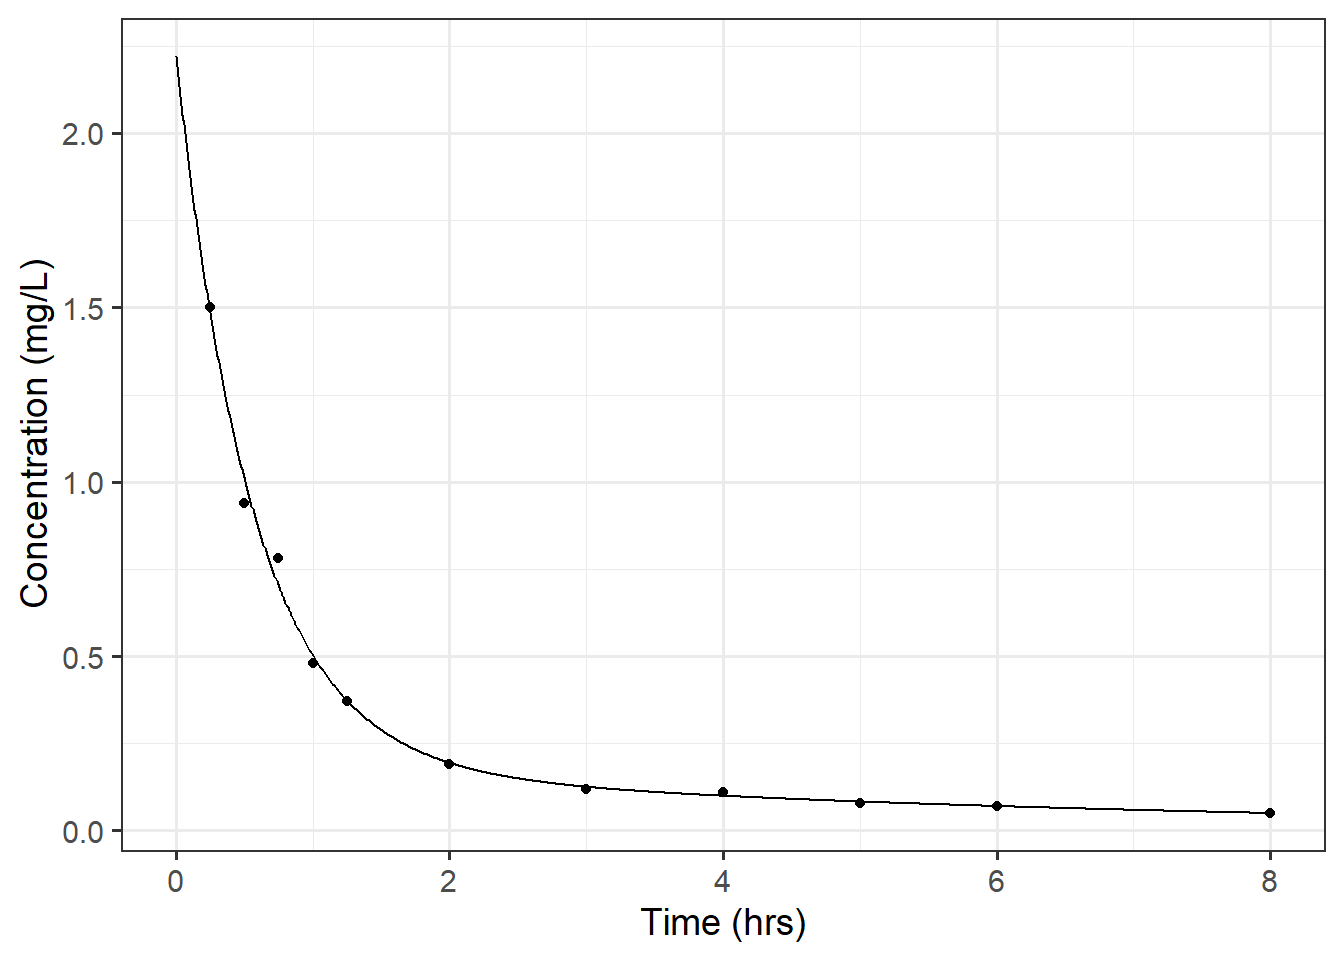
\includegraphics[width=0.8\textwidth]{./Images/nlm-indomethacin-plot-1} 

}

\caption{Concentration of Indomethacin in a single subject with the estimated nonlinear model overlayed.}\label{fig:nlm-indomethacin-plot}
\end{figure}

While not immediately obvious from the plot of the data, fitting the model and examining the residuals (Figure \ref{fig:nlm-indometh-resids}) reveals that while the bi-exponential model seems appropriate for the mean response function, it seems unreasonable to assume the variance of the response is constant.

\begin{figure}

{\centering 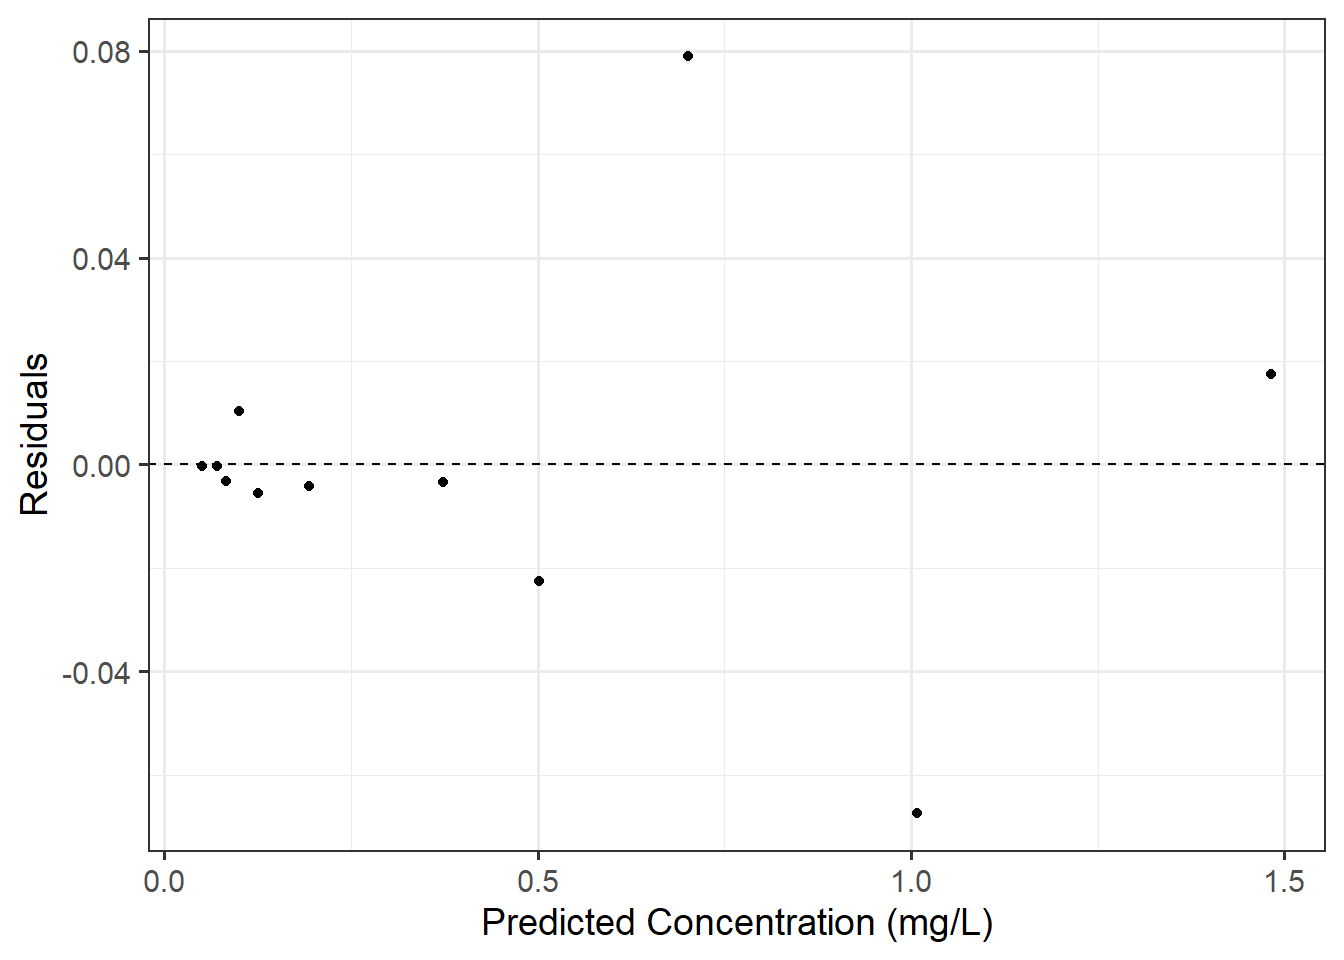
\includegraphics[width=0.8\textwidth]{./Images/nlm-indometh-resids-1} 

}

\caption{Plot of the residuals against predicted values for the Indomethacin example.}\label{fig:nlm-indometh-resids}
\end{figure}

Recall that violations of this condition does not mean our estimates are inappropriate. It means that our model for the sampling distribution will be inappropriate. As a result, confidence intervals and p-values produced will be invalid.

\hypertarget{modeling-the-variance}{%
\section{Modeling the Variance}\label{modeling-the-variance}}

Notice that to assess the condition of constant variance, we plot the residuals against the predicted values. This is not necessarily intuitive. In fact, the condition states that the variability of the response is constant for all values of the predictors; so, it may seem more reasonable to plot the residuals against each predictor. In fact, this is sometimes taught in other texts and routinely done by analysts, and there is nothing wrong with that approach. We advocate for plotting the residuals against the predicted values because it highlights a common phenomena - the variability of the response often depends on the \emph{value} of the response.

Figure \ref{fig:nlm-indometh-resids} illustrates that as the concentration increases, the variability in the concentration tends to increase as well. That is, we have much more precision when measuring small concentrations, and we have much less precision when measuring large concentrations. When we have some sense of how the variability behaves, especially as a function of the mean response, we can model that structure.

\begin{definition}[Generalized Least Squares]
The nonlinear modeling framework can be generalized to capture non-constant variance by altering the moment model. Specifically, we consider

\[
\begin{aligned}
  E\left[(\text{Response})_i \mid (\text{Predictors})_i\right]
    &= f\left((\text{Predictors})_i, \boldsymbol{\beta}\right) \\
  Var\left[(\text{Response})_i \mid (\text{Predictors})_i\right]
    &= g\left((\text{Predictors})_i, \boldsymbol{\beta}, \boldsymbol{\gamma}\right)
\end{aligned}
\]

Such a model is fit with the method of generalized least squares in which we alternate between minimizing the distance between the observed response and the mean function and the minimizing the distance between the squared residuals and the variance function.
\end{definition}

The generalized least squares approach extends ordinary least squares to account for non-constant variance. Essentially, it down-weights responses which have less precision when fitting the model. As an iterative process, it allows the parameters in the mean model to be updated based on the variance estimates and the estimates in the variance function to be updated based on the mean estimates. Further, allowing the variance function to depend on the parameters in the mean response function captures behaviors like that in the Indomethacin example in which the variability is dependent upon the values of the response. A popular model is the power of the mean model.

\begin{definition}[Power of the Mean Model]
Allows the variance to be specified as a power of the mean response function. Specifically, we consider

\[
\begin{aligned}
  E\left[(\text{Response})_i \mid (\text{Predictors})_i\right]
    &= f\left((\text{Predictors})_i, \boldsymbol{\beta}\right) \\
  Var\left[(\text{Response})_i \mid (\text{Predictors})_i\right]
    &= \sigma^2 \left[f\left((\text{Predictors})_i, \boldsymbol{\beta}\right)\right]^{2\theta}
\end{aligned}
\]
\end{definition}

The implementation of generalized least squares is beyond the scope of this text. We simply mention that this is a method for addressing non-constant variance, and that once implemented, results in appropriate inference about the parameters in the mean model.

\hypertarget{wild-bootstrap}{%
\section{Wild Bootstrap}\label{wild-bootstrap}}

In Chapter \ref{glm-large-sample-theory}, we introduced the residual bootstrap as a method of relaxing distributional conditions. Specifically, the residual bootstrap avoided the need to assume the errors in a linear model followed a Normal distribution. However, it still required assuming the variability of the errors was constant. In this section, we extend these ideas to overcome heteroskedasticity in nonlinear models.

At first glance, it is not obvious why an additional algorithm for bootstrapping is necessary. In addition to the residual bootstrap, we discussed case-resampling as a method of bootstrapping. This method does not require that we assume the variability of the response is constant for all values of the predictor. However, the performance of this particular algorithm can be quite poor in nonlinear settings due to the lower sample sizes that are common. In particular, fitting a nonlinear model can be very unstable. If we do not observe data in key regions that define the curvature, the numerical algorithms underlying the minimization can fail to converge to a solution. As an example, consider the Indomethacin data in Figure \ref{fig:nlm-indomethacin-plot}. Suppose that we performed a single bootstrap resample in which we resampled \(n = 11\) observations, with resampling, at random. It is quite possible that we end up with a resample containing only data between times 2 and 8 only missing the most prominent curvature in the data. As a result, attempting to fit the bi-exponential model to the resample will fail. This is not the result of specific software limitations; this is a failure to have enough data to adequately model the structure.

So, case-resampling avoids assuming constant variance but can fail spectacularly in some nonlinear models. The residual bootstrap, on the other hand, assumes constant variance. It does, however, maintain the curvature as the same predictor values are used when performing each resample. Instead, pseudo-responses are generated in each bootstrap resample by adding a sample of the residuals to the fitted values (``jittering'' the fitted line). The wild bootstrap is an alteration of the residual bootstrap which relaxes the assumption of constant variance while maintaining this beneficial property of the residual bootstrap.

\begin{definition}[Wild Bootstrap]
Suppose we observe a sample of size \(n\) and use it to fit the mean model (linear or nonlinear)

\[E\left[(\text{Response})_i \mid (\text{Predictors})_i\right]= f\left((\text{Predictors})_i, \boldsymbol{\beta}\right)\]

to obtain the ordinary least squares estimates \(\widehat{\boldsymbol{\beta}}\). The wild bootstrap proceeds along the following algorithm:

\begin{enumerate}
\def\labelenumi{\arabic{enumi}.}
\tightlist
\item
  Compute the residuals
  \[(\text{Residual})_i = (\text{Response})_i - (\text{Predicted Response})_i\]
\item
  Construct new pseudo-residuals by multiplying each residual by a random variable \(U\) such that \(E\left(U_i\right) = 0\) and \(Var\left(U_i\right) = 1\), for example \(U_i \sim N(0,1)\):
  \[(\text{Pseudo-Residual})_i = U_i (\text{Residual})_i\]
\item
  Form ``new'' responses \(y_1^*, \dotsc, y_n^*\) according to
  \[y_i^* = (\text{Predicted Response})_i + (\text{Pseudo-Residual})_i.\]
\item
  Obtain the least squares estimates \(\widehat{\boldsymbol{\alpha}}\) by finding the values of \(\boldsymbol{\alpha}\) which minimize
  \[\sum_{i=1}^{n} \left(y_i^* - f\left((\text{Predictors})_i, \boldsymbol{\alpha}\right)\right)^2.\]
\item
  Repeat steps 2-4 \(m\) times.
\end{enumerate}

We often take \(m\) to be large (at least 1000). After each pass through the algorithm, we retain the least squares estimates from the resample. The distribution of the estimates across these resamples is a good empirical model for the sampling distribution of the original least squares estimates.
\end{definition}

The wild bootstrap alters the residuals (as opposed to resampling them as in the residual bootstrap) to mimic the variability of the response being potentially unique for each observation. The theoretical underpinnings are beyond the scope of this text, but intuitively, we are adding noise to the line (``jittering'' the predicted model) such that the noise has mean zero (meaning the model is still correctly specified) and has variance of the same magnitude as the original observation (captured by the magnitude of the residual).

This process is computationally intensive but can dramatically improve inference when necessary.

\hypertarget{nlm-logistic}{%
\chapter{Logistic Regression}\label{nlm-logistic}}

When the response is binary (taking one of only two values), the models we have discussed so far in this text are inappropriate. To see some of the complications, consider trying to characterize the impact of lifestyle choices on whether an individual is diagnosed with cancer. The response (is a person diagnosed with cancer, yes/no) does not readily fit into a framework such as

\[(\text{Response})_i = f\left((\text{Predictors})_i, \boldsymbol{\beta}\right) + \varepsilon_i.\]

To begin with, the left-hand side is not a number, but a categorical variable. We could potentially address this using an indicator variable:

\[(\text{Cancer Diagnosis})_i = \begin{cases} 1 & \text{if i-th subject diagnosed with cancer} \\ 0 & \text{otherwise} \end{cases};\]

we could use this indicator variable as the response. However, we now have another issue; the right-hand side of the model would need to only return either a 0 or a 1. The response will \emph{never} be 0.96; as a result, the idea of \(\varepsilon_i\) being errors that ``jitter'' the observed response from some overall mean response is no longer reasonable.

The nonlinear model framework is general enough to permit binary responses. Specifically, when the response is binary, the most common technique is logistic regression, which is the focus of this chapter. Many other texts consider logistic regression to be a separate topic; however, as the structure is nonlinear in the parameters, we present it in this unit as a way of bringing together many of the ideas we have discussed within the context of nonlinear models.

\hypertarget{considerations-for-a-binary-response}{%
\section{Considerations for a Binary Response}\label{considerations-for-a-binary-response}}

The benefit of the nonlinear model framework we outlined in Chapter \ref{nlm-framework} is that it emphasizes that regression models simply characterize aspects of the distribution of the response. When the response is binary, we know quite a bit about the distribution.

Chapter \ref{essential-probability} introduced common models for the distribution of a random variable. When the random variable is quantitative, there are many potential distributional models. However, when the response is binary, there is only a single model for characterizing the distribution: the Bernoulli distribution (Definition \ref{def:defn-bernoulli-distribution}). Therefore, we can leverage that in developing a model for a binary response.

In particular, the Bernoulli distribution states that the mean response \(p\) is a value between 0 and 1 representing the probability the response takes the value 1 (representing a ``success''). Further, the variance of the response is determined by the mean response \((p (1 - p))\). Of course, the definition of the Bernoulli distribution considers the parameter \(p\) to be a single value. As we have seen, regression models allow the distribution to depend on additional predictors.

Placing this in the nonlinear model framework, we would say

\[
\begin{aligned}
  E\left[(\text{Response})_i \mid (\text{Predictors})_i\right] 
    &= f\left((\text{Predictors})_i, \boldsymbol{\beta}\right) \\
  Var\left[(\text{Response})_i \mid (\text{Predictors})_i\right]
    &= f\left((\text{Predictors})_i, \boldsymbol{\beta}\right) \left(1 - f\left((\text{Predictors})_i, \boldsymbol{\beta}\right)\right).
\end{aligned}
\]

The mean response function \(f(\cdot)\) is allowing the mean response (\(p\) in the Bernoulli distribution) to depend upon predictors. And, once the mean response function is specified, the variance is known (through the relationship \(p (1 - p)\)). However, since we know that the response is binary, we can go further and say not only is this an appropriate mean and variance function, but we know the distribution as well:

\[(\text{Response})_i \mid (\text{Predictors})_i \stackrel{\text{Ind}}{\sim}Ber\left[f\left((\text{Predictors})_i, \boldsymbol{\beta}\right)\right]\]

where we are assuming that each response is independent of all others. Remember, nothing about the nonlinear modeling framework prohibited making distributional assumptions; we just often were unwilling to. Here, we know the distribution; so, we include it as part of the model.

Of course, the nature of the binary response impacts our choice of the mean response function \(f(\cdot)\). In particular, the Bernoulli distributional model tells us that the mean response represents the probability the response takes the value 1. In our working example, this would be the probability of a subject receiving a cancer diagnosis given the values of the predictors. And, we know that probabilities must be between 0 and 1. Therefore, we must choose a mean response function \(f(\cdot)\) which has a range of 0 to 1.

This last point is what prohibits using linear regression with a binary response. The mean response function should represent a probability, but it is entirely likely that linear regression will result in probabilities less than 0 or larger than 1. Therefore, any reasonable choice of \(f(\cdot)\) will be nonlinear in the parameters.

While technically any function \(f(\cdot)\) which has a range on 0 to 1 is possible, one choice has dominated the literature in applied sciences for many years.

\hypertarget{the-logistic-regression-model}{%
\section{The Logistic Regression Model}\label{the-logistic-regression-model}}

If we want a large class of functions \(f(\cdot)\) which have a range on 0 to 1, we need only look to any cumulative distribution function (Definition \ref{def:defn-cdf}). The most popular choice is the cumulative distribution function of the Logistic distribution:

\[f(x) = \frac{e^x}{1 + e^x}.\]

This leads to the logistic regression model.

\begin{definition}[Logistic Regression Model]
A model for binary responses where the response, given the predictors, has a Bernoulli distribution such that

\[Pr\left((\text{Response})_i = 1 \mid (\text{Predictors})_i\right) = 
    \frac{e^{\beta_0 + \sum_{j=1}^{p} \beta_j (\text{Predictor } j)_i}}{1 + e^{\beta_0 + \sum_{j=1}^{p} \beta_j (\text{Predictor } j)_i}}\]

and all responses are independent of one another.
\end{definition}

While it is common in practice to consider the exponents to be linear combinations of the parameters, this is not technically a requirement. However, given our ability to capture curvature through flexible modeling techniques like splines, it is rare to see the exponent not be linear in the parameters.

\begin{rmdwarning}
Do not be fooled by the linear combination of the parameters in the exponent. The logistic regression model is nonlinear in the parameters since they occur in the exponent.\\
\end{rmdwarning}

As stated above, by specifying the above mean response function, we have also specified the variance of the response. It will have the form

\[\left(\frac{e^{\beta_0 + \sum_{j=1}^{p} \beta_j (\text{Predictor } j)_i}}{1 + e^{\beta_0 + \sum_{j=1}^{p} \beta_j (\text{Predictor } j)_i}}\right)\left(1 - \frac{e^{\beta_0 + \sum_{j=1}^{p} \beta_j (\text{Predictor } j)_i}}{1 + e^{\beta_0 + \sum_{j=1}^{p} \beta_j (\text{Predictor } j)_i}}\right).\]

We point this out to emphasize that the variance is not constant! Instead of addressing the non-constant variance through the wild bootstrap, we instead are modeling the structure of the variance directly.

\begin{rmdtip}
While not presented this way, it is possible to envision a binary response as the result of a latent quantitative response. For example, whether a student ``graduates with honors'' is a binary response (they either do or do not); but, it is the result of discretizing a quantitative measure (the student's GPA). Thinking of the observed binary response as a discretation of some \emph{unobserved} quantitative measure, with proper assumptions on the error term, will result in the above logistic regression model.
\end{rmdtip}

\hypertarget{estimation-of-the-parameters}{%
\section{Estimation of the Parameters}\label{estimation-of-the-parameters}}

The logistic regression model not only specifies the form of the mean and variance of the response; it also specifies the distributional model. As a result, we could specify the density function of the response given the predictors. Proceeding by estimating the parameters using least squares (as advocated in Chapter \ref{nlm-framework}) would actually ignore this additional information. When a parametric model is specified, we should take advantage of the additional structure (knowing the form of the density function) when estimating the parameters. This is accomplished through likelihood-theory.

While a full development of likelihood theory is beyond the scope of this text, we motivate its use. In a probability course, the density function of a random variable is fully known, and we use it to compute the probability of the random variable taking on specific values. In a statistics course, we work in reverse. We have already observed specific outcomes; but, the density function is not fully known (as the parameters are unknown). We want to choose values of the unknown parameters that would result in a density function making the observed data as likely as possible.

Consider a specific example. Suppose we \emph{spin} a penny 100 times and observe it landing ``tails-side up'' in 82 of those trials. If you had to guess at the true probability of a penny landing ``tails-side up'' when spun, what would you guess based on this data? Putting it into our logistic model framework, consider the indicator

\[
(\text{Tails})_i = \begin{cases} 1 & \text{if i-th spin lands tails-side up} \\ 0 & \text{otherwise} \end{cases};
\]

then, our logistic model (with no predictors) has the form

\[Pr\left((\text{Tails})_i = 1\right) = \frac{e^{\beta_0}}{1 + e^{\beta_0}}.\]

We want to choose a value of \(\beta_0\) which makes it as likely as possible (maximizes the probability) that in a new sample of 100 spun pennies, 82 would land tails-side up. Why do we make this as likely as possible? Because that is the data that we observed and is the only information we have on this process. Therefore, we want a model that aligns with this data as closely as possible, or more accurately, we want the data to align with the model as closely as possible. Hopefully, it is intuitive that if \emph{in reality}, a penny lands ``tails-side up'' 82\% of the time, that makes this observed data much more likely than if \emph{in reality}, it lands ``tails-side up'' only 50\% of the time. Therefore, we would want the above probability to be equal to 0.82, leading to an estimate of \(\beta_0\).

To help with visualizing this process, Figure \ref{fig:nlm-coins-likelihood} gives the probability of observing 82 coins (out of a sample of 100) land ``tails-side up'' as the value of \(\beta_0\) changes. The likelihood is maximized when we set the true value of a ``tails-side up'' at being 0.82 (corresponding to \(\beta_0 = 1.516\)). Other values can make the data likely, but not as likely as that value.

\begin{figure}

{\centering 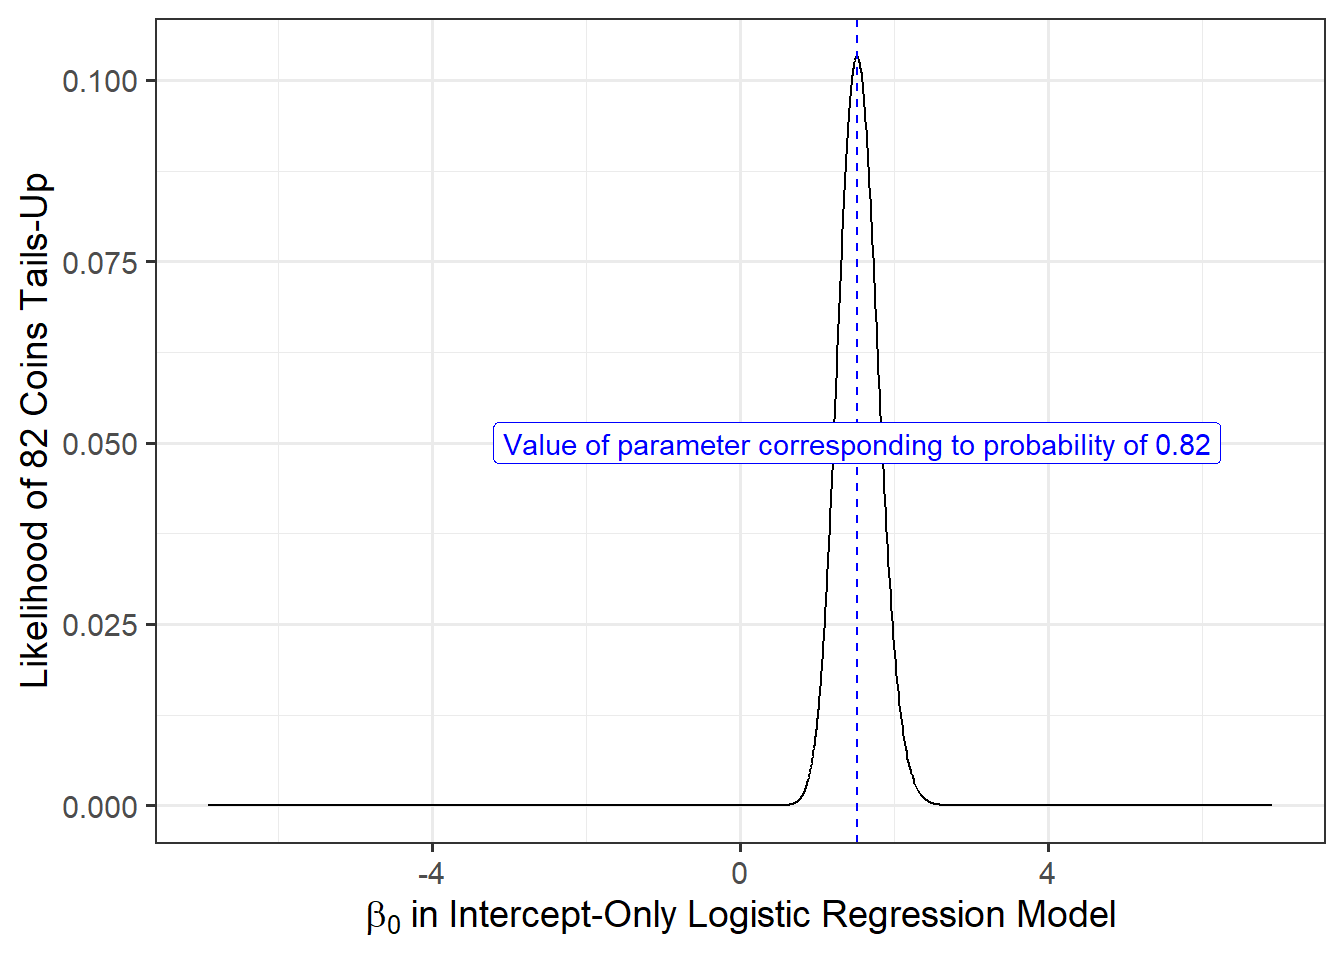
\includegraphics[width=0.8\textwidth]{./Images/nlm-coins-likelihood-1} 

}

\caption{Likelihood of observing 82 coins land tails-side up when spinning 100 independent pennies. The likelihood is over possible values of the parameter governing an intercept-only logistic regression model.}\label{fig:nlm-coins-likelihood}
\end{figure}

We generalize this to saying that for a fully parametric nonlinear model (such as logistic regression), it is best to choose the values of the parameters that maximize the likelihood function.

\begin{definition}[Likelihood Function]
For a fully parametric model, the likelihood function \(\mathcal{L}(\boldsymbol{\beta}, \text{Observed Data})\) captures how likely the observed data is to be realized in a future study under a specific set of parameters. This is directly related to the density function of the parametric model assumed.
\end{definition}

\begin{definition}[Maximum Likelihood Estimation]
Choosing parameter estimates to maximize the likelihood function under an assumed parametric model. The resulting estimates are known as maximum likelihood estimates.
\end{definition}

While the actual form is not critical to our exposition, for completeness, we provide the likelihood function corresponding to logistic regression:

\[\prod_{i=1}^{n} \left(\frac{e^{\beta_0 + \sum_{j=1}^{p} \beta_j (\text{Predictor } j)_i}}{1 + e^{\beta_0 + \sum_{j=1}^{p} \beta_j (\text{Predictor } j)_i}}\right)^{(\text{Response})_i}\left(1 - \frac{e^{\beta_0 + \sum_{j=1}^{p} \beta_j (\text{Predictor } j)_i}}{1 + e^{\beta_0 + \sum_{j=1}^{p} \beta_j (\text{Predictor } j)_i}}\right)^{1 - (\text{Response})_i}\]

where \((\text{Response})_i\) is an indicator value taking the value 1 or 0. Maximizing this likelihood is done numerically. While the details of this process are beyond the scope of this text, the procedure is similar to the least-squares procedure discussed in Chapter \ref{nlm-estimation}.

\hypertarget{inference-on-the-parameters-1}{%
\section{Inference on the Parameters}\label{inference-on-the-parameters-1}}

In order to make inference about the parameters, we need a model for the sampling distribution of the parameter estimates. Likelihood-theory provides results for modeling the sampling distribution of maximum likelihood estimates. Generally, these results rely on large-sample theory (though empirical models could be developed).

\begin{definition}[Large Sample Sampling Distribution of Parameter Estimates in Logistic Regression Models]
Assuming the form of the model is correctly specified with parameter vector \(\boldsymbol{\beta}\), as the sample size gets large, we have that

\[\frac{\widehat{\beta}_j - \beta_j}{\sqrt{Var\left(\widehat{\beta}_j\right)}} \sim N(0, 1)\]

for all \(j = 1, \dotsc, p\). Further, under the null hypothesis

\[H_0: \mathbf{K}\boldsymbol{\beta} = \mathbf{m}\]

we have

\[\left(\mathbf{K}\widehat{\boldsymbol{\beta}} - \mathbf{m}\right)^\top \left(\mathbf{K}\widehat{\boldsymbol{\Sigma}}\mathbf{K}^\top\right)^{-1} \left(\mathbf{K}\widehat{\boldsymbol{\beta}} - \mathbf{m}\right) \sim \chi^2_r\]

where \(r\) is the rank (number of rows) of \(\mathbf{K}\).
\end{definition}

\begin{rmdtip}
Though the above results require large sample sizes, generally fitting a logistic regression model itself requires a relatively large sample size (the less variability in the response, the harder it is to fit a model). As a result, being able to estimate the parameters often means the sample size is large enough to rely on the default inference.
\end{rmdtip}

As stated in Chapter \ref{nlm-framework}, adding distributional assumptions does not avoid the need for large-sample inference. The difference is primarily in the estimation process (least squares compared to maximum likelihood). When we do know the distributional model (as in the case of logistic regression), it turns out maximum likelihood estimation is optimal.

\begin{rmdwarning}
When we have a binary response, we \emph{know} it has a Bernoulli distribution. As a result, we do not need to posit a model for the distribution. However, that does not guarantee our model is specified correctly in logistic regression because we may have misspecified the mean response function.
\end{rmdwarning}

The above results allow us to not only construct confidence intervals, but we can also make use of the general linear hypothesis testing framework for testing specific hypotheses. That is, our inference is not all that different than under the linear model framework once we have estimates for the parameters and estimates for their standard errors.

\hypertarget{interpretation-of-parameters}{%
\section{Interpretation of Parameters}\label{interpretation-of-parameters}}

The parameters in a logistic model have a nice interpretation; however, that interpretation is not a natural scale for most individuals. In order to understand what is happening, we need to think in terms of odds instead of probabilities.

\begin{definition}[Odds]
The odds of an event with probability \(p\) is defined as

\[\frac{p}{1-p}\]
\end{definition}

We often hear odds presented in terms of integers. Such as, ``there are 3-to-1 odds the event will occur.'' This would mean that out of four trials, we would expect the event to happen 3 times; this corresponds to \(p = 0.25\) and therefore \(1 - p = 0.75\) given an odds of 3. While many of us think in terms of probabilities, clinicians tend to think in terms of the odds of an event. As a result, it is natural to clinicians to compare the odds of an event under two scenarios instead of comparing the probability of an event under two scenarios.

\begin{definition}[Odds Ratio]
The odds ratio is a method of comparing two events; typically, it is formed by the ratio of the odds of the same event under two different scenarios. Let \(p_1\) be the probability of the event under scenario 1 and let \(p_2\) be the probability of an event under scenario 2; then, the odds of the event under scenario 1 are

\[\gamma_1 = \frac{p_1}{1 - p_1}\]

and the odds of the event under scenario 2 are

\[\gamma_2 = \frac{p_2}{1 - p_2}\]

and the odds ratio comparing scenario 1 to scenario 2 is

\[OR = \frac{\gamma_1}{\gamma_2} = \left(\frac{p_1}{1 - p_1}\right) \left(\frac{1 - p_2}{p_2}\right).\]
\end{definition}

If the odds of the event are the same under both scenarios, we obtain an odds ratio of 1. Odds ratios larger than 1 indicate that the event is more likely to occur (has greater odds) under scenario 1. Odds ratios less than 1 indicate that the event is less likely to occur (has lower odds) under scenario 1.

Now, let's return to our logistic regression model. Consider a model with two predictors:

\[Pr\left((\text{Response})_i = 1 \mid (\text{Predictors})_i \right) = \frac{\exp\left\{\beta_0 + \beta_1 (\text{Predictor 1})_i + \beta_2 (\text{Predictor 2})_i\right\}}{1 + \exp\left\{\beta_0 + \beta_1 (\text{Predictor 1})_i + \beta_2 (\text{Predictor 2})_i\right\}}.\]

Consider the group of subjects where Predictor 1 takes the value \(a\) and Predictor 2 takes the value \(b\). Then, the probability the response takes the value 1 in this group is

\[p_a = \frac{e^{\beta_0 + \beta_1 a + \beta_2 b}}{1 + e^{\beta_0 + \beta_1 a + \beta_2 b}}\]

and the odds of the response taking the value 1 are

\[\frac{p_a}{1 - p_a} = e^{\beta_0 + \beta_1 a + \beta_2 b}.\]

Now, consider the group of subjects where Predictor 1 takes the value \(a + 1\) and Predictor 2 takes the value \(b\). Then, following the above process, we have that the probability the response takes the value 1 in this group is

\[p_{a+1} = \frac{e^{\beta_0 + \beta_1 (a + 1) + \beta_2 b}}{1 + e^{\beta_0 + \beta_1 (a + 1)+ \beta_2 b}}\]

and the odds of the response taking the value 1 are

\[\frac{p_{a+1}}{1 - p_{a+1}} = e^{\beta_0 + \beta_1 (a + 1) + \beta_2 b}.\]

Now, the odds ratio for the group with an increase in Predictor 1 relative to the other group is

\[\left(\frac{p_{a+1}}{1 - p_{a+1}}\right) \left(\frac{1 - p_a}{p_a}\right) = e^{\beta_1}.\]

That is, the parameters in the logistic regression model are directly related to the odds ratio.

\begin{definition}[Interpretation of Parameters in Logistic Regression Model]
Let \(\beta_j\) be the parameter associated with the \(j\)-th predictor in the logistic regression model. Then, \(\beta_j\) represents the log-OR (``log odds ratio'') associated with a one-unit increase in the \(j\)-th predictor holding all other predictors fixed.
\end{definition}

That is, exponentiating the \(j\)-th coefficient gives the odds ratio comparing the odds of the event under two scenarios: when the \(j\)-th predictor is increased by 1 unit relative to leaving it alone. Notice that unlike the linear model, increasing the \(j\)-th predictor by 1 unit does not result in an additive effect on the mean response (the probability of the response occurring in this case). Instead, it has an additive effect on the log odds.

\begin{rmdtip}
When we use the word ``log'' throughout, we are referring to the natural logarithm.
\end{rmdtip}

As a result, if a parameter in our model is 0, it will result in an odds ratio of 1, indicating no association between the response and predictor. A parameter larger than 0 results in an odds ratio larger than 1, indicating that the likelihood of the response increases as the predictor increases. A parameter smaller than 0 results in an odds ratio less than 1, indicating the likelihood of the response decreases as the predictor increases.

\hypertarget{nlm-selection}{%
\chapter{Model Selection}\label{nlm-selection}}

As we have seen, hypothesis testing is really a formal way of comparing two models --- a simplified model and a more complex model. However, this form of model comparisons requires the simple model to be a subset of the more complex model (referred to as nested testing). We may be interested in comparing two competing (yet equally complex) models. In such cases, the general linear hypothesis testing framework does not work; so, we turn to likelihood-based model selection criteria.

There are several ways to quantify how well a model fits a set of data, or more accurately, how closely the data fits a particular model. The most well-known is R-squared.

\begin{definition}[R-squared]
The proportion of the variability in the response explained by the model. When the response is quantitative, R-squared is defined as

\[R^2 = \frac{SSR}{SST} = 1 - \frac{SSE}{SST} = 1 - \frac{\sum_{i=1}^{n} (\text{Residuals})_i^2}{\sum_{i=1}^{n} \left((\text{Response})_i - (\text{Average Response})\right)^2}.\]

When the response is categorical (such as logistic regression), there is no unique definition of R-squared.
\end{definition}

R-squared has a nice interpretation and is often used to quantify the quality of the model fit. However, it is not a great criteria for comparing models. It can be proven that R-squared will continue to increase as the model becomes more complex. In fact, in many situations it is possible to add enough terms that you will obtain an R-squared value of 1 indicating perfect fit (visually, think about connecting the dots). However, this is the result of overfitting.

\begin{definition}[Overfitting]
Constructing a model that accurately predicts the observed data at the expense of accurate variance estimation and model parsimony. As a result, the model will have poor prediction for future observations.
\end{definition}

Remember, models are never correct; by nature, they are simplifications of a complex process. We do, however, want our models to be useful. Creating a model that predicts well in the sample performs poorly outside the sample is not helpful, and it could lead to incorrectly characterizing the scientific behavior being observed. As a result, we want a different metric for assessing model performance when comparing models.

\begin{rmdtip}
There are a couple ``adjusted R-squared'' metrics which do take into account model complexity. We do not discuss them in this text as they tend to be reserved for linear models and it is not obvious how to generalize them to other model settings.
\end{rmdtip}

As introduced in Chapter \ref{nlm-logistic}, when we define a fully parametric model, we can use likelihood-theory to fit the model. In particular, the maximum likelihood estimates are the values of the parameters which maximize the likelihood function (Definition \ref{def:defn-likelihood}). Larger values of the likelihood (under an estimated model) indicate stronger agreement with the data. That is, larger values of the likelihood indicate a better fit. This suggests a general metric for assessing models regardless of their complexity known as information criteria.

\begin{definition}[Information Criteria]
Metrics which balance the model fit (through the likelihood function) with model complexity through some penalty term.
\end{definition}

Information criteria do not have an intuitive scale like R-squared; therefore, the value has no natural interpretation. However, they do allow for comparisons between arbitrary models.

\begin{rmdwarning}
Information criteria rely on the likelihood; as a result, they only truly make sense when we are willing to assume the parametric model is appropriate. The computer can always compute them, but we should understand that they assume some distributional model for the response.
\end{rmdwarning}

While there have been several information criteria proposed (and more continue to be developed), there are two which are very well known examples which are often defaults in software: AIC and BIC.

\begin{definition}[AIC]
Given a model \(\mathcal{M}\), Akaike's information criterion (AIC) is defined as

\[\text{AIC}_{\mathcal{M}} = -2\ln\left(\widehat{L}_{\mathcal{M}}\right) + 2p_{\mathcal{M}}\]

where \(\widehat{L}_{\mathcal{M}}\) represents the likelihood function corresponding to model \(\mathcal{M}\) when evaluated at the maximum likelihood estiamtes, and \(p_{\mathcal{M}}\) is the number of parameters in \(\mathcal{M}\).
\end{definition}

Larger values of the likelihood function indicate better agreement; similarly, we prefer parsimonious models when possible. Therefore, \emph{lower} values of AIC are preferred. It favors models which fit the data well (high likelihood) but penalizes for overly complex models (too many parameters). Of course, this penalty is the same regardless of the sample size. This inspires BIC.

\begin{definition}[BIC]
Given a model \(\mathcal{M}\), Schwarz's Bayesian information criterion (BIC) is defined as

\[\text{BIC}_{\mathcal{M}} = -2\ln\left(\widehat{L}_{\mathcal{M}}\right) + p_{\mathcal{M}} \ln(n).\]
\end{definition}

Note that the formula for BIC is nearly identical to that of AIC. As with AIC, lower values of BIC are preferred. With information criteria, as there is no natural scale, it only makes sense to compare models on the same set of data (you cannot compare the AIC from one study to the AIC of a different study). There is also no p-value for determining if the difference in AIC (or BIC) values for two models is ``significant.'' Lower is simply better; however, some people do advocate various rules of thumb. For our purpose, if the values between two models are at all close, it should be a subject-matter decision: which model better explains the scientific process? Alternatively, if it is close, choose the model that is easier to interpret.

\hypertarget{nlm-estimation}{%
\chapter{Estimation Details}\label{nlm-estimation}}

We have stated that numerical methods are needed to obtain estimates of the parameters for nonlinear models. Here we introduce the primary algorithm used for obtaining these estimates and sketch out some ideas for how this is implemented in practice. Readers may skip this section without loss of continuity.

When we begin working with nonlinear models, we will often come across computational issues. In order to begin diagnosing these issues, we must have some understanding of the underlying algorithm. Our objective is to find the values of the parameters \(\boldsymbol{\beta}\) such that the mean function is close to the observed response. One way of defining close is to consider minimizing the sum of squared residuals. That is, we desire the values of \(\boldsymbol{\beta}\) that minimize

\[\sum_{i=1}^{n} \left((\text{Response})_i - f\left((\text{Predictors})_i, \boldsymbol{\beta}\right)\right)^2.\]

We called the value that minimizes this objective function the ordinary least squares estimates.

\begin{rmdwarning}
This chapter applies to ordinary least squares. Logistic regression, which makes use of maximum likelihood estimation has a slightly different objective function.\\
\end{rmdwarning}

For the remainder of this chapter, let \(y_i\) denote the response and \(\mathbf{x}_i\) the vector of predictors for the \(i\)-th observation. Then, minimizing the objective function above is equivalent to finding the values of \(\boldsymbol{\beta}\) which solves the system of equations given by

\[\sum_{i=1}^{n} \left(y_i - f\left(\mathbf{x}_i, \boldsymbol{\beta}\right)\right) f_{\boldsymbol{\beta}}\left(\mathbf{x}_i, \boldsymbol{\beta}\right)\]

where \(f_{\boldsymbol{\beta}}\) represents the gradient vector (with respect to the parameters) of the mean function \(f\). Solving this system of equations is our primary objective. This is typically done via the Gauss-Newton Method.

\begin{definition}[Gauss-Newton Method]
The most commonly used optimization routine for statistical applications, this method relies on linearizing the problem using a Taylor Series approximation.
\end{definition}

Observe that for a value \(\boldsymbol{\beta}^*\) close to \(\boldsymbol{\beta}\), a Taylor Series approximation gives

\[
\begin{aligned}
  f\left(\mathbf{x}_i,\boldsymbol{\beta}\right)
    &\approx f\left(\mathbf{x}_i,\boldsymbol{\beta}^*\right) + f^\top_{\boldsymbol{\beta}}\left(\mathbf{x}_i,\boldsymbol{\beta}^*\right)\left(\boldsymbol{\beta} - \boldsymbol{\beta}^*\right) \\
  f_{\boldsymbol{\beta}}\left(\mathbf{x}_i,\boldsymbol{\beta}\right)
    &\approx f_{\boldsymbol{\beta}}\left(\mathbf{x}_i,\boldsymbol{\beta}^*\right) + f_{\boldsymbol{\beta}\boldsymbol{\beta}}\left(\mathbf{x}_i,\boldsymbol{\beta}^*\right)\left(\boldsymbol{\beta} - \boldsymbol{\beta}^*\right)
\end{aligned}
\]

where \(f_{\boldsymbol{\beta}\boldsymbol{\beta}}\) is a \(p\)-by-\(p\) matrix of second partial derivatives. We appeal to a linear approximation because if \(\boldsymbol{\beta}^*\) is sufficiently close to \(\boldsymbol{\beta}\), then higher order terms are negligible.

Now, we substitute these approximations into the system of equations we need to solve. We end up with four terms, of which the last is small because it has quadratic terms, and the third is small because on average, we expect \(y_i - f(\mathbf{x}_i,\boldsymbol{\beta}^*)\) to be small, which when multiplied by \((\boldsymbol{\beta} - \boldsymbol{\beta}^*)\) is really small. Thus, we are left with the approximation

\[
  \sum\limits_{i=1}^{n} f_{\boldsymbol{\beta}}\left(\mathbf{x}_i,\boldsymbol{\beta}^*\right)f_{\boldsymbol{\beta}}^\top\left(\mathbf{x}_i,\boldsymbol{\beta}^*\right)\left(\boldsymbol{\beta}-\boldsymbol{\beta}^*\right) = \sum\limits_{i=1}^{n} \left(y_i - f(\mathbf{x}_i,\boldsymbol{\beta}^*)\right)f_{\boldsymbol{\beta}}(\mathbf{x}_i,\boldsymbol{\beta}).
\]

We solve this for \(\boldsymbol{\beta}\) to obtain an iterative scheme for updating estimates of \(\boldsymbol{\beta}\) given a current estimate. That is, given initial estimates \(\boldsymbol{\beta}^{(0)}\), we perform iterative updates, terminating the algorithm when two successive iterations yield estimates which are close (iterations converged).

One of the key lessons here is that starting estimates of the parameters are always needed, as we have seen in our previous examples. This is always a case when numerical methods are used. There are no all-encompassing strategies here; determining starting values is unique to each problem. Often times, starting values can be obtained by making large simplifications or transformations to the model to get a rough idea of the estimates.

As an example, consider the Michaelis-Menten model:

\[E\left((\text{Response})_i \mid (\text{Predictor})_i\right) = f\left((\text{Predictor})_i, \boldsymbol{\theta}\right) = \frac{\theta_1 (\text{Predictor})_i}{\theta_2 + (\text{Predictor})_i}.\]

In this model, \(\theta_1\) represents the maximum possible response and \(\theta_2\) the shape parameter known as the inverse affinity. Starting values for this model are obtained by considering a transformation. Specifically observe that if we take the inverse of the observed response, we have

\[\frac{1}{E\left((\text{Response})_i \mid (\text{Predictor})_i\right)} = \frac{\theta_2 + (\text{Predictor})_i}{\theta_1 (\text{Predictor})_i} = \frac{\theta_2}{\theta_1} \left(\frac{1}{(\text{Predictor})_i}\right) + \frac{1}{\theta_1}.\]

This motivates considering a linear model of the form

\[(\text{Inverse Response})_i = \beta_0 + \beta_1 (\text{Inverse Predictor})_i + \varepsilon_i.\]

The estimate of \(\beta_0\) will allow us to compute an estimate for \(\theta_1\) where

\[\widehat{\theta}_1 = \frac{1}{\widehat{\beta}_0}\]

and the estimate of \(\beta_1\) will allow us to compute an estimate for \(\theta_2\) where

\[\widehat{\theta}_2 = \widehat{\beta}_1 \widehat{\theta}_1.\]

We now have starting estimates that would allow us to resume fitting the nonlinear model on the original scale.

\hypertarget{nlm-rm}{%
\chapter{Nonlinear Models with Repeated Measures}\label{nlm-rm}}

Just as the linear model could be extended to account for repeated measures, nonlinear models can be extended as well. This is most commonly done through the mixed models framework. As with the previous chapter, we provide some guidance for extending the nonlinear modeling framework for those interested. Readers may skip this chapter without loss of continuity.

Recall the Theophylline example (\ref{exm:nlm-theoph}) we used to introduce nonlinear models at the beginning of this unit. Researchers were interested in studying the pharmacokinetics of the antiasthmatic agent. In the original example, we considered blood samples taken from a single individual over a 24-hour period. In reality, the study enrolled 12 subjects, and each had blood samples taken over a 24-hour period. The goal of the study, and the goal of most pharmacokinetic studies, is to understand the way the body processes the drug \emph{across the population}. That is, researchers were interested in how the concentration-time profiles (through their parameters) varied across individuals. Since we have multiple measurements for each of the 12 subjects, we have repeated measures data.

Notice that the goal here is not to model the average trend in the population but to characterize the average (and even the variability) of in the parameters across individuals in the population. This is not the same as a confidence interval for the parameter (which would still be describing the average value); researchers want to know how different the parameters can be across individuals. This is the perfect set-up for a subject-specific modeling approach to the repeated measures.

Recall that within a subject, researchers believe the one-compartment model with first-order absorption is an appropriate scientific model. Therefore, our subject-level model has the form

\[(\text{Concentration})_{i,j} = \frac{k_{a,i} D_i}{\left(\beta_i/k_{e,i}\right)\left(k_{a,i} - k_{e,i}\right)} \left(e^{-k_{e,i} t_{i,j}} - e^{-k_{a,i} t_{i,j}}\right) + \varepsilon_{i,j},\]

where the parameters retain the same interpretations they had previously. While the form is held the same across all subjects, the specific values of the parameters can vary from one subject to another. The population-level model \emph{could} have the form

\[
\begin{aligned}
  k_{a,i} &= k_{a} + b_{1,i} \\
  k_{e,i} &= k_{e} + b_{2,i} \\
  \beta_i &= \beta + b_{3,i}
\end{aligned}
\]

where we assume each \(b_{k,i} \stackrel{\text{IID}}{\sim}N\left(0, \sigma^2_k\right)\) for each \(k\) and all are independent. That is, we are allowing each parameter to have a random effect which allows them to vary across the population. The parameter \(k_a\), for example, represents the average absorption rate across the population and \(\sigma_1^2\) would capture the variability of the absorption rate across the population. We could generalize the population-level model further to allow these parameters to depend upon other predictors (such as the weight of the subject).

These models are commonly fit (using specialized statistical software), but they continue to be the focus of research as there is not complete agreement on modeling constraints and how to relax conditions placed on the model. Unlike the linear case, it is not easy to determine the overall average trend given the subject-level model (though it is theoretically feasible). The nonlinearity makes several aspects of this problem quite challenging.

\hypertarget{part-survival-analysis}{%
\part{Survival Analysis}\label{part-survival-analysis}}

\hypertarget{surv-terminology}{%
\chapter{Key Terminolgy}\label{surv-terminology}}

Survival analysis (often referred to as ``reliability analysis'' in engineering) refers to the statistical analysis of studies for which the response is the time until an event occurs, such as the time until a device fails or the time until a subject dies. Studies involving such an endpoint often involve censoring --- the event of interest is not observed for every subject during the study period. In such situations, we must develop special models in order to obtain proper inference.

Models for survival analysis, in contrary to other models discussed in this text, are not generally concerned with the average response. Instead, they rely on different characterizations of the distribution of the response. While Chapter \ref{essential-probability} introduced basic methods for characterizing the distribution of a random variable, we need to extend these ideas in order to discuss survival analysis.

Let \(T\) represent the time until an event occurs; as we cannot predict this time with certainty, \(T\) is a random variable. Since it is a time, it could take on any value larger than 0; and, its distribution can be characterized through the probability density function \(f(t)\) (Definition \ref{def:defn-density}), which links the values it can assume with their likelihood.

\begin{example}[Carcinogen Exposure]
Consider a study in which rats were exposed to a carcinogen and then monitored closely. Suppose the distribution of the time \(T\) (in days) between exposure and the development of a tumor can be modeled with the following probability density function:

\[f(t) = \frac{1}{10} e^{-t/10} \qquad t > 0.\]
\end{example}

Survival analysis concerns itself primarily with the likelihood of remaining ``event-free.'' For example, for the Carcinogen Example, we might be interested in the proportion of rats that are still tumor free through 7 days; this translates to computing

\[Pr(T > 7) = \int_{7}^{\infty} f(t) dt.\]

Notice that this is the complement of the cumulative distribution function (CDF); it is known as the survival function.

\begin{definition}[Survival Function]
Let \(T\) be a random variable; the survival function \(S(u)\) is defined as

\[S(u) = Pr(T > u) = 1 - F(u),\]

capturing the probability of failing \emph{after} a time, where \(F(u)\) is the CDF of \(T\).

For a continuous random variable, we have that

\[S(u) = \int_{u}^{\infty} f(t) dt\]

implying that \(f(t) = -\frac{d}{dt} S(t)\).
\end{definition}

It should be clear from the definition that survival functions range between 0 and 1, and must have \(S(0) = 1\) and diminish towards 0 as time increases. In our example, this translates to rats being alive at the start of the study and all rats will die at some point after exposure.

In addition to the likelihood of being event-free past some point, we may want to know the likelihood of experiencing the event in the next unit of time \emph{given} the subject has been event-free up to that point. For example, what proportion of rats in the Carcinogen Example will develop a tumor within the next day \emph{given} the rats were tumor-free through seven days? The additional information (following ``given'') changes the computation; we are not interested in \(Pr(7 < T \leq 8)\) because the additional information says we are only interested in the subset of rats which are tumor-free through 7 days. We express this as \(Pr(T \leq 8 \mid T > 7)\). Since we are only interested in a subset of rats, we need to rescale (see Figure \ref{fig:surv-conditional-probability}):

\[Pr(T \leq 8 \mid T > 7) = \frac{Pr(7 < T \leq 8)}{Pr(T > 7)} = 1 - \frac{S(8)}{S(7)}.\]

\begin{figure}

{\centering 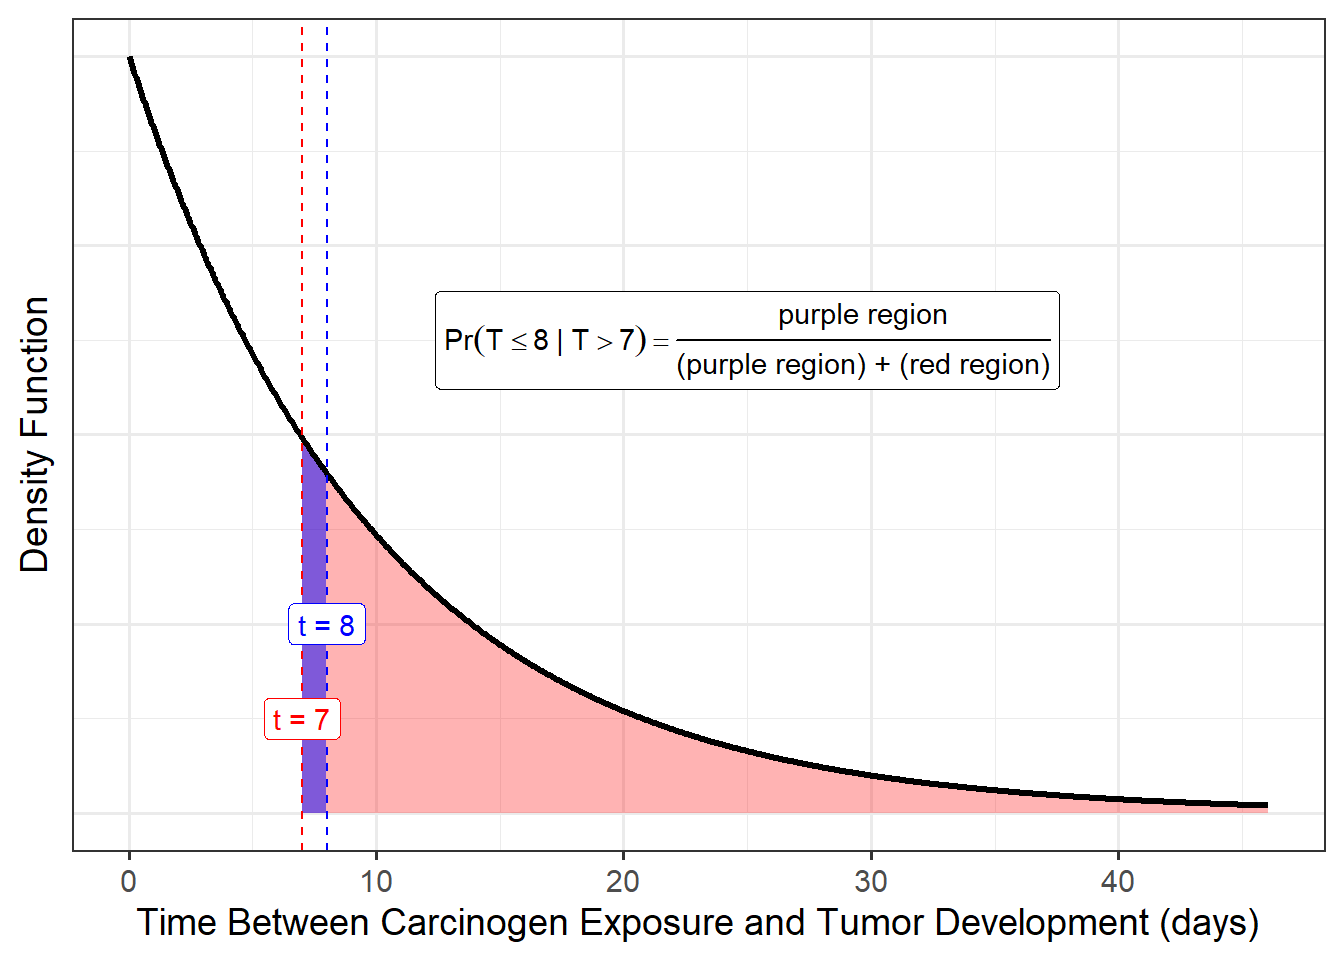
\includegraphics[width=0.8\textwidth]{./Images/surv-conditional-probability-1} 

}

\caption{Illustration of conditional probability.}\label{fig:surv-conditional-probability}
\end{figure}

This captures the event rate in the next time interval among survivors; this is known as the mortality rate.

\begin{definition}[Mortality Rate]
For any particular time \(t\), the morality rate \(m(t)\) is the proportion of the population who experience the event between times \(t\) and \(t + 1\), among individuals who are event-free at time \(t\). That is,

\[m(t) = Pr(t \leq T \leq t + 1 \mid T > t) = 1 - \frac{S(t + 1)}{S(t)}.\]
\end{definition}

The mortality rate considers a step of a single unit of time. Imagine taking a step of size \(h\), considering the proportion of deaths \emph{per unit time} with this step size, and then allowing this step size to become very small (mathematically, taking a limit). This would describe the instantaneous mortality rate, known as the hazard function.

\begin{definition}[Hazard Function]
For any time \(t\), the hazard function \(\lambda(t)\) is the instantaneous mortality rate per unit time:

\[\lambda(t) = \lim_{h \rightarrow 0} \frac{Pr(t \leq T \leq t + h \mid T > t)}{h} = \frac{f(t)}{S(t)} = -  \frac{\frac{d}{dt} S(t)}{S(t)} = -\frac{d}{dt} \log(S(t)).\]
\end{definition}

\begin{rmdwarning}
While the hazard function is related to probabilities, it is \emph{not} a probability. As a result, it can take on values much larger than 1.\\
\end{rmdwarning}

Larger values of the hazard function indicate a higher likelihood of the event. Given that each of these quantities is related to the density function, they are not technically necessary. However, as we will see, it turns out that it is sometimes easier to model on the hazard scale than modeling the density function. What is important to see is that if we are able to characterize the hazard function, we have also characterized the survival function and therefore the entire distribution (and vice versa).

The last component of the above definition emphasizes the relationship between the survival function and the hazard function. Inverting this relationship provides another quantity often referenced in survival analysis.

\begin{definition}[Cumulative Hazard]
For any time \(t\), we have that

\[S(t) = e^{-\int_{0}^{t} \lambda(u) du}\]

where

\[\Lambda(t) = -\int_{0}^{t} \lambda(u) du\]

is known as the cumulative hazard function.
\end{definition}

There are many named probability models used to characterize the distribution of an event time (Exponential, Gamma, Weibull, etc.). There are a few commonalities; each is defined over non-negative values as they are modeling the time until and event. Second, each tends to be right-skewed (the distribution has a ``slide'' shape with a long tail toward higher values). This is why it is often more common to report the median survival time instead of the average survival time as the average may be a misleading estimate of the center of the distribution. Such parametric models are quite common in engineering disciplines but are not as popular among the biological sciences, which tends to prefer a semiparametric approach.

\hypertarget{surv-censoring}{%
\chapter{Censoring}\label{surv-censoring}}

In an ideal world, survival analysis would be a standard analysis with a continuous response (time to event). The problem is that we often do not observe the response on a subject prior to the end of the study but instead only have partial information on the response; this phenomena, known as censoring, requires additional considerations. Consider the following example.

\begin{example}[Hypertension]
A study was conducted to examine the efficacy of a new anti-hypertensive medication. A cohort of 146 patients with previous history of heart disease were treated and then followed over the next 10 years. The primary event of interest was death, which was grouped into one year intervals.
\end{example}

As you might imagine, following patients over the span of years can be challenging. Occasionally, subjects are ``lost to follow-up.'' This can happen for a number of reasons. It could be that the subjects withdrew their consent for the study, prohibiting researchers from further contact. As a result, from the time the subject withdrawals from the study, we are no longer able to ascertain whether the subject has experienced the event; all we know is that they were event-free up until the time they withdrew consent. Other subjects might die during the study; however, their cause of death was not the result of hypertension but something unrelated (such as a car accident). Again, we do not get to see when they would have died from the underlying condition but instead only know they were event-free up until they died from these external circumstances. Finally, some patients may remain event-free throughout the entire study; and, at the end of the study are still event-free. We do not get to see when these patients would experience the event; we only know it is after the study. The central question in survival analysis is how to handle such partial information. Excluding the patients from the analysis throws out valuable information and can bias the results. But, pretending to know their event-time will also bias the results.

There are two important issues in biological studies for which the primary endpoint of interest is the time to an event:

\begin{itemize}
\tightlist
\item
  The event has not occurred at the time of analysis, resulting in only partial information on the response.
\item
  The length of follow-up varies due to staggered entry into the study.
\end{itemize}

The second issue listed is not as much of a concern in controlled lab experiments in which all subjects can be studied over the same interval of time. However, in larger clinical trials, it takes time to enroll patients, and as a result, they enter the study at different points. Since studies are often funded for a fixed duration, the result is each patient could potentially be followed for a different length of time. In order to address this, we often ``start the clock'' when a subject enters the study and think in terms of patient time (instead of time since birth, for example). Since entry into the study often involves a treatment of some point, it can be helpful to use this as a reference point.

\begin{rmdtip}
The time at which a patient enters a study is often referred to as ``baseline;'' in survival analysis, this is also generally the point we think of as time \(t = 0\).
\end{rmdtip}

The first issue is a larger concern known as censoring.

\begin{definition}[Censored Data]
A type of missing data for which a bound on the missing value is known. In survival analysis, the response of interest (time to an event) is subject to censoring.
\end{definition}

\begin{rmdwarning}
Censoring is not the same as missing data. With censoring, we have partial information regarding the value that is unobserved.
\end{rmdwarning}

It is often impossible or impractical to observe the time to an event on all subjects. There are three primary causes for censoring, which we illustrated above:

\begin{itemize}
\tightlist
\item
  End of the study; common in clinical trials, resulting from both staggered entry into the study and financial constraints preventing indefinite follow-up. At the end of the study, all subjects who have not experienced the event are censored.
\item
  ``Lost to follow-up,'' which is common in studies involving human subjects. Living subjects, especially humans, do not always behave as you expect. As an example, humans can change their mind about participating in a study and withdraw consent.
\item
  Competing risks. This is an outcome that prevents observing the event of interest, which is common with ill patients. As an example, a cancer patient may die preventing our ability to observe if they experience a heart attack (the endpoint of interest).
\end{itemize}

While many scenarios may result in censored data, we can construct a taxonomy of types of censoring (Figure \ref{fig:surv-taxonomy}).

\begin{figure}

{\centering 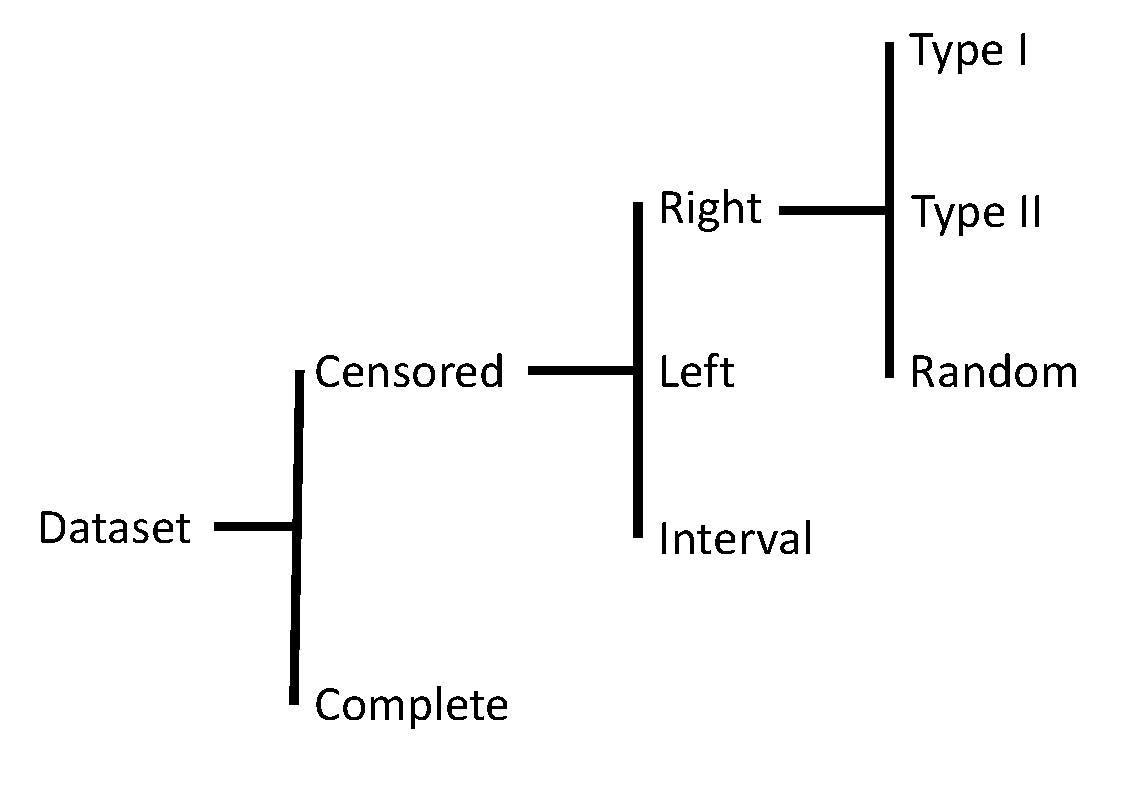
\includegraphics[width=0.8\textwidth]{images/censoring-taxonomy} 

}

\caption{Taxonomy of types of censoring.}\label{fig:surv-taxonomy}
\end{figure}

In order to illustrate the various types of censoring, we consider variations on the above Carcinogen Exposure study. First, consider a study design in which a sample of \(n\) rats are exposed at the same time point. The rats are followed for a period of two weeks, at which point the study is ended. This design emphasizes a situation in which the duration of the study is the primary constraint. If all rats develop a tumor during this two-week period, then the data set is complete.

\begin{definition}[Complete Data]
Describes a data set for which the event is observed on all subjects.
\end{definition}

When the data is complete, survival analysis reduces to a standard estimation problem that could be addressed using previously described methods.

Suppose, however, that some rats remain tumor-free at the end of the studied (Figure \ref{fig:surv-censoring-type-1}). These rats are censored. Since all rats began the study at the same point in time, any observation censored is censored at the same time point. In this case, we only know that the time until the rat develops the tumor is at least two weeks.

\begin{figure}

{\centering 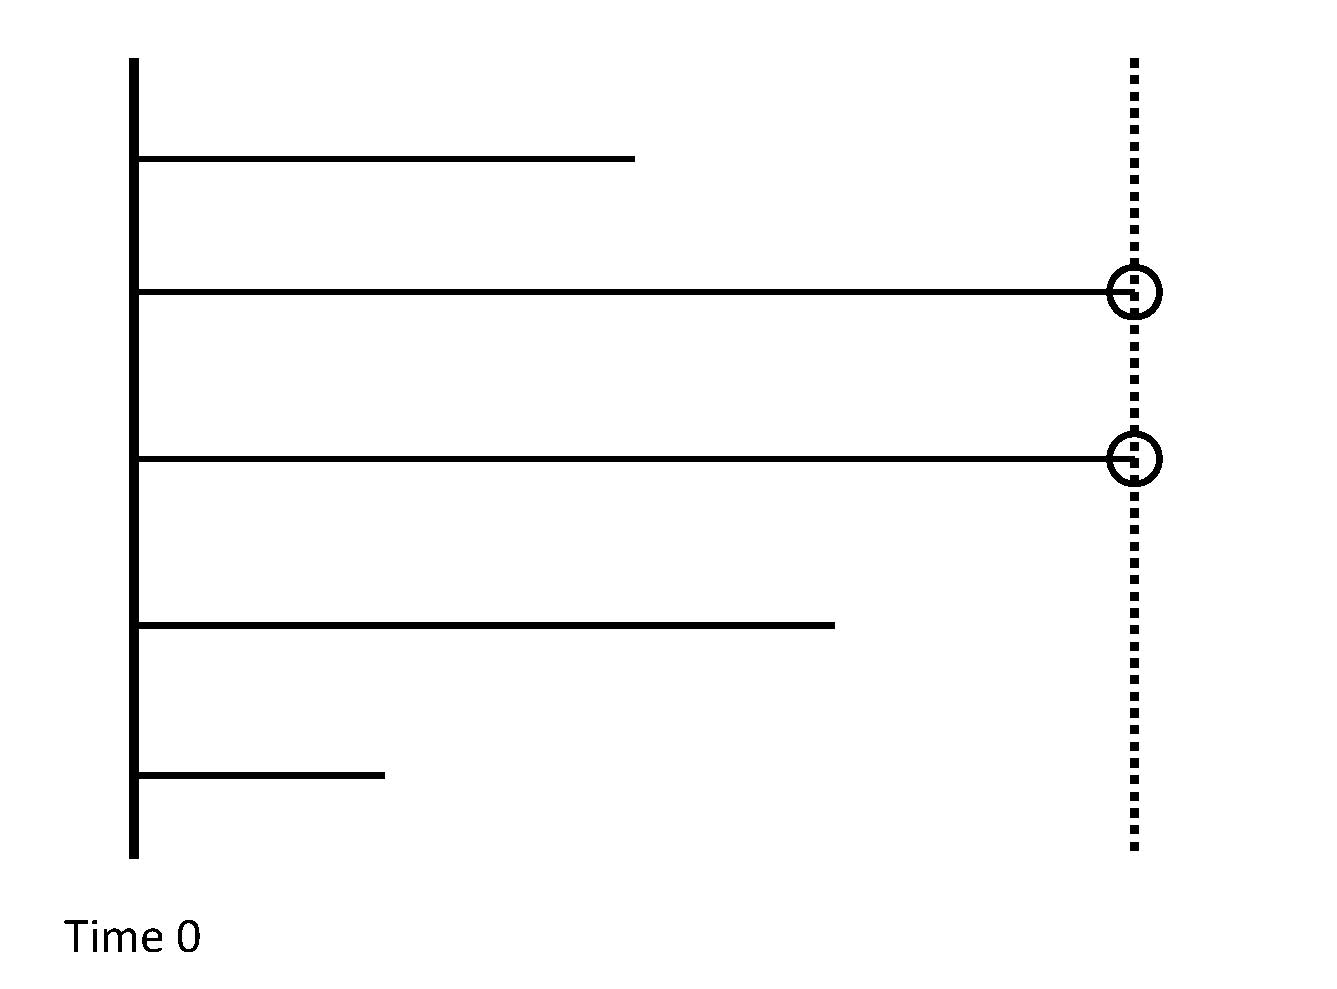
\includegraphics[width=0.8\textwidth]{images/censoring-type-1} 

}

\caption{Illustration of Type-I, right censoring.}\label{fig:surv-censoring-type-1}
\end{figure}

\begin{definition}[Right Censoring]
When a \emph{lower} bound is known on the time to event.
\end{definition}

\begin{definition}[Type I Censoring]
A form of right-censoring when the only source of censoring is the end of the study, for which the duration was pre-determined. Therefore, the time at which subjects are censored is the pre-determined study duration.
\end{definition}

In this study, the number of rats that remain tumor-free is random, and out of the control of the researchers. We contrast that with a design which says that the sample of \(n\) rats are exposed at the same time and the study continues until the first \(r\) rats develop a tumor (where \(r\) is chosen ahead of time). In this case, the length of the study is random. This study design might be chosen when running the study itself is cheap once the subjects are obtained; it ensures an adequate number of events to power the study. All rats remaining tumor-free past the \(r\)-th rat will be censored (Figure \ref{fig:surv-censoring-type-2}).

\begin{figure}

{\centering 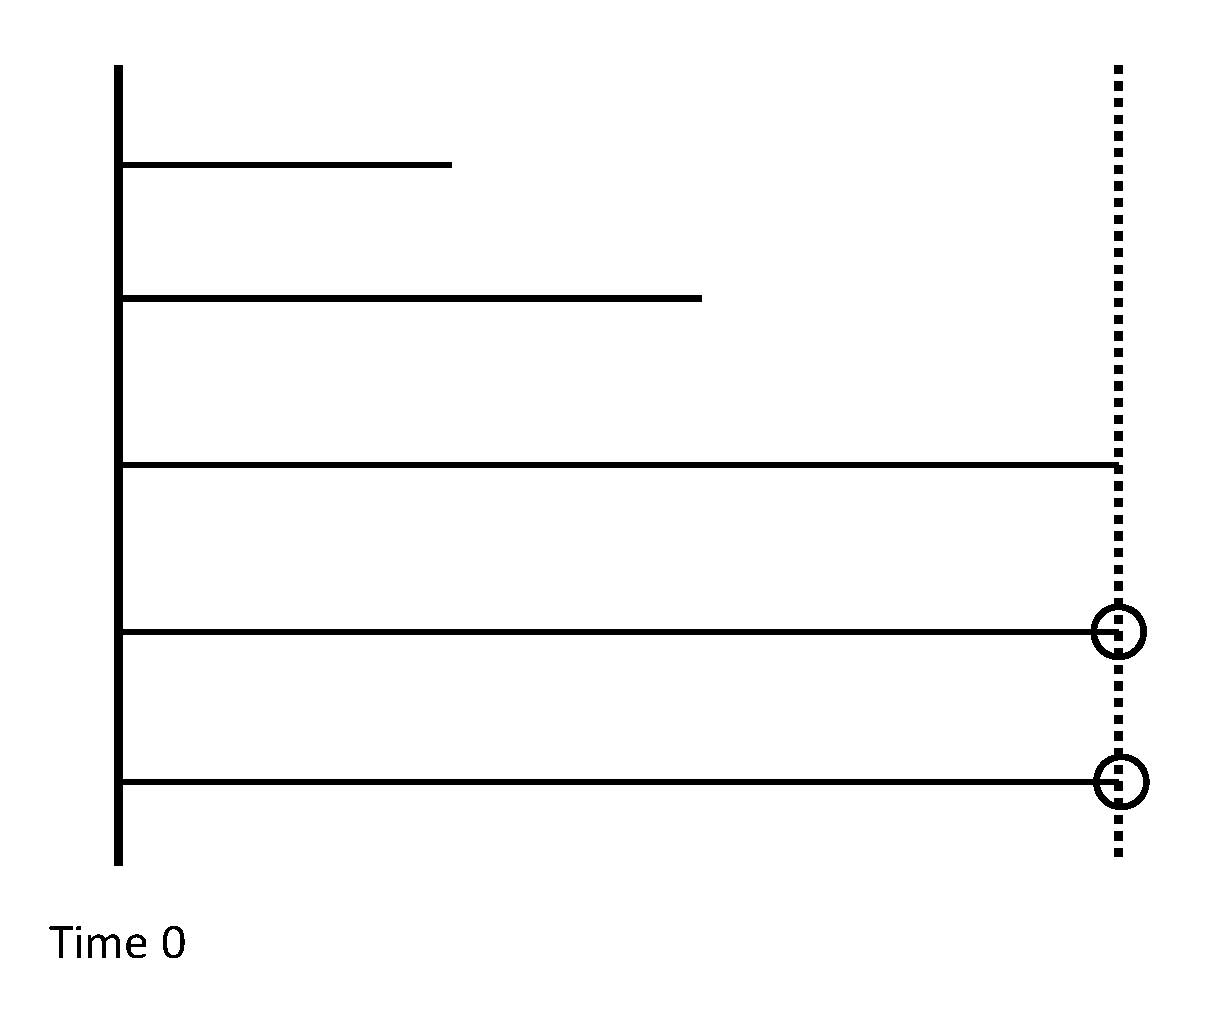
\includegraphics[width=0.8\textwidth]{images/censoring-type-2} 

}

\caption{Illustration of Type-II, right censoring.}\label{fig:surv-censoring-type-2}
\end{figure}

\begin{definition}[Type II Censoring]
A form of right-censoring when the only source of censoring is the end of the study, which is determined when the \(r\)-th event occurs and \(r\) is pre-determined. Therefore, the time at which subjects are censored is determined by the \(r\)-th event.
\end{definition}

Type I and Type II censoring tend to occur in controlled settings; in large-scale clinical trials involving human subjects, the source of censoring cannot be controlled. For example, suppose the particular breed of rat being studied is difficult to obtain. As a result, we are unable to obtain the \(n\) rats at the same time. Instead, each rat is obtained as it becomes available; the rat is then exposed to the carcinogen and followed for as long as possible (until it develops a tumor or the study ends). The study will end 2 months after obtaining the first rat. This results in staggered entry into the study, which as described above can be accounted for by thinking of ``time'' as ``time since exposure'' instead of ``time since study began.'' Many rats will experience the event. Others will not experience the event at the time the study ends. However, the length of time between entering the study and the study ending differs across those rats which are censored. Further, it is possible some rats are censored prior to the end of the study because they experience organ failure prior and die prior to the development of a tumor. The key observation is that the censoring times may differ for each rat (see Figure \ref{fig:surv-censoring-random}).

\begin{figure}

{\centering 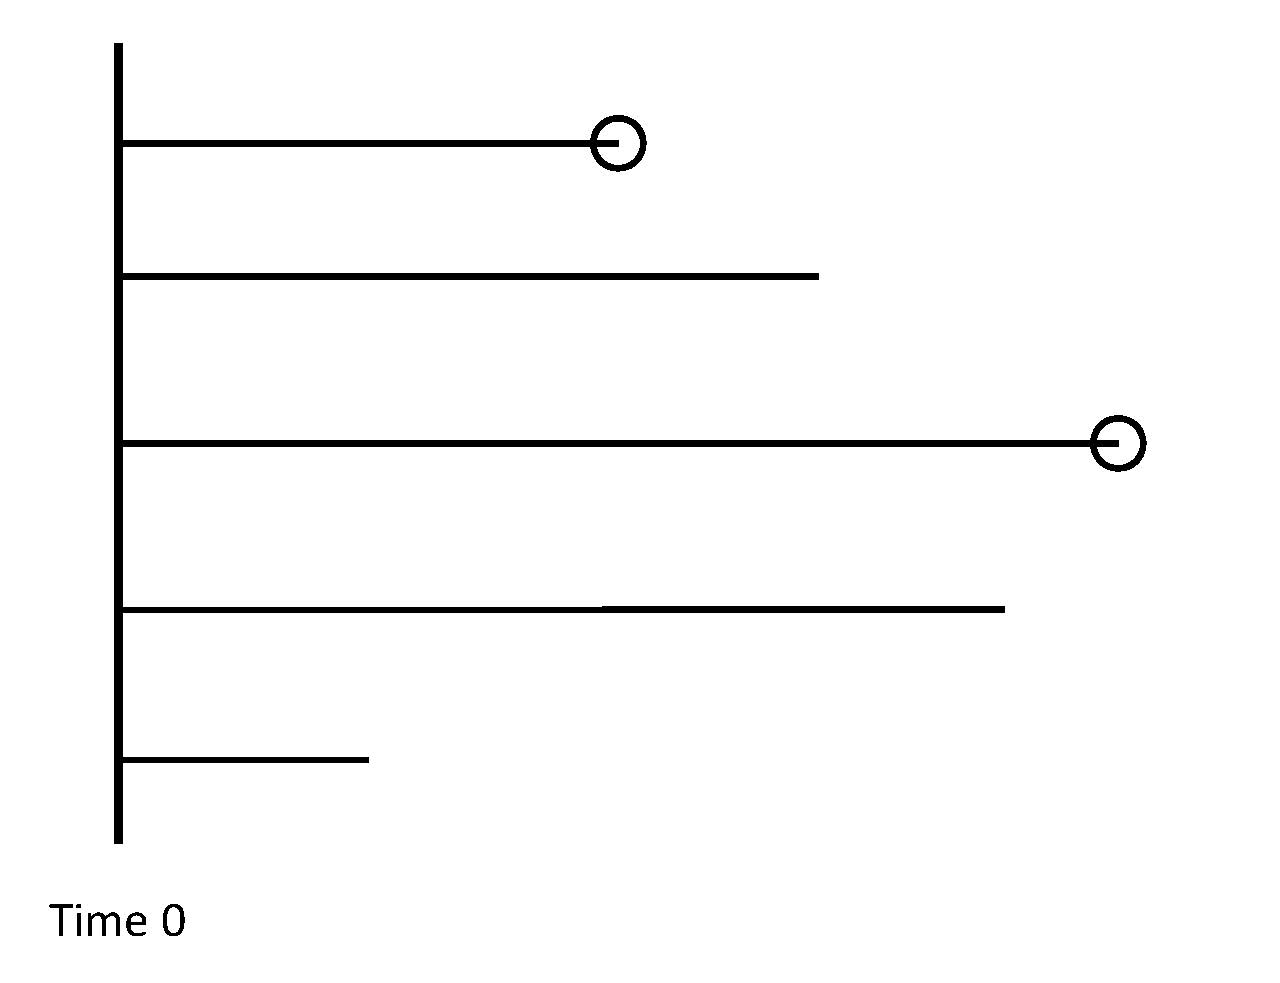
\includegraphics[width=0.8\textwidth]{images/censoring-random} 

}

\caption{Illustration of random right censoring, adjusted to patient time instead of study time.}\label{fig:surv-censoring-random}
\end{figure}

\begin{definition}[Random Censoring]
A form of right censoring when subjects are withdrawn from the study at any time. It is typically assumed that the event time and the censoring time are independent of one another.
\end{definition}

The assumption of independence between the censoring and event times is important. If only the healthiest patients are censored, then it is difficult to estimate the survival probability correctly; we assume that the reason each patient is censored has nothing to do with their underlying survival. This is fundamentally different than Type I or Type II censoring in which the healthiest subjects are those which are censored. By far, the most common type of censoring is random right censoring.

In each of the above cases, a lower bound was known on the event time, but there are other possibilities. Suppose the sample of \(n\) rats were exposed to the carcinogen at the same moment; however, this occurred at an off-site location. The rats are then transported to the lab, which takes several days. Upon arrival, it is discovered that \(m\) rats have already developed a tumor. For these rats, an upper bound is known on the event time.

\begin{definition}[Left Censoring]
When an \emph{upper} bound is known on the time to event.
\end{definition}

Finally, we consider the case in which the \(n\) rats are exposed to a carcinogen; the rats are assessed once weekly to determine if a tumor has developed. At the end of each week, the number who have developed a tumor is noted (Figure \ref{fig:surv-interval-censoring}). As a result, we do not know the exact day on which the tumor developed; we only know it occurred sometime within the last week. This creates both an upper and lower bound on the event time.

\begin{figure}

{\centering 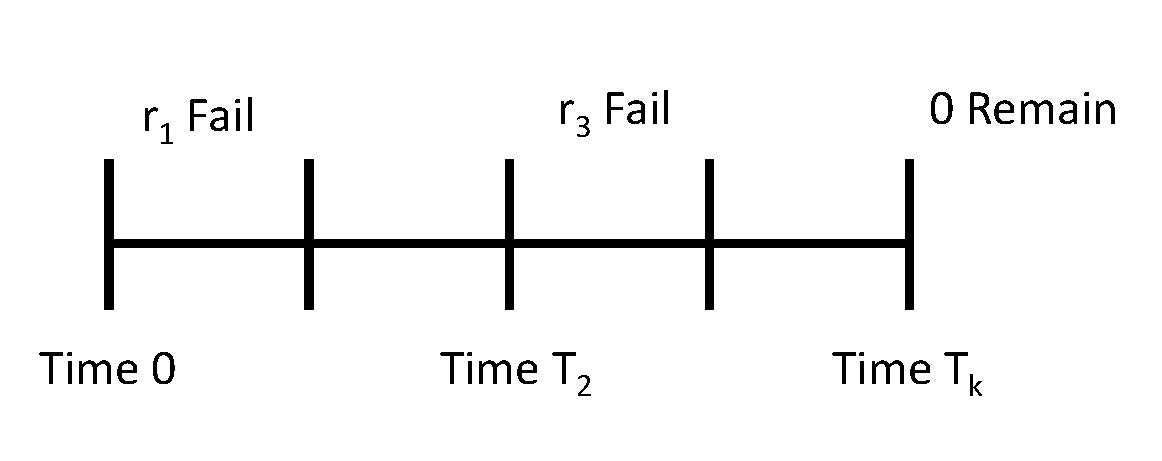
\includegraphics[width=0.8\textwidth]{images/censoring-interval} 

}

\caption{Illustration of interval censoring.}\label{fig:surv-interval-censoring}
\end{figure}

\begin{definition}[Interval Censoring]
When the event time is known to have occurred within some interval, but the exact time is unknown.
\end{definition}

Interval censoring results when only periodic assessment can be performed. Of course, it is impossible to measure an event time with infinite precision; therefore, it would seem all events are interval censored. In practice, we consider interval censoring to occur when the interval is larger than the smallest unit of time we would like to consider. For example, suppose for the Carcinogen Exposure example, we are interested in the number of days until the rat develops a tumor. In that case, daily assessments on the rats, while periodic, would not result in interval censoring; however, weekly assessments would be. In contrast, if we were interested in the number of hours until the rat develops a tumor, daily assessments would result in interval censoring.

Regardless of the type of censoring, it cannot be ignored. Due to censoring, we do not observe the survival time on all subjects, and this impacts the likelihood (Definition \ref{def:defn-likelihood}). Consider the case of right censoring; in that case, we observe the smaller of the survival time and the censoring time on each subject. We also are able to note whether our observation was the survival time or the censoring time.

\begin{definition}[Event Time and Censoring Indicator]
Let \(T_i\) and \(C_i\) represent the survival time and the censoring time for the \(i\)-th subject. When data is subject to right censoring, we observe

\[X_i = \min\left\{T_i, C_i\right\}\]

which is known as the \emph{event} time. We also note whether this observation was triggered by the actual event or censoring:

\[\delta_i = \begin{cases} 1 & \text{if } T_i \leq C_i \\ 0 & \text{if } T_i > C_i \end{cases}.\]

This is known as the \emph{censoring indicator}.
\end{definition}

\begin{rmdwarning}
Note that counter-intuitively, the ``censoring indicator'' actually indicates when the survival time is observed, not when an event is censored.
\end{rmdwarning}

Any analysis of survival data must account for the survival times and the censoring times; however, neither is directly observed on all subjects. As a result, standard methods are not applicable.

\hypertarget{surv-basic}{%
\chapter{Basic Estimation and Inference}\label{surv-basic}}

There are some studies in which we are interested in characterizing the overall survival; other studies seek to compare the survival across a small number of groups. In these situations, when the relation between survival and multiple characteristics of the subject are \emph{not} of primary interest, modeling is not necessary. In addition, having a grasp of these methods can help us better understand the benefits of modeling that we discuss in the next chapter.

As we have discussed in other settings, there are essentially three approaches to estimation: parametric, semiparametric, and nonparametric. This is true with time-to-event data as well. If we are willing to posit a model for the distribution of the survival times and the censoring times, we could potentially use likelihood methods to estimate the unknown parameters. While more popular among engineering disciplines, the biological sciences prefer semiparametric and nonparametic approaches. The methods discussed in this chapter are nonparametric in nature, while the model discussed in the next chapter is semiparametric.

\hypertarget{life-table-methods}{%
\section{Life-Table Methods}\label{life-table-methods}}

In some cohort studies, in which a large group is followed over the course of time with periodic ``check-ins,'' the exact event times are known to fall with key intervals. The origins of survival analysis are steeped in such studies. In such cases, life-table methods are used to characterize survival.

\begin{definition}[Life Table]
A method of estimating overall survival over key intervals of time, generally constructed for a single population.
\end{definition}

In order to illustrate the considerations in life-table methods, consider the following example.

\begin{example}[Hypertension]
A study was conducted to examine the efficacy of a new anti-hypertensive medication. A cohort of 146 patients with previous history of heart disease were treated and then followed over the next 10 years. The primary event of interest was death. A summary of the data is provided in Table \ref{tab:surv-hypertension-data}.
\end{example}

\begin{table}

\caption{\label{tab:surv-hypertension-data}Summary of Hypertension study investigating a new medication.}
\centering
\begin{tabular}[t]{lrrr}
\toprule
Years from Baseline & Number at Risk & Number of Deaths & Number Censored\\
\midrule
1 & 146 & 27 & 3\\
2 & 116 & 18 & 10\\
3 & 88 & 21 & 10\\
4 & 57 & 9 & 3\\
5 & 45 & 1 & 3\\
\addlinespace
6 & 41 & 2 & 11\\
7 & 28 & 3 & 5\\
8 & 20 & 1 & 8\\
9 & 11 & 2 & 1\\
10 & 8 & 2 & 6\\
\bottomrule
\end{tabular}
\end{table}

Let's consider how we should estimate the survival at time \(t = 5\); that is, what proportion of individuals survive past 5 years in the study? Notice that we observe 76 deaths during the first 5 years of follow-up; therefore, an initial guess might be

\[S(5) = 1 - \frac{\text{76 deaths over 5 years}}{\text{146 individuals}} = 0.479.\]

However, this assumes that every subject censored during the study lived the full five years. Remember, we do not know why the 3 subjects who were censored during the first year were lost to follow-up. All we know is that they were alive at the beginning of the study; we do not know if they died during the first year or survived through the end of the study. Assuming that the 29 censored individuals all survived through 5 years is quite optimistic, meaning that our estimate of survival is biased on the high-sided.

In order to correct this optimistic perspective, we might think to remove the censored subjects:

\[S(5) = 1 - \frac{\text{76 deaths over 5 years}}{\text{146 individuals} - \text{29 withdrawn}} = 0.350.\]

However, this essentially assumed these individuals never existed; however, we know that 3 of the subjects, for example, survived at least through the first 4 years. Excluding this information results in a pessimistic estimate, meaning our estimate of survival is biased on the low-side.

While these two extremes were illustrated over a five-year span, the same concerns exist on any single interval. For example, assuming the 3 subjects censored during the first year all survived the first year is optimistic; assuming they never existed is pessimistic. Life-table computations balance these two extremes. Our critical assumption is that the censoring occurs uniformly over each interval.

Consider the \emph{mortality} rate within the first interval, assuming subjects censored are done so uniformly over that first year. We can think of it as saying half the subjects who were censored should be removed from the study as if they never existed in that interval, and the other half survived to the end of the interval:

\[\widehat{m}(1) = \frac{27}{146 - 1.5} = 0.187.\]

This is an estimate of the probability a patient in this cohort dies during the first year. The survival probability during this interval is the probability of \emph{not} dying during the first year:

\[\widehat{S}(1) = 1 - \widehat{m}(1) = 0.813.\]

We can apply this adjustment on each interval. That is, the mortality within an interval is computed by considering the number of deaths over that interval as a fraction of the number of people at risk who entered that interval and assuming those censored exited uniformly over the interval. To survive to the end of any interval, you must have survived all previous intervals. This is captured in the following life-table computations.

\begin{definition}[Life Table Computations]
Let \(d_t\) represent the number of subjects that experienced the event during the \(t\)-th interval. Let \(w_t\) represent the number of subjects censored during the \(t\)-th interval. And, let \(n_{t}\) represent the number of subjects at risk at the start of the \(t\)-th interval.

Assuming censoring occurs uniformly over the interval, the estimated \emph{mortality} for the \(t\)-th interval is defined as

\[\widehat{m}(t) = \frac{d_t}{n_t - \frac{w_t}{2}}.\]

The estimated survival at the end of the \(t\)-th interval is given by

\[\widehat{S}(t) = \prod_{k=1}^{t} \left[1 - \widehat{m}(k)\right]\]
\end{definition}

We emphasize that we are estimating survival; the true survival is unknown. Of course, \(\widehat{S}(0) = 1\) since we begin with living subjects. Computing the survival as a product of interval-specific mortalities can be derived through a series of conditional probability statements; however, it captures the idea that a subject must survive each interval in turn. By looking one interval at a time, we reduce the bias in our estimate of survival. Employing these computations results in an estimated 5-year survival of \(\widehat{S}(5) = 0.417.\)

Of course, a point estimate does not allow for us to make inference on the true survival. In order to perform inference, we need to model the sampling distribution of our estimate.

\begin{definition}[Sampling Distribution of Life-Table Estimates]
As the sample size increases, the sampling distribution of the life-table estimate of survival can be modeled as

\[\frac{\widehat{S}(t) - S(t)}{\widehat{\sigma}^2} \sim N(0, 1)\]

where

\[\widehat{\sigma} = \widehat{S}(t) \sqrt{\sum\limits_{i=1}^t \frac{d_t}{\left(n_{t} - w_t/2\right)\left(n_{t} - w_t/2 - d_t\right)}}\]

and the estimate \(\widehat{S}(0) = 1\) has no error.
\end{definition}

Given the sampling distribution, it is possible to construct confidence intervals. However, using the classical

\[\widehat{S}(t) \pm (1.96) \widehat{\sigma}\]

to compute a 95\% confidence interval can result in bounds that extend beyond 0 or 1. Since \(S(t)\) is a probability, such bounds are unreasonable. One approach is to simply truncate the confidence limits at 0 or 1.

We note that this sampling distribution (and the resulting confidence intervals) are developed point-wise. That is, this is different than a confidence band meant to encompass the entire curve. For those unfamiliar with statistical theory, it is sufficient to keep in mind that the bounds were generated for a specific point in time \(t\).

Life-table methods are somewhat limited in their use as they apply to a single cohort and the survival times are grouped within intervals. However, the ideas discussed here are foundational to their generalization, which we now discuss.

\hypertarget{kaplan-meier-estimation}{%
\section{Kaplan-Meier Estimation}\label{kaplan-meier-estimation}}

The life-table estimation approach helps to highlight the key considerations when working with time-to-event data. To remove bias, we must carefully consider how the censored data is addressed. While life-table methods are not always applicable, we can generalize the results by considering how we would apply life-table methods with smaller and smaller intervals of time. Intuitively, the smaller we can make the interval, the less bias our estimates will have. To that end, we shrink the interval under consideration until it includes a single event time; then, we apply the life-table approach. This is known as the Kaplan-Meier estimate.

\begin{definition}[Kaplan Meier Estimator]
Also known as the product-limit estimator, this is the limit of the life-table estimate as we allow the intervals to shrink to a single event time:

\[\widehat{S}(t) = \prod_{t_i \leq t} \left(1 - \frac{d_{t_i}}{n_{t_i}}\right)\]

where \(t_i\) is the \(i\)-th event time where the event of interest was observed.
\end{definition}

There are a couple of things to note about this definition. Keep in mind that shrinking an interval to have no width is relative to what we consider the unit of time; if we are measuring survival time in days, then an interval only large enough to include a single event time would capture a single day. If survival time is measured in weeks, the interval would shrink to capture a single week. In the Kaplan-Meier estimator, the product is taken over all observed event times prior to \(t\). We emphasize that this does \emph{not} include censoring times.

\begin{rmdwarning}
The product-limit estimator does not change when an individual is censored. It is only updated when an individual experiences the event of interest.
\end{rmdwarning}

How then is censoring accouted for? Each time an event does occur and we update the estimator, we are adjusting the number of subjects at risk at that event time. When determining how many subjects are at risk, we do not consider previously censored subjects. This is similar to how the life-table estimate subtracted out the number of risk within each interval. Except, since our ``interval'' is a single event time, we do not need to think about those subjects being uniformly distributed over the interval; they all share the same time.

Kaplan-Meier curves (survival curves estimated using this method) are step-functions, with a step being taken at each time an individual subject experiences the event. Figure \ref{fig:surv-km-curves} gives an illustration of what these curves look like. Notice that if the last subjects in the sample are censored (which occurred in Group A in Figure \ref{fig:surv-km-curves}), then the survival probability will not drop to 0. In large scale-studies, it is not uncommon for the study to end with several patients remaining, meaning the survival curves stay relatively high.

\begin{figure}

{\centering 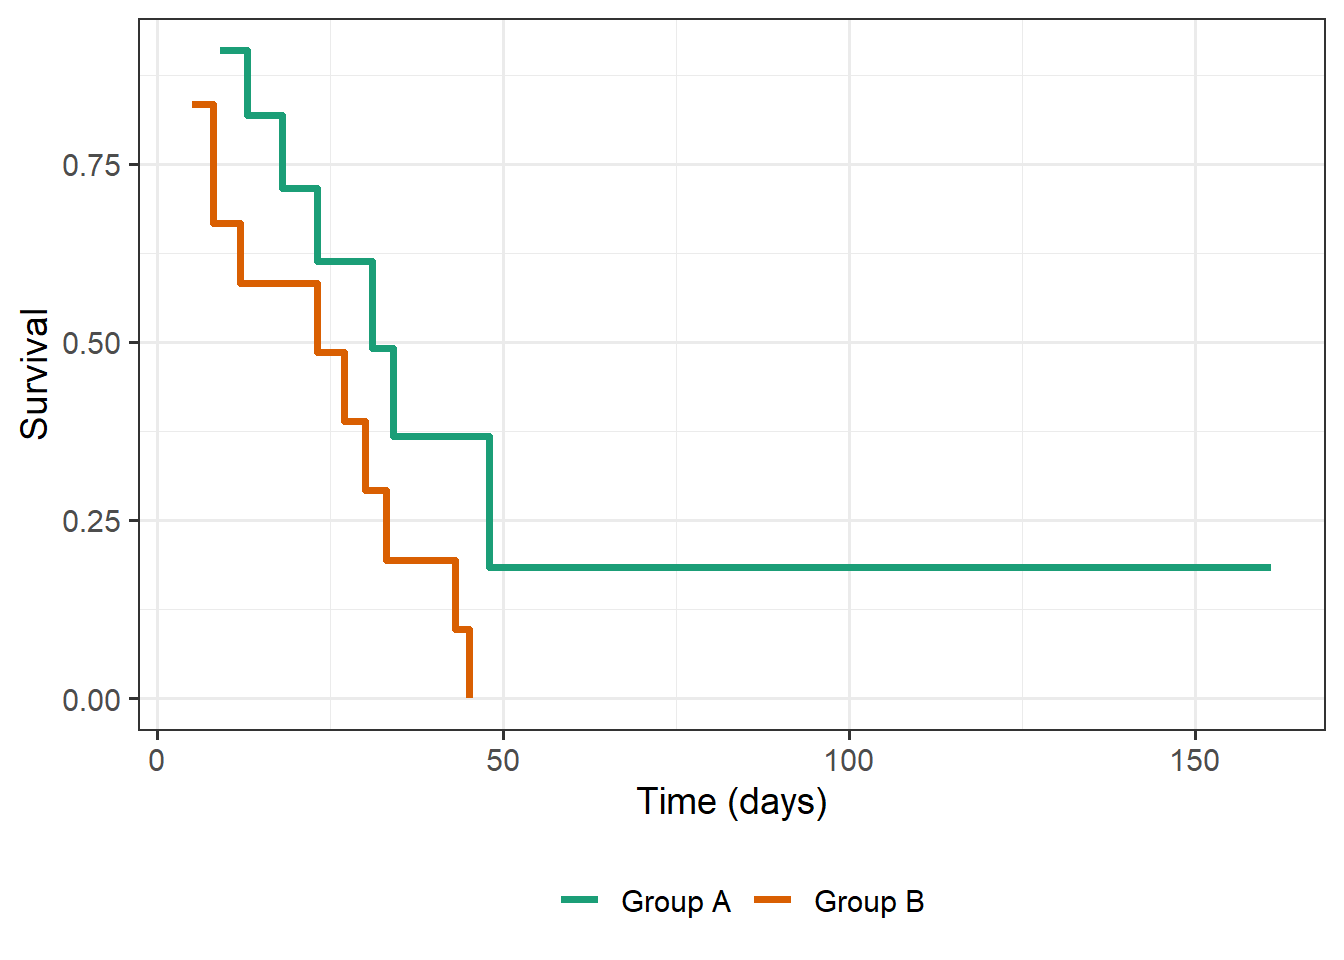
\includegraphics[width=0.8\textwidth]{./Images/surv-km-curves-1} 

}

\caption{Illustration of Kaplan-Meier estimates of survival for two groups.}\label{fig:surv-km-curves}
\end{figure}

Of course, a point estimate does not allow for us to make inference on the true survival. In order to perform inference, we need to model the sampling distribution of our estimate.

\begin{definition}[Sampling Distribution of Kaplan-Meier Estimates]
As the sample size increases, the sampling distribution of the life-table estimate of survival can be modeled as

\[\frac{\widehat{S}(t) - S(t)}{\widehat{\sigma}^2} \sim N(0, 1)\]

where

\[\widehat{\sigma} = \widehat{S}(t) \sqrt{\sum\limits_{t_i \leq t} \frac{d_{t_i}}{n_{t_i} \left(n_{t_i} - d_{t_i}\right)}}\]

and the estimate \(\widehat{S}(0) = 1\) has no error.
\end{definition}

As with life-table estimates, creating a classical confidence interval using the above standard error can result in confidence limits below 0 or above 1. It is common to construct the confidence interval on the hazard scale and then make a transformation back to the survival scale, which ensures confidence limits that are reasonable. This is the default approach in many statistical software packages.

\hypertarget{log-rank-test}{%
\section{Log-Rank Test}\label{log-rank-test}}

Estimating a survival curve is useful for describing the survival experience of a population; however, we are often interested in formally comparing the survival of two populations. One method of comparing two or more groups is the log-rank test.

\begin{definition}[Log-Rank Test]
Allows for formal comparison of \(k\) survival curves by testing the hypotheses

\[
\begin{aligned}
  H_0&: S_1(t) = S_2(t) = \dotsb = S_k(t) \ \forall t \quad \text{vs.} \\
  H_1&: \text{At least one } S_k \text{ differs for at least one } t
\end{aligned}
\]
\end{definition}

Notice that the above test is looking for \emph{any} differences whatsoever in the curves; that is, this is not a point-wise comparison but a comparison of the entire curves. The log-rank test compares the expected number of events at a given time with the observed number of events. Tests of this form are often referred to as Chi-Squared tests as the test statistic generally has a Chi-Square distribution in large sample sizes.

While the mathematical details for implementing the log-rank test are beyond the scope of the test, we note that the asymptotic distribution depends on the number of events observed, not the sample size. That is, power calculations are based on the number of events expected.

While the log-rank test allows for comparisons across groups, it does not allow us to quantify the effect of a predictor on the survival. In order to characterize the impact of a predictor on survival or to account for multiple predictors, we need a modeling approach for survival analysis.

\hypertarget{surv-cph}{%
\chapter{Cox Proportional Hazards Model}\label{surv-cph}}

Regression models allow us to quantify the effect of a set of predictors on the distribution of the response. While there are various regression methods for survival analysis, perhaps the most common is the Cox Proportional Hazards model, which we discuss in this chapter.

As the name of this chapter hints at, our modeling approach depends on the assumption of proportional hazards.

\begin{definition}[Proportional Hazards]
Let \(\lambda_1(t)\) and \(\lambda_2(t)\) represent the hazard functions for two different groups. The assumption of proportional hazards states that

\[\frac{\lambda_2(t)}{\lambda_1(t)} = e^{\gamma}\]

for some fixed \(\gamma\).
\end{definition}

Note that \(e^{\gamma}\) does not depend on time \(t\); that is, proportional hazards states that the ratio of two hazard functions, known as the hazard ratio, is constant over time. The reason for choosing to exponentiate the constant is because the hazard ratio must always be positive (since each hazard is positive for all values of \(t\)). This allows \(\gamma\), the natural logarithm of the hazard ratio, to play a role similar to the log-odds ratio (from logistic regression in Chapter \ref{nlm-logistic}). When \(\gamma = 0\), the hazard ratio is 1 and the two hazard functions are equal across all time (meaning the corresponding survival curves are equal across all time). When \(\gamma > 0\), the hazard ratio is larger than 1 and group 2 is more likely to experience the event (survival curve sits below) compared with group 1. When \(\gamma < 0\), the hazard ratio is below 1 and group 2 is less likely to experience the event (survival curve sits above) compared with group 1.

\begin{rmdwarning}
Proportional hazards is an assumption. It is not guaranteed to hold in any setting; however, it is a useful simplifying assumption and often does hold at least reasonably well.
\end{rmdwarning}

Early in this unit, we alluded to the idea that some characterizations of the distribution are easier to model than others. When censoring is present, it turns out that modeling the hazard turns out to be easier than modeling the survival function directly. Therefore, we want our model to allow the hazard function to depend upon predictors.

\begin{rmdtip}
Remember, a key idea in regression modeling is characterizing the distribution of the response through its parameters. We have spent a great deal of time in the text characterizing the mean and variance of the response with our regression models. Here, instead of the mean survival time, we are modeling the hazard function.
\end{rmdtip}

\begin{rmdtip}
Note that unlike modeling the mean response in which our model specifies a single value (the mean response) for a given set of predictors, in survival analysis, we are modeling an entire function. That is, for a given set of predictors, we are specifying the hazard function, which is a function over time.
\end{rmdtip}

We could model the hazard function under parametric assumptions (assuming a particular distribution for the event times and censor times, for example). However, Cox developed a semiparametric model which dominates the literature in the biological sciences.

\begin{definition}[Cox Proportional Hazards Model]
A model for the hazard function which enforces the assumption of proportional hazards; it has the following form:

\[\lambda\left(t \mid (\text{Predictors})_i\right) = \lambda_0(t) e^{\sum\limits_{j=1}^{p} \beta_j (\text{Predictor } j)_i},\]

where the form of \(\lambda_0(t)\), known as the baseline hazard, is not specified.
\end{definition}

This model separates the hazard function into a function of time alone (the baseline hazard) and a function of the predictors alone (the exponent). Since the baseline hazard is not specified, this is a semiparametric model; if this form were specified, you would have a fully parametric model. The baseline hazard function represents the hazard function when all predictors take the value of 0. That is, instead of a single intercept, we have a type of ``intercept-function.''

As a result of the product of the baseline hazard with the exponential, the predictors serve to scale the hazard function, making this a multiplicative model instead of additive. The name comes from the fact that the model enforces the assumption of proportional hazards. To see this, consider a simple model with only two predictors. Suppose one group of subjects has predictor values \(a\) and \(b\), respectively. Then, their hazard function has the form

\[\lambda_1(t \mid \text{Predictors}) = \lambda_0(t) e^{\beta_1 a + \beta_2 b}.\]

Let a second grou pof subjects have predictor values \(a + 1\) and \(b\), increasing the first predictor by 1 unit. Observe that their hazard function is

\[\lambda_2(t \mid \text{Predictors}) = \lambda_0(t) e^{\beta_1 (a + 1) + \beta_2 b}.\]

The baseline hazard function does not depend on the predictor values and so is shared between both groups. Consider the hazard ratio of group 2 compared with group 1:

\[
\begin{aligned}
  \text{HR} &= \frac{\lambda_2(t \mid \text{Predictors})}{\lambda_1(t \mid \text{Predictors})} \\
    &= \frac{\lambda_0(t) e^{\beta_1 a + \beta_1 + \beta_2 b}}{\lambda_0(t) e^{\beta_1 a + \beta_2 b}} \\
    &= e^{\beta_1}
\end{aligned}
\]

which does not depend on time \(t\) and therefore suggests the hazard functions are proportional across time. Further, it provides an interpretation for the parameters.

\begin{definition}
In a Cox Proportional Hazards (PH) model, the coefficient on the \(j\)-th predictor in the model is the log-hazard ratio associated with a one-unit increase in the \(j\) predictor, holding all other predictors fixed.
\end{definition}

Of course, we do not observe the actual values of the parameters; therefore, we estimate the parameters and therefore estimate the hazard function. This is done via a partial likelihood, the details of which are beyond the scope of this text; it was this partial likelihood which made the above model useful in practice. This allows us to estimate the parameters and even model their sampling distribution without needing to specify the baseline hazard function!

The simplicity of the Cox PH model has led to wide use. However, its apparent simplicity is also the source of many common mistakes when using the model in practice. We briefly note some of the more common errors researchers make:

\begin{itemize}
\tightlist
\item
  Using predictors that were gathered after baseline or the assignment of the treatment of interest. If we observe something after we ``start the clock,'' then its very observation implies the subject is event-free at this point in time.
\item
  Forgetting that proportional hazards assumption implies one curve is superior regardless of time. If you estimate the survival curves from a proportional hazards model, one treatment group will always be superior to the other (though the difference may be statistically insignificant). This is because the proportional hazards assumption states that one survival curve always sits above the other.
\item
  Neglecting that this framework can be generalized to handle repeated outcomes and time-dependent predictors. As stated above, we do not allow the predictors to depend on time, but this framework generalizes nicely to allow this (or multiple types of events). Some researchers perform unnecessary simplifications when the method should be generalized.
\end{itemize}

We have seen the appeal of semi-parametric models throughout the course. Given enough data, they often provide efficient estimation without requiring many conditions on the data generating process. While the Cox PH model does avoid specifying the form of the survival distribution, it does carry certain conditions:

\begin{itemize}
\tightlist
\item
  The portion of the model involving the predictors is correctly specified.
\item
  The predictors are linearly related to the log-hazard function.
\item
  The affect of changing a predictor in isolation results in proportional hazards; this is enforced by the model. It implies that survival curves should not cross for different groups.
\item
  The censoring time is independent of the survival time.
\end{itemize}

As with other forms of regression models, residual plots can be created to assess the first three conditions. The final condition must be assessed by discipline expertise. The complication is that there is not a single definition of a residual with time-to-event data. And, different types of residuals are useful for assessing different conditions. While beyond the scope of this text, we want to note that there are methods for relaxing many of these conditions while still remaining in the same general framework, making the Cox PH model extremely flexible.

\hypertarget{refs}{}
\begin{CSLReferences}{1}{0}
\leavevmode\vadjust pre{\hypertarget{ref-Rosner2006}{}}%
Rosner, Bernard. 2006. \emph{Fundamentals of Biostatistics}. 6th ed. CA: Thomson-Brooks/Cole.

\leavevmode\vadjust pre{\hypertarget{ref-Vittinghoff2012}{}}%
Vittinghoff, Eric, David V. Glidden, Stephen C. Shiboski, and Charles E. McCulloch. 2012. \emph{Regression Methods in Biostatistics: Linear Logistic, Survival, and Repeated Measures Models}. 2nd ed. NY: Springer-Verlag.

\leavevmode\vadjust pre{\hypertarget{ref-Wickham2014}{}}%
Wickham, Hadley. 2014. {``Tidy Data.''} \emph{Journal of Statistical Software} 59 (10): 1--23.

\end{CSLReferences}

\end{document}
